\subsection{Construcción}

En esta sección se describe la construcción de la propuesta del sistema, la cual se divide en dos partes fundamentales: la API y la interfaz
de usuario.

\subsubsection{API (Backend)}

\paragraph{Dependecias de la API}
Las dependencias utilizadas en la API se gestionaron mediante npm (Node Package Manager), el cual es un gestor de paquetes para el lenguaje
de programación JavaScript, el cual permite instalar, actualizar y eliminar paquetes mediante un archivo de configuración llamado package.json.
En en Anexo \ref{apendix:dependencias-api} muestra el archivo package.json con las dependencias utilizadas en la API.

\paragraph{Configurar variables de entorno de la API}
Para la configuración de las variables de entorno de la API se utilizó un archivo .env, el cual contiene las propiedades de la
aplicación, como la URL de conexión a la base de datos, la configuración para el envío de correos electrónicos, la configuración del servicio de
almacenamiento de imágenes, la configuración del servicio de notificaciones push y la configuración del servicio de Google Maps y el secret key
para la generación de tokens JWT. En el Anexo \ref{apendix:configuracion-env-api} se muestra el archivo .env con las variables de entorno de la API.

\paragraph{Configurción de la seguridad de la API}
Para la configuración de la seguridad de la API, se utilizó una estrategia de autenticación basada en JWT (Json Web Token) y el sistema
de Guards que proporciona NestJS. La estrategia de autenticación JWT se implementó mediante un middleware que verifica la validez del
token JWT en cada solicitud realizada a la API. Este middleware se encarga de extraer el token del encabezado de autorización y verificar
la firma del token con la clave secreta, además de comprobar si el usuario tiene los permisos necesarios para acceder a los recursos
protegidos. En el Anexo \ref{apendix:configuracion-seguridad-api} se muestra la configuración de la seguridad de la API.

\paragraph{Accesso y persistencia de datos}
Para administrar el acceso y la persistencia de datos en la API, se utilizó un ORM (Object-Relational Mapping) llamado PrismaJS, que
emplea un lenguaje de modelado de datos propio para definir las entidades de la aplicación mediante un archivo "schema.prisma", el cual
contiene los modelos y relaciones de la base de datos, como se muestra en el Anexo \ref{apendix:modelo-datos-api}. PrismaJS facilita
la interacción con la base de datos PostgreSQL mediante consultas SQL generadas automáticamente a partir de las operaciones CRUD (Create,
Read, Update, Delete) realizadas en la API, lo que permite mantener una sincronía entre TypeScript y la base de datos. De este modo,
cualquier cambio en el esquema de la base de datos se reflejará automáticamente en el código de la API.

\paragraph{Esquema de la base de datos}
Una vez definidos los modelos en el esquema de prisma se procedió a realizar la migración de la base de datos, para ello se utilizó el
comando "npx prisma migrate dev", el cual crea las tablas en la base de datos PostgreSQL a partir del esquema definido
en el archivo schema.prisma, como se muestra en la Figura \ref{fig:migracion-base-datos}.

\begin{landscape}
    \begin{figure}[H]
        \centering
        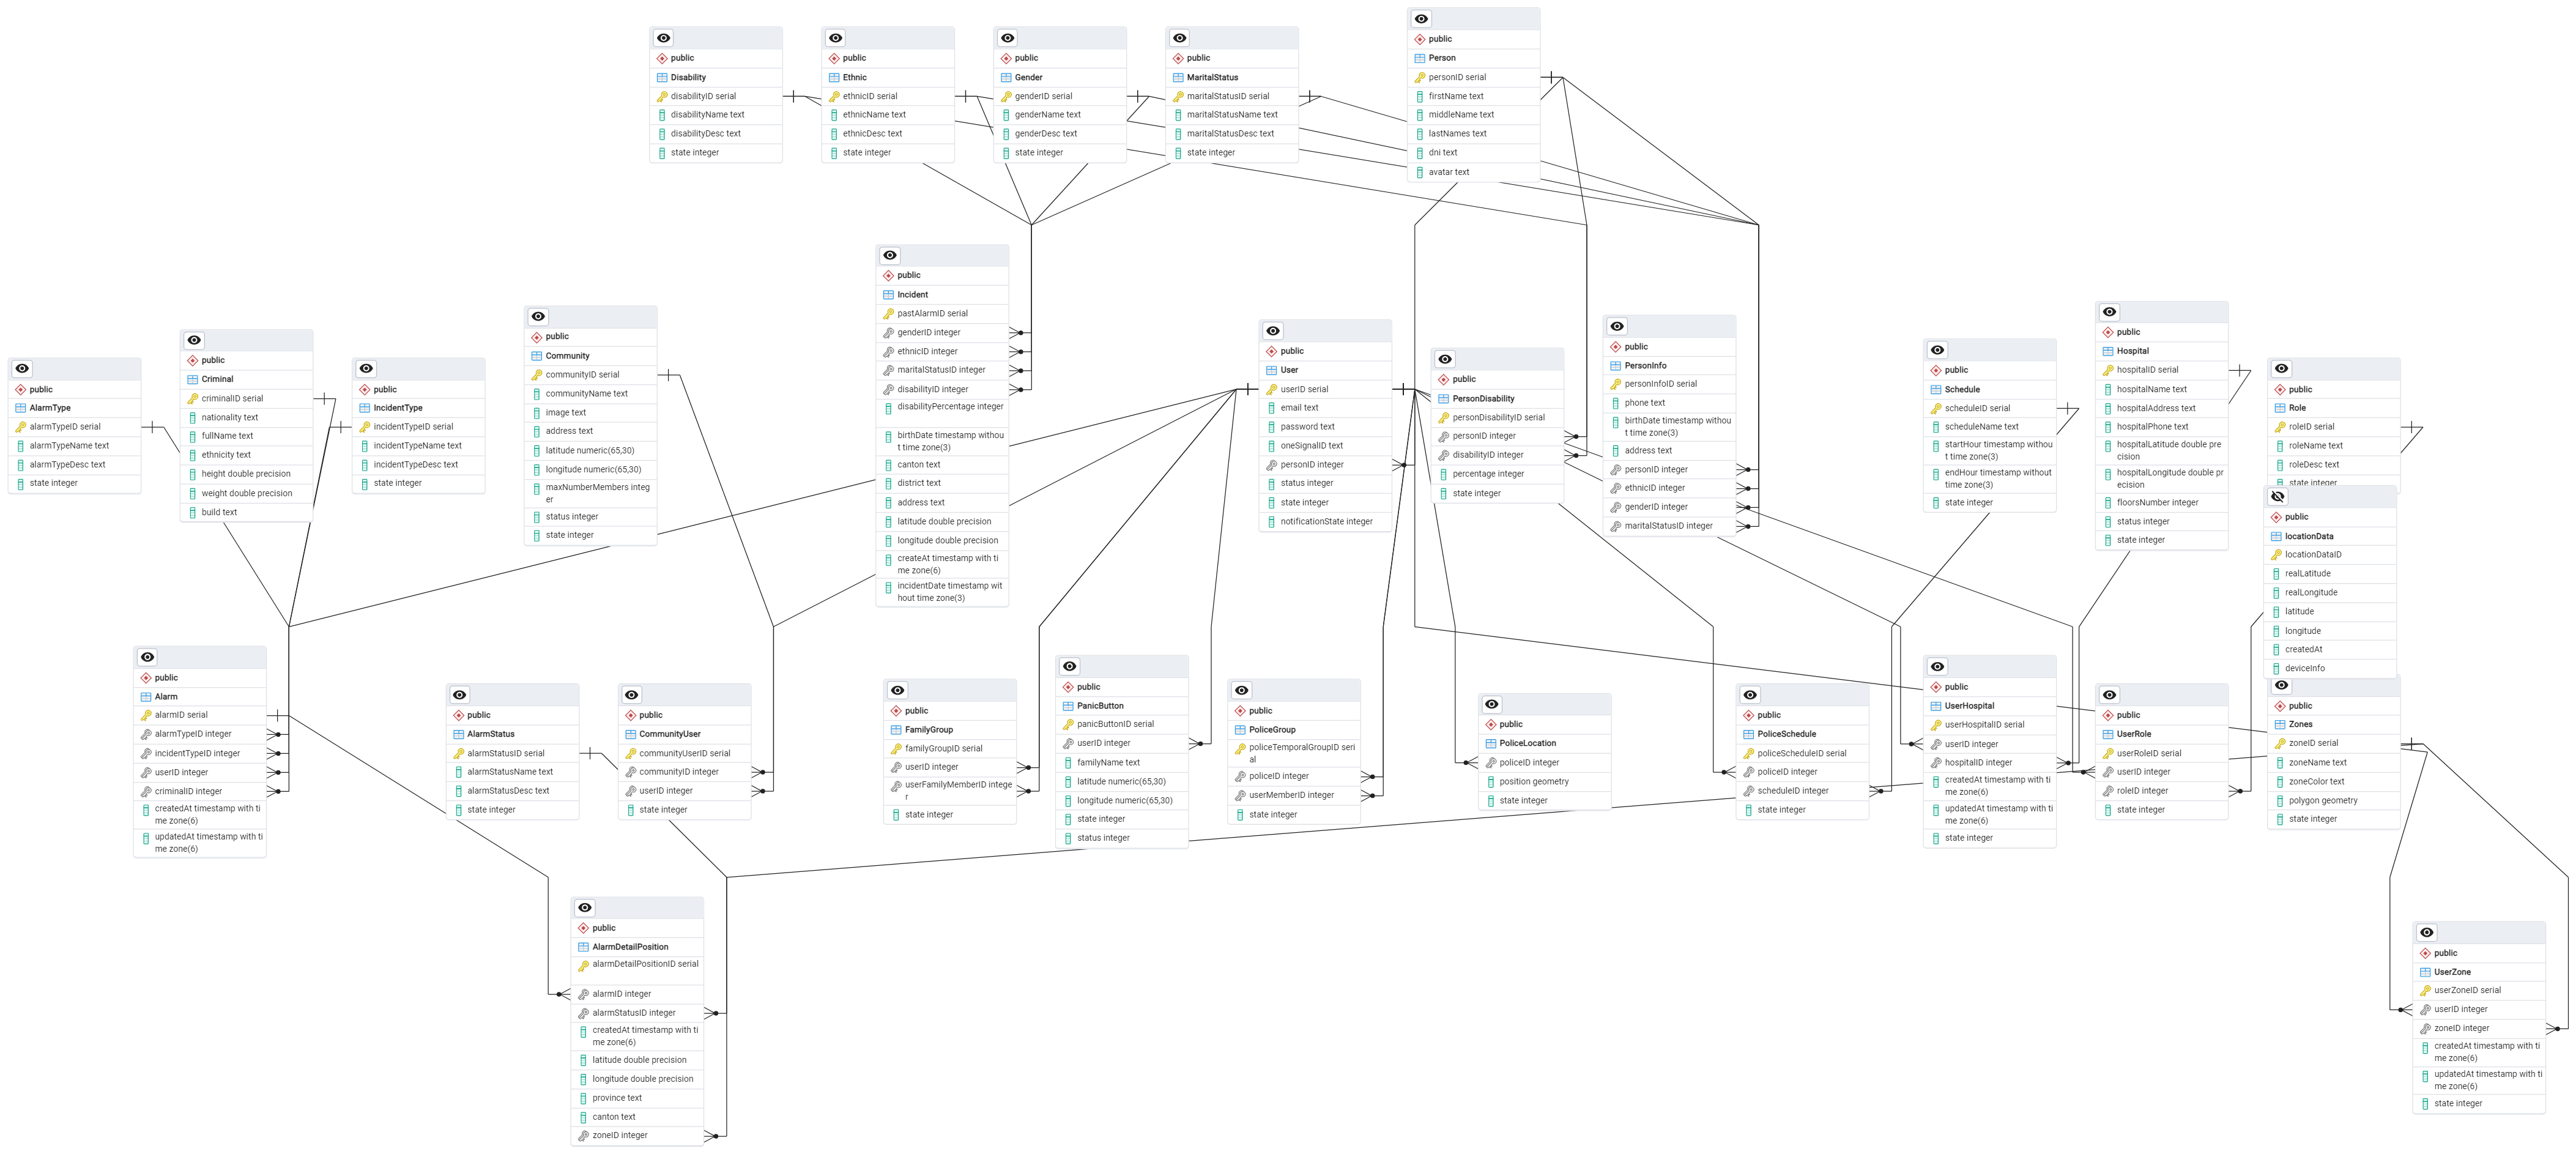
\includegraphics[width=1.7\textwidth]{chapters/III-resultados-y-discusion/resources/images/migracion-base-datos.png}
        \caption{Migración de la base de datos con PrismaJS.}
        \label{fig:migracion-base-datos}
    \end{figure}
\end{landscape}

\paragraph{Validación de datos}
Para la validación de datos en la API, se utilizó la librería class-validator, la cual permite definir reglas de validación mediante
decoradores en las clases de los modelos de datos. Estos decoradores se encargan de validar los datos de entrada en las solicitudes
realizadas a la API, como se muestra en el Anexo \ref{apendix:validacion-datos-api}.

\paragraph{Envío de correos electrónicos}
Para el envío de correos electrónicos en la API se utilizó la librería de nest mailer, la cual trabaja sobre la librería nodemailer
para el envío de correos electrónicos. Para la configuración del servicio de envío de correos se utilizó el SMTP (Simple Mail Transfer
Protocol) de Gmail, este permite enviar correos electrónicos utilizando la cuenta de Gmail del usuario administrador, como se muestra
en el Anexo \ref{apendix:envio-correos-api}.
\bigbreak

Para plantilla de correo electrónico se utilizó el sistema de plantillas de handlebars, el cual permite generar HTML dinámico a partir
de un archivo de plantilla y datos de contexto en formato JSON. En el Anexo \ref{apendix:plantilla-correo-api} se muestra la plantilla
de correo electrónico utilizada para recuperar la contraseña de un usuario.

\paragraph{Configuración y uso del servicio de almacenamiento de imágenes}
Para el almacenamiento de imágenes en la API se utilizó el servicio de Cloudinary, el cual permite almacenar y gestionar imágenes en la nube.
Cloudinary provee una librería para NodeJS que facilita la subida de imágenes, para la configuración se requiere obtener una api key, api secret
y cloud name, como se muestra en el Anexo \ref{apendix:configuracion-cloudinary-api}.
\bigbreak

Una vez configurado el servicio de Cloudinary, se procedió a implementar la subida de imágenes en la API. Para ello, se creó un servicio
que abstrae la lógica de la librería de Cloudinary y permite subir imágenes a Cloudinary y obtener la URL de la imagen subida, como se
muestra en el Anexo \ref{apendix:subida-imagenes-api}. Este servicio se inyectó en el controlador de la API y se utilizó en el endpoint
de creación de usuarios para subir la fotografía de perfil del usuario, como se muestra en el Anexo \ref{apendix:subida-imagenes-usuario-api}.

\paragraph{Configuración y uso del servicio de notificaciones push}
Para el envío de notificaciones push en la API, se utilizó el servicio de OneSignal, que permite enviar notificaciones a dispositivos
móviles y navegadores web. OneSignal provee una librería para Node.js que facilita el envío de notificaciones push. Para la configuración,
se requiere obtener una app ID y una API key, como se muestra en el Anexo \ref{apendix:configuracion-onesignal-api}.
\bigbreak

Con la configuración realizada, se procedió a implementar una abstracción del API de la librería de OneSignal en un servicio que proporciona
una instancia del cliente para el envío de notificaciones, como se puede visualizar en el Anexo \ref{apendix:configuracion-onesignal-api}. Este servicio
se inyectó en el controlador del módulo de notificaciones push, en el cual se implementó un endpoint para enviar notificaciones a los miembros
del grupo familiar del usuario y a los policías dentro de la zona de emergencia, como se puede observar en el Anexo \ref{apendix:envio-notificaciones-api}.

\paragraph{Modulos}
NestJS permite organizar la aplicación en módulos, los cuales contienen controladores, servicios y dto (Data Transfer Object). Los módulos se encargan
de importar y exportar los componentes de la aplicación, lo que facilita la reutilización de código y la separación de responsabilidades. En el Anexo
\ref{apendix:modulos-api} se muestra la estructura de los módulos de la API.

\paragraph{Controladores}
Los controladores en NestJS son clases que se encargan de gestionar las solicitudes HTTP y devolver una respuesta al cliente. Cada controlador
contiene una serie de métodos que se corresponden con los diferentes endpoints de la API además de los decoradores que definen los permisos de
acceso a los recursos protegidos. En el Anexo \ref{apendix:controladores-api} se muestra la estructura de los controladores de la API.

\paragraph{Servicios}
Los servicios en NestJS son clases que contienen la lógica de negocio de la aplicación y se encargan de interactuar con la base de datos y otros
servicios externos. Los servicios se inyectan en los controladores y otros servicios mediante la inyección de dependencias, lo que permite reutilizar
la lógica de negocio en diferentes partes de la aplicación. En el Anexo \ref{apendix:servicios-api} se muestra la estructura de los servicios de la API.

\paragraph{DTO (Data Transfer Object)}
Los DTO en NestJS son clases que se utilizan para transferir datos entre los controladores y los servicios de la aplicación. Los DTO definen la
estructura de los datos que se envían y reciben en las solicitudes HTTP, lo que facilita la validación de datos y la prevención de errores en la
aplicación. En el Anexo \ref{apendix:dto-api} se muestra la estructura de los DTO de la API.

\paragraph{Documentación de la API}
Para la documentación de la API se utilizó la librería Swagger, la cual permite generar una documentación interactiva de la API a partir de los
decoradores y comentarios en el código fuente. La documentación de la API se puede visualizar en la ruta /api-docs, como se muestra en la Figura
\ref{fih:documentacion-api}.

\begin{figure}[H]
    \centering
    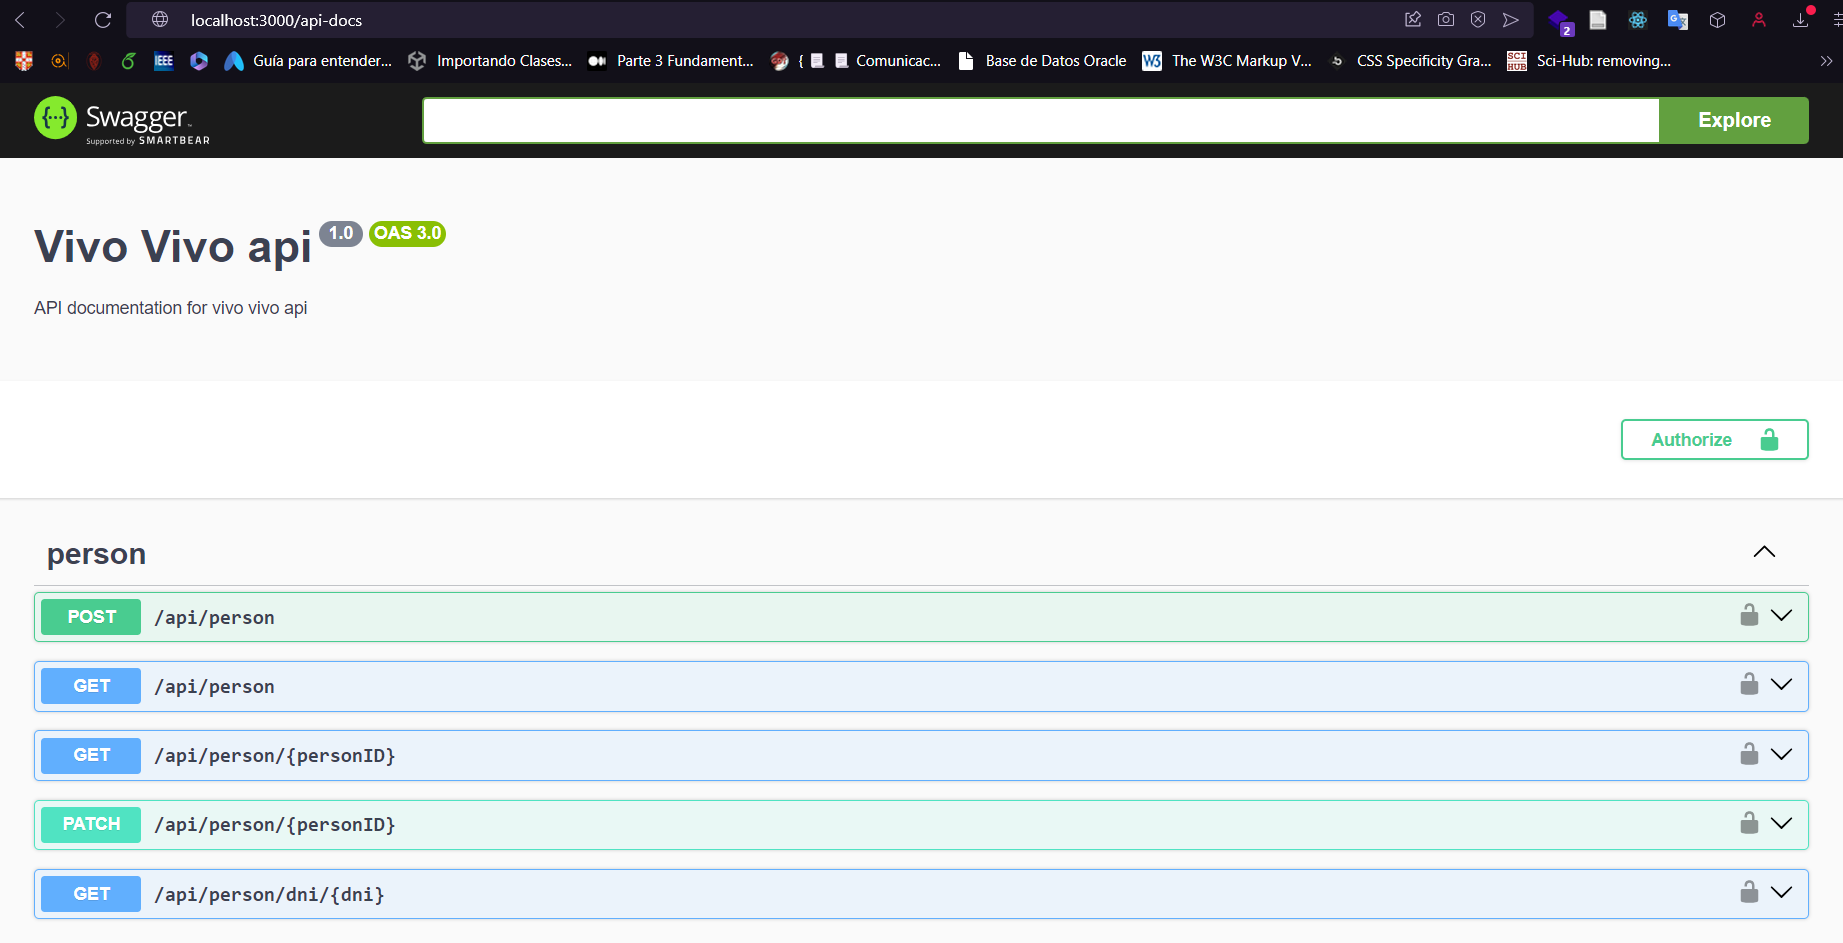
\includegraphics[width=0.8\textwidth]{chapters/III-resultados-y-discusion/resources/images/documentacion-api.png}
    \caption{Documentación de la API con Swagger.}
    \label{fih:documentacion-api}
\end{figure}

\subsubsection{Interfaz de usuario (Frontend)}

\textbf{Sistema web}
\bigbreak

\paragraph{Dependencias del sistema web}
Para crear el proyecto de NextJS se utilizó el comando "npx create-next-app@latest", el cual crea una aplicación de
NextJS con una estructura de carpetas y archivos predefinida. Las dependencias utilizadas en el sistema web se gestionaron mediante
npm y el archivo de configuración package.json. En el Anexo \ref{apendix:dependencias-web} se muestra dependencias utilizadas en el
sistema web.

\paragraph{Configuración de variables de entorno del sistema web}
Para la configuración de las variables de entorno del sistema web se utilizó un archivo .env.local, el cual contiene las propiedades
de la aplicación, como la URL de la API, el api key de Google Maps, la url y secret para la autenticación y la url
para obtener las imágenes de Cloudinary. En el Anexo \ref{apendix:configuracion-env-web} se muestra el archivo .env.local con las
variables de entorno del sistema web.

\paragraph{Configuración de la aplicación}
En Next.js, la configuración global de la aplicación se realiza mediante Providers y Contexts, los cuales permiten compartir datos y
funcionalidades entre los componentes. En el Anexo \ref{apendix:configuracion-aplicacion-web} se muestra la configuración para los
proveedores de sesión, componentes de UI, notificaciones y gestión de datos en el sistema web.

Las rutas de la aplicación en Next.js se crean mediante el gestor de archivos, el cual permite crear rutas dinámicas y estáticas
siguiendo una estructura "carpeta/page.ts", donde "carpeta" es el nombre de la ruta y "page.ts" es el archivo de la página. En el
Anexo \ref{apendix:rutas-aplicacion-web} se muestra la estructura de las rutas de la aplicación web.

\paragraph{Inicio de sesión}
El inicio de sesión en el sistema web se realiza mediante un formulario en el cual el usuario ingresa su correo electrónico y
contraseña, como se muestra en la Figura \ref{fig:inicio-sesion-web}. Estos campos son validados mediante la librería Zod, la
cual permite definir esquemas de validación para los datos de entrada en los formularios, como se puede observar en el Anexo
\ref{apendix:validacion-datos-web}. Una vez validados los datos, se envía una solicitud POST a la API para autenticar al usuario
y obtener un token JWT, el cual se almacena en la sesión del navegador para mantener la sesión activa, en el Anexo
\ref{apendix:guardar-token-web} se muestra el código para guardar el token en la sesión del navegador.

\begin{figure}[H]
    \centering
    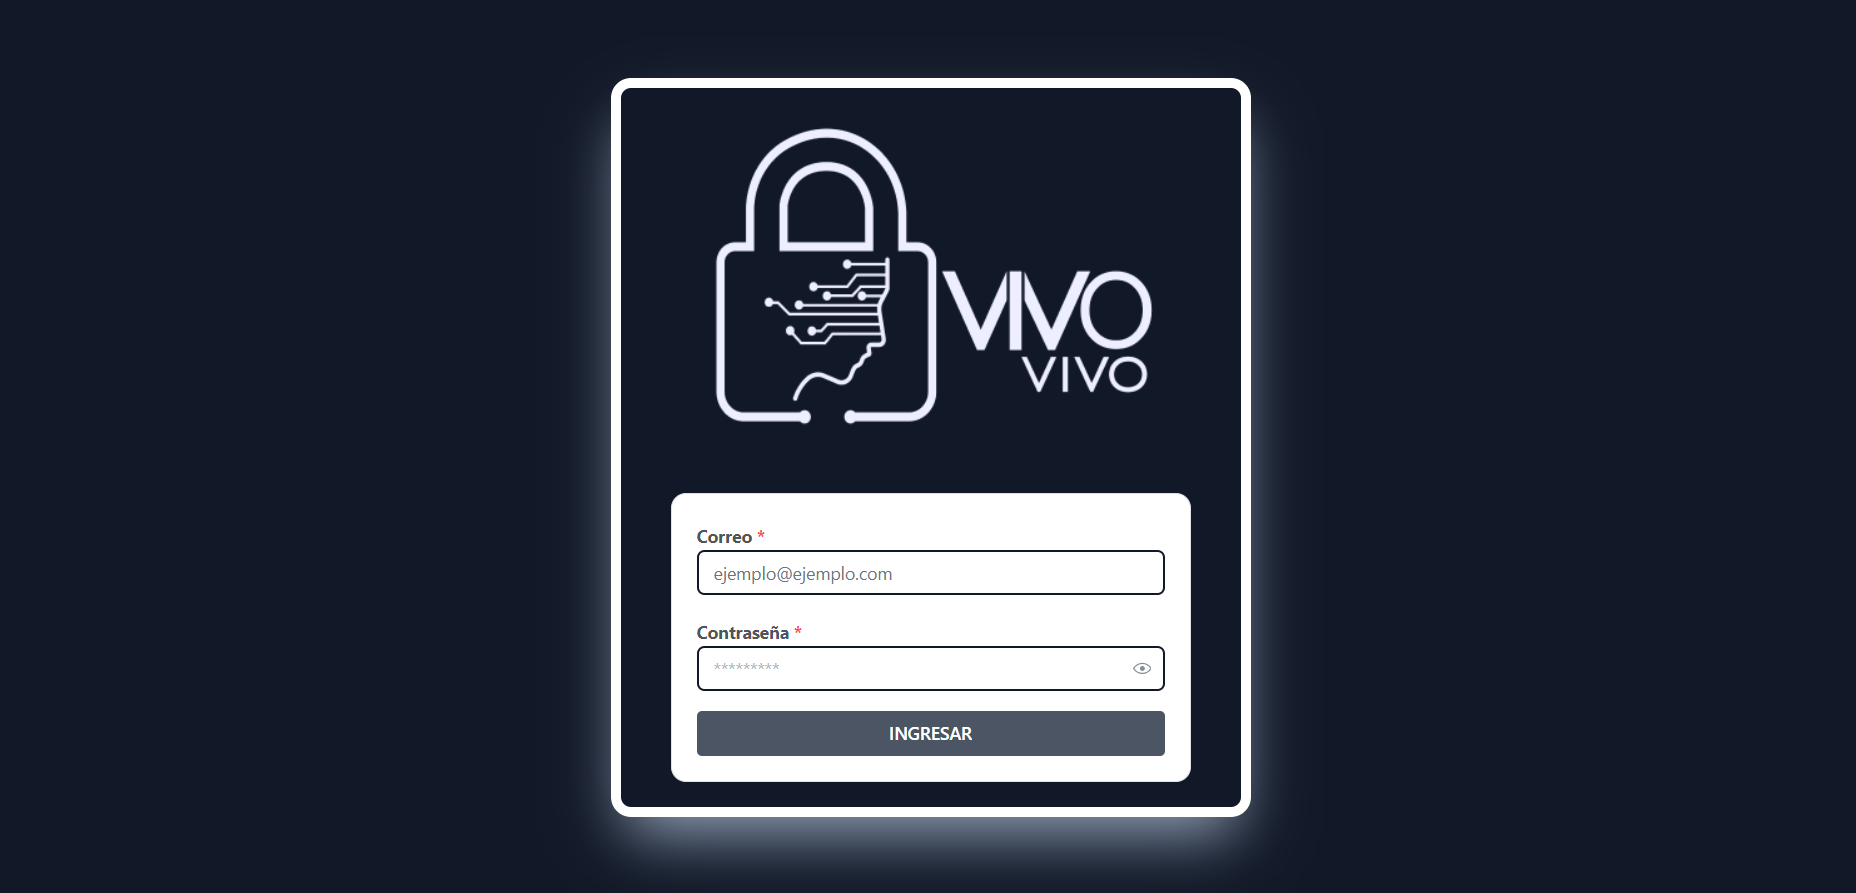
\includegraphics[width=0.8\textwidth]{chapters/III-resultados-y-discusion/resources/images/inicio-sesion-web.png}
    \caption{Inicio de sesión en el sistema web.}
    \label{fig:inicio-sesion-web}
\end{figure}

\paragraph{Menú de usuario}
El menú de usuario en el sistema web permite al usuario administrador acceder a las opciones de la aplicación al hacer clic en
el botón de configuración en la esquina superior derecha de la pantalla. Al hacer esto, se muestra un menú desplegable en el
cual se encuentran las opciones de cambiar contraseña y cerrar sesión, como se muestra en la Figura \ref{fig:menu-usuario-web}.

\begin{figure}[H]
    \centering
    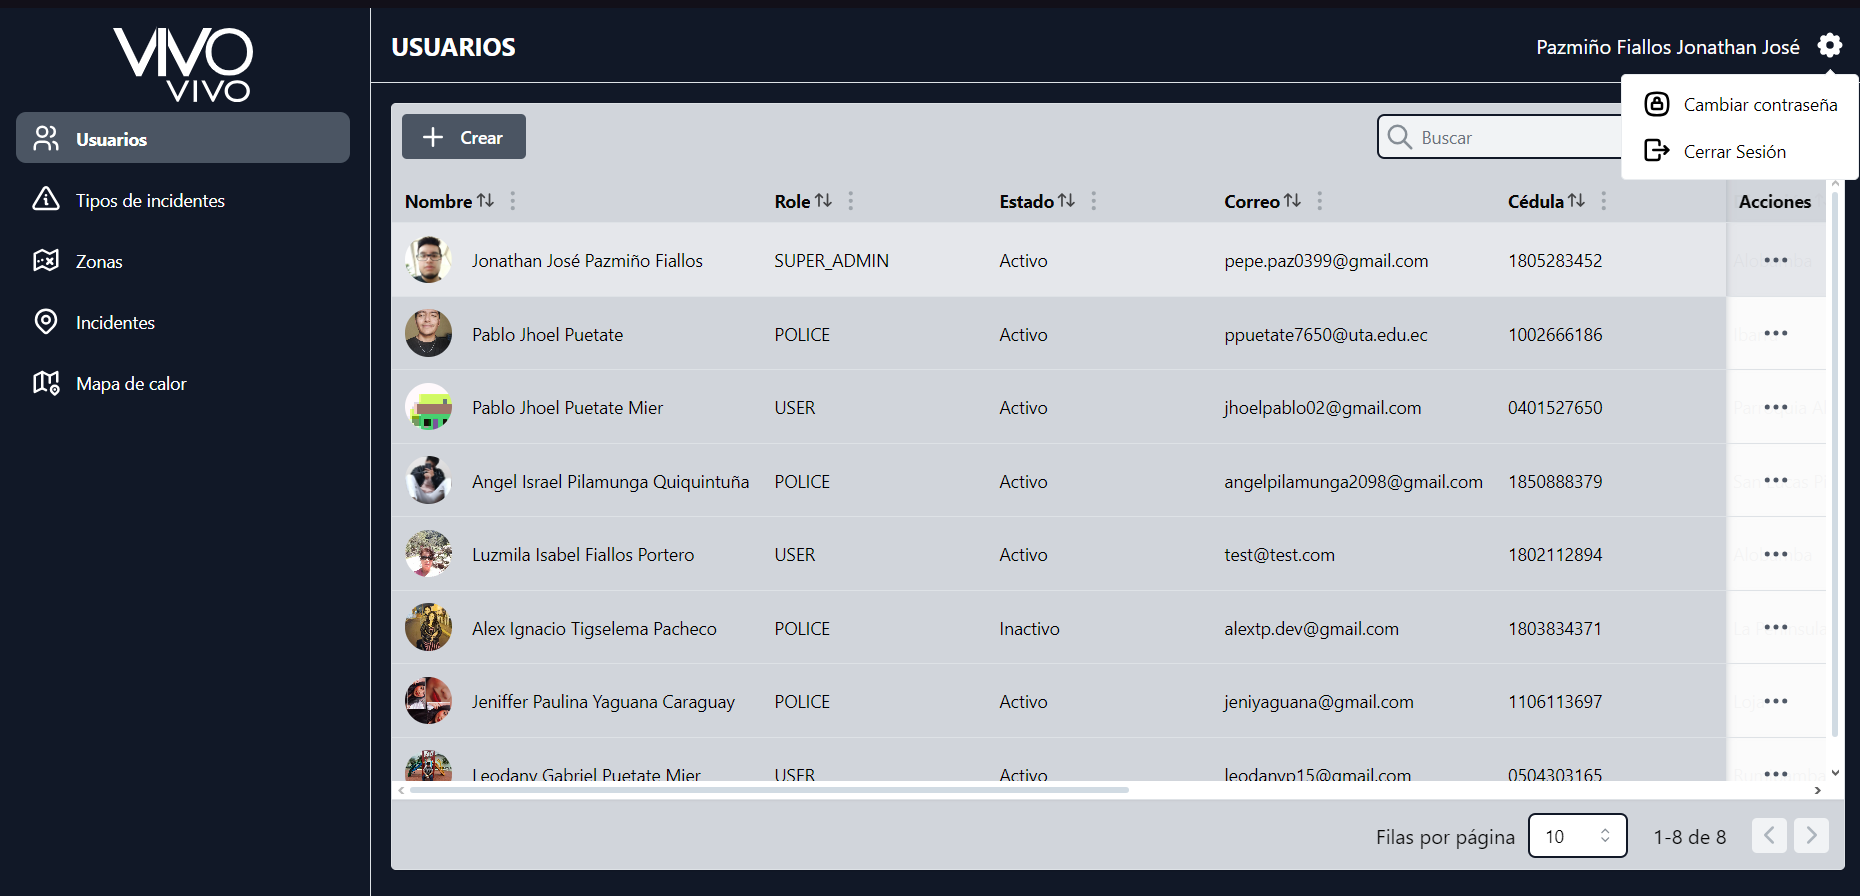
\includegraphics[width=0.8\textwidth]{chapters/III-resultados-y-discusion/resources/images/menu-usuario-web.png}
    \caption{Menú de usuario en el sistema web.}
    \label{fig:menu-usuario-web}
\end{figure}

\paragraph{Gestión de usuarios}
La gestión de usuarios en el sistema web se realiza mediante una tabla de entradas, la cual permite al usuario administrador
visualizar los usuarios registrados en el sistema, como se muestra en la Figura \ref{fig:tabla-usuarios-web}. En esta tabla se
muestran los campos de la información de los usuarios, como la fotografía, nombres, apellidos, correo electrónico, etnia, género,
entre otros. El usuario administrador puede realizar acciones como crear, editar y deshabilitar usuarios, como se puede observar en la Figura
\ref{fig:menu-tabla-usuarios-web}. El formulario de registro de usuarios permite al usuario administrador ingresar la información
necesaria para crear un nuevo usuario, como se puede visualizar en las Figuras \ref{fig:formulario-usuario-web-1} y \ref{fig:formulario-usuario-web-2}.

\begin{figure}[H]
    \centering
    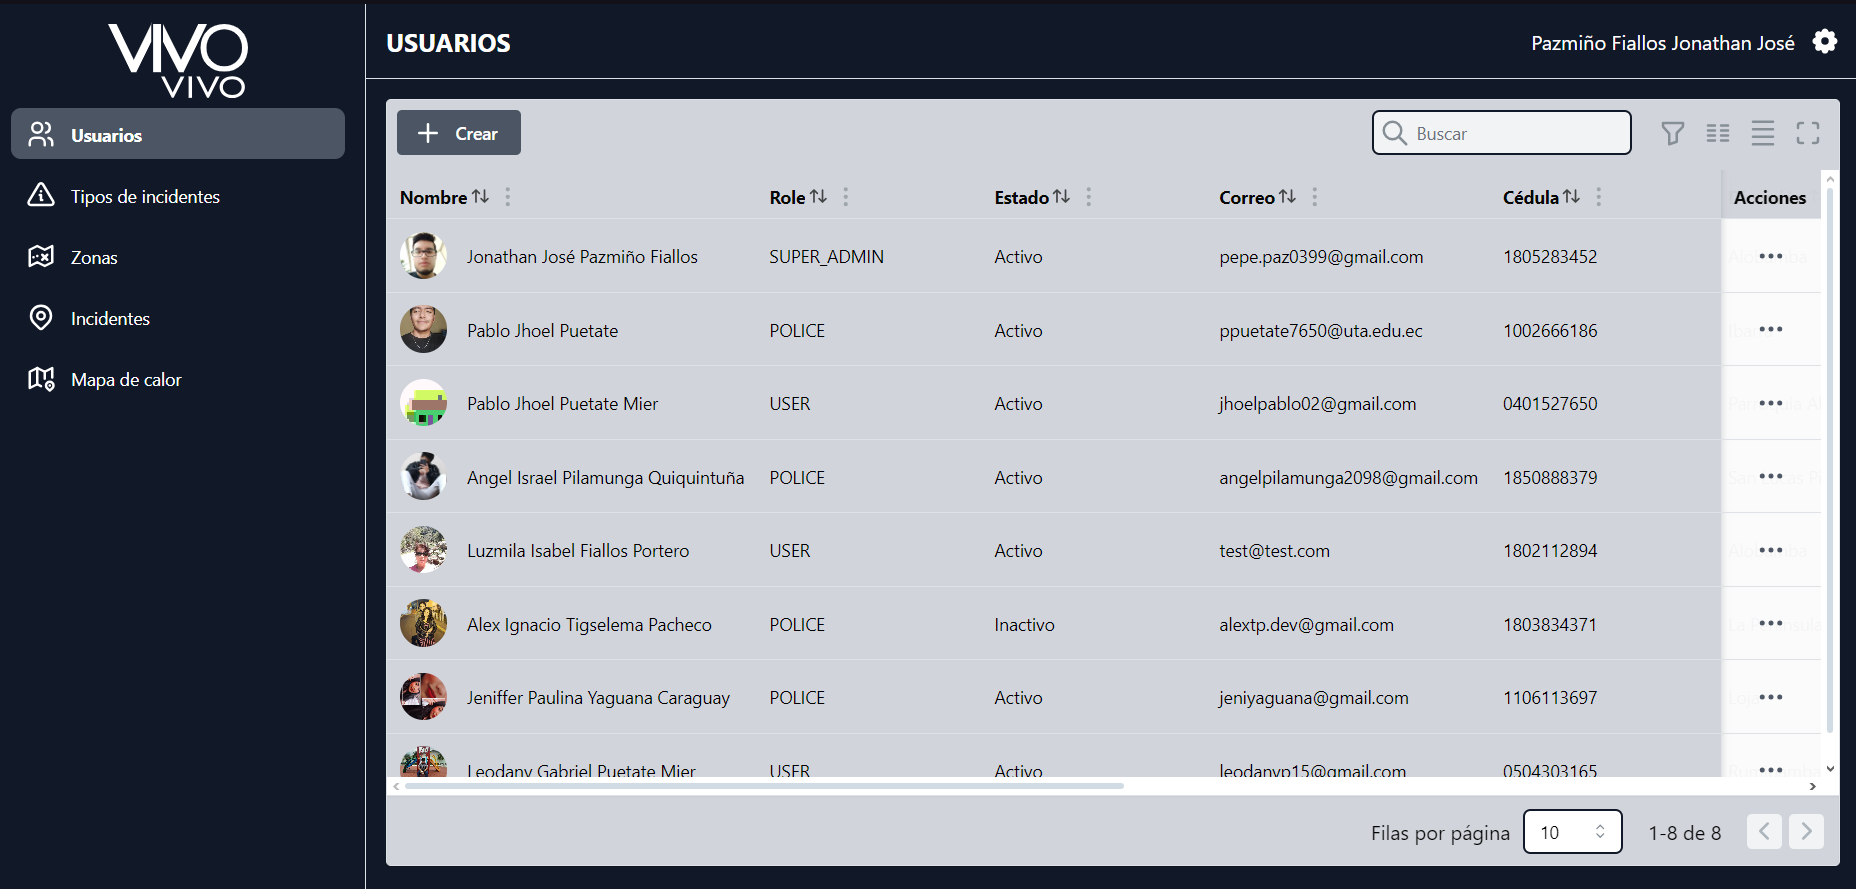
\includegraphics[width=0.8\textwidth]{chapters/III-resultados-y-discusion/resources/images/tabla-usuarios-web.png}
    \caption{Tabla de usuarios en el sistema web.}
    \label{fig:tabla-usuarios-web}
\end{figure}

\begin{figure}[H]
    \centering
    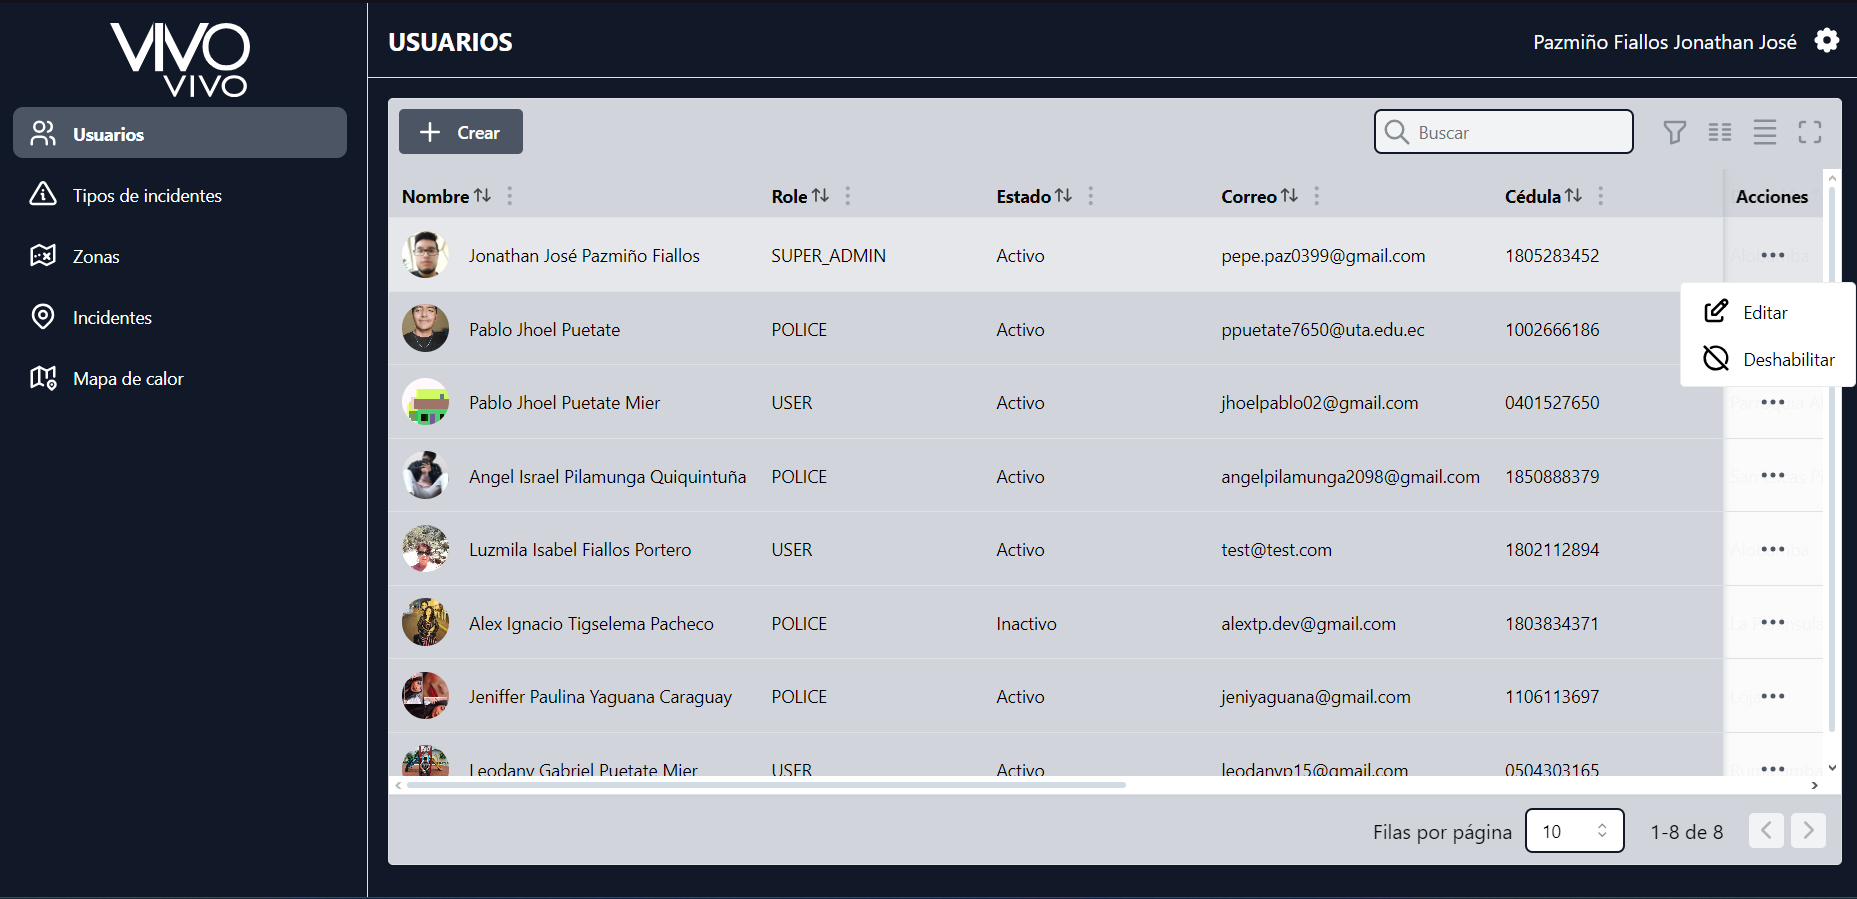
\includegraphics[width=0.8\textwidth]{chapters/III-resultados-y-discusion/resources/images/menu-tabla-usuarios-web.png}
    \caption{Menú de opciones de la tabla de usuarios en el sistema web.}
    \label{fig:menu-tabla-usuarios-web}
\end{figure}

\begin{figure}[H]
    \centering
    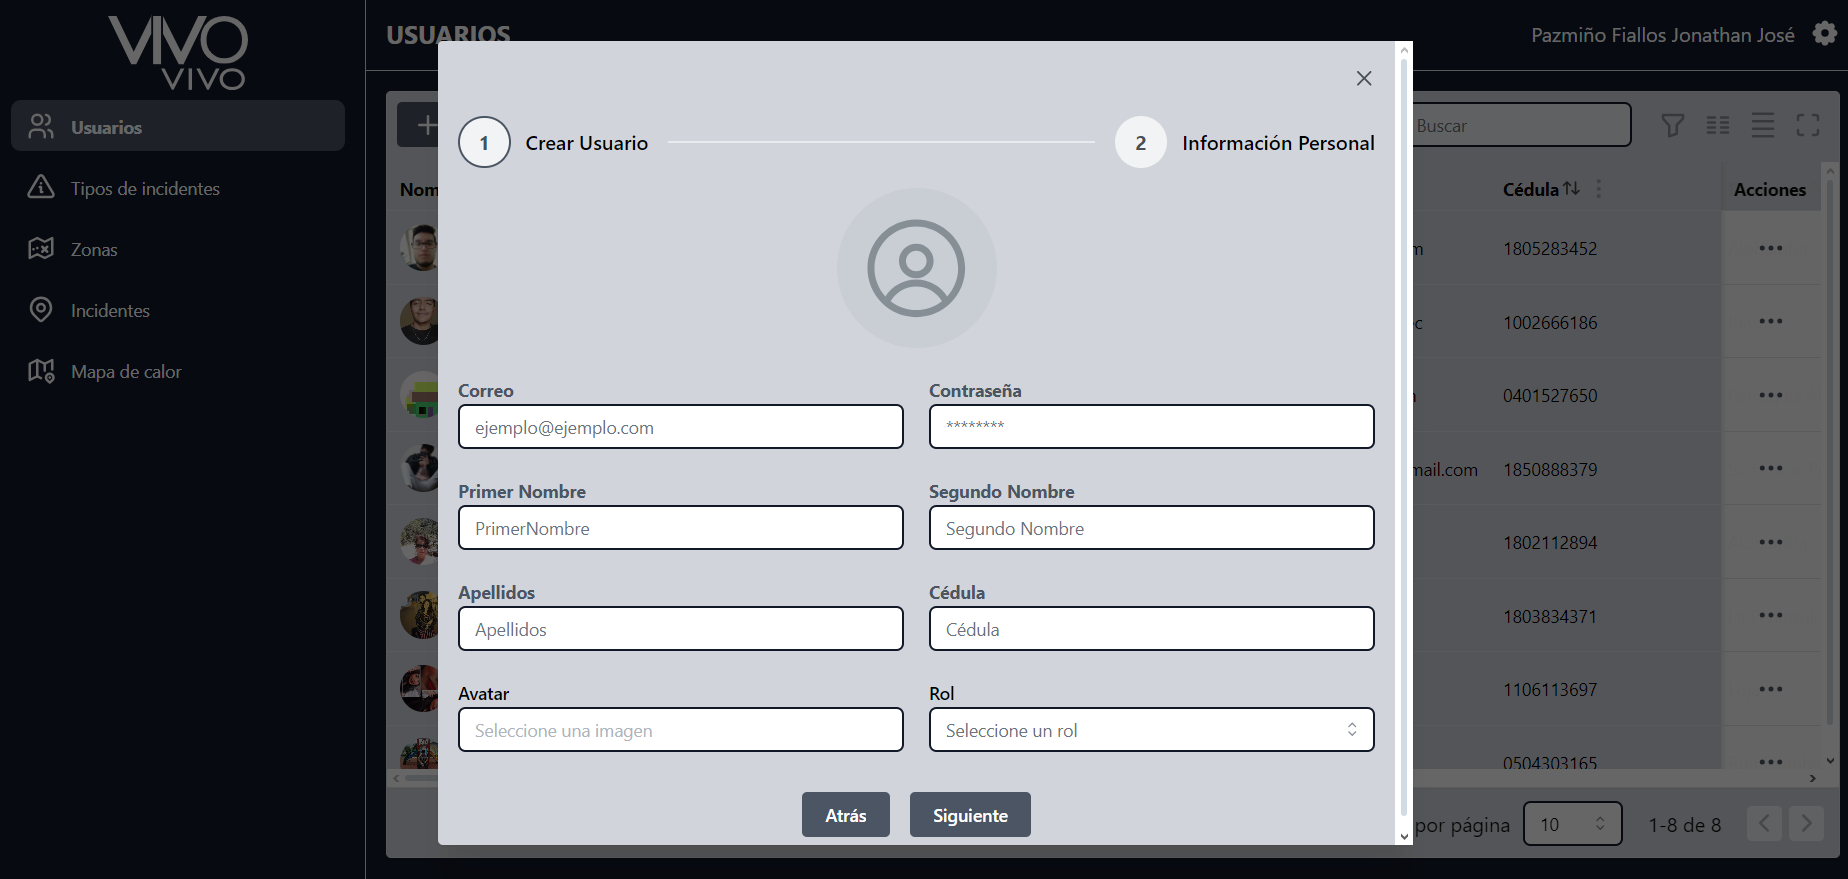
\includegraphics[width=0.8\textwidth]{chapters/III-resultados-y-discusion/resources/images/formulario-usuario-web-1.png}
    \caption{Formulario para crear/editar usuarios en el sistema web (Parte 1).}
    \label{fig:formulario-usuario-web-1}
\end{figure}

\begin{figure}[H]
    \centering
    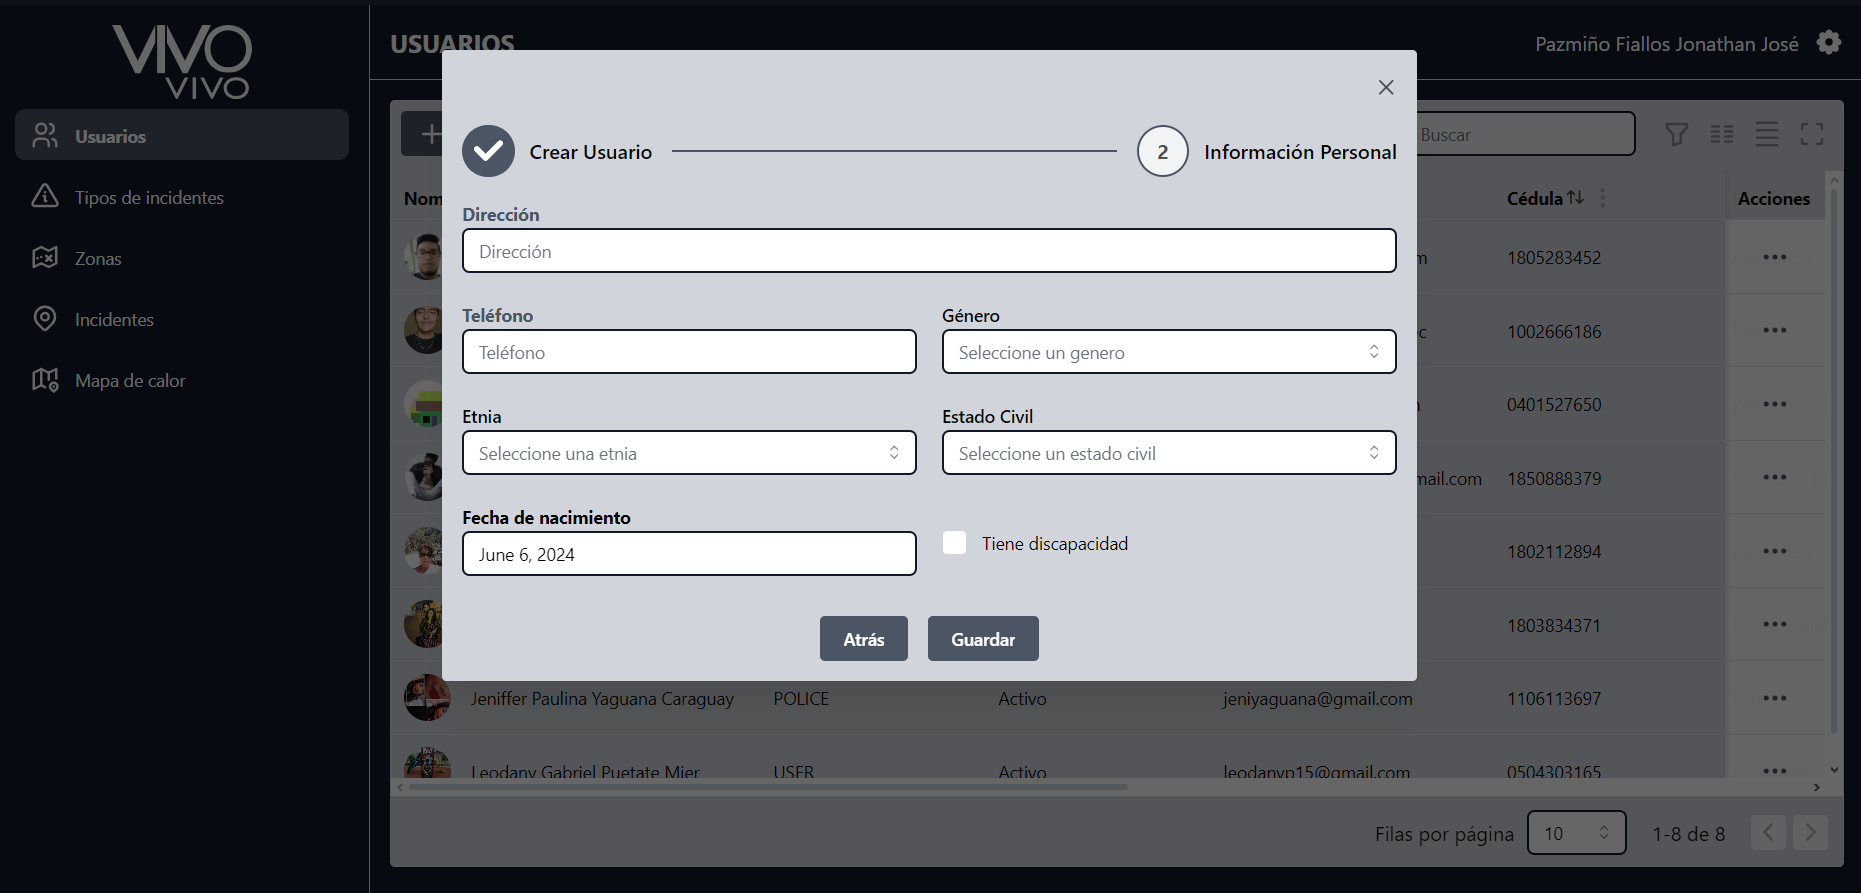
\includegraphics[width=0.8\textwidth]{chapters/III-resultados-y-discusion/resources/images/formulario-usuario-web-2.png}
    \caption{Formulario para crear/editar usuarios en el sistema web (Parte 2).}
    \label{fig:formulario-usuario-web-2}
\end{figure}

La tabla de gestión de usuarios cuenta con varios filtros de búsqueda, los cuales permiten al usuario administrador buscar usuarios por
columnas especificas o por un filtro general, como se muestra en la Figura \ref{fig:filtros-tabla-usuarios-web}.

\begin{figure}[H]
    \centering
    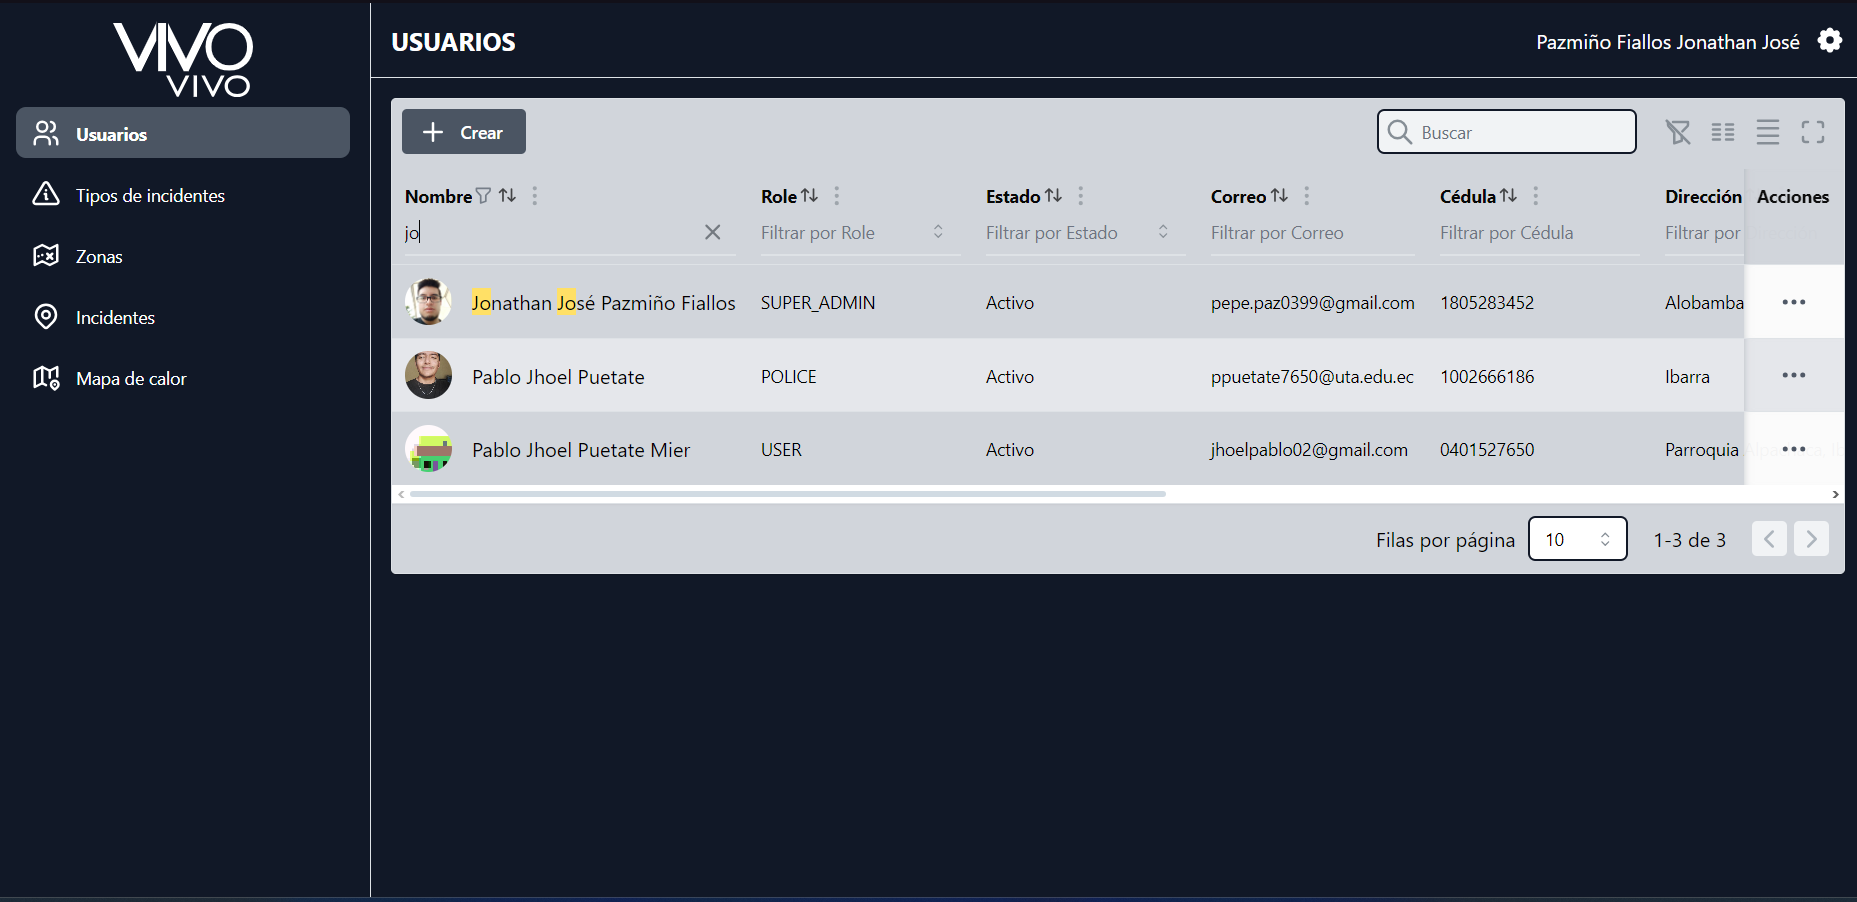
\includegraphics[width=0.8\textwidth]{chapters/III-resultados-y-discusion/resources/images/filtros-tabla-usuarios-web.png}
    \caption{Filtros de búsqueda en la tabla de usuarios en el sistema web.}
    \label{fig:filtros-tabla-usuarios-web}
\end{figure}

\paragraph{Gestión de tipos de incidentes}
La gestión de tipos de incidentes en el sistema web se realiza mediante una tabla de entradas, en la cual el usuario administrador
puede visualizar los tipos de incidentes registrados en el sistema, como se muestra en la Figura \ref{fig:tabla-tipos-incidentes-web}.
En esta tabla se muestran los campos de la información de los tipos de incidentes, como el nombre, descripción y estado. El usuario
administrador puede realizar acciones como crear, editar y deshabilitar tipos de incidentes, como se puede observar en la Figura
\ref{fig:menu-tabla-tipos-incidentes-web}. El formulario de registro de tipos de incidentes permite al usuario administrador ingresar
la información necesaria para crear un nuevo tipo de incidente, como se puede visualizar en la Figura \ref{fig:formulario-tipo-incidente-web}

\begin{figure}[H]
    \centering
    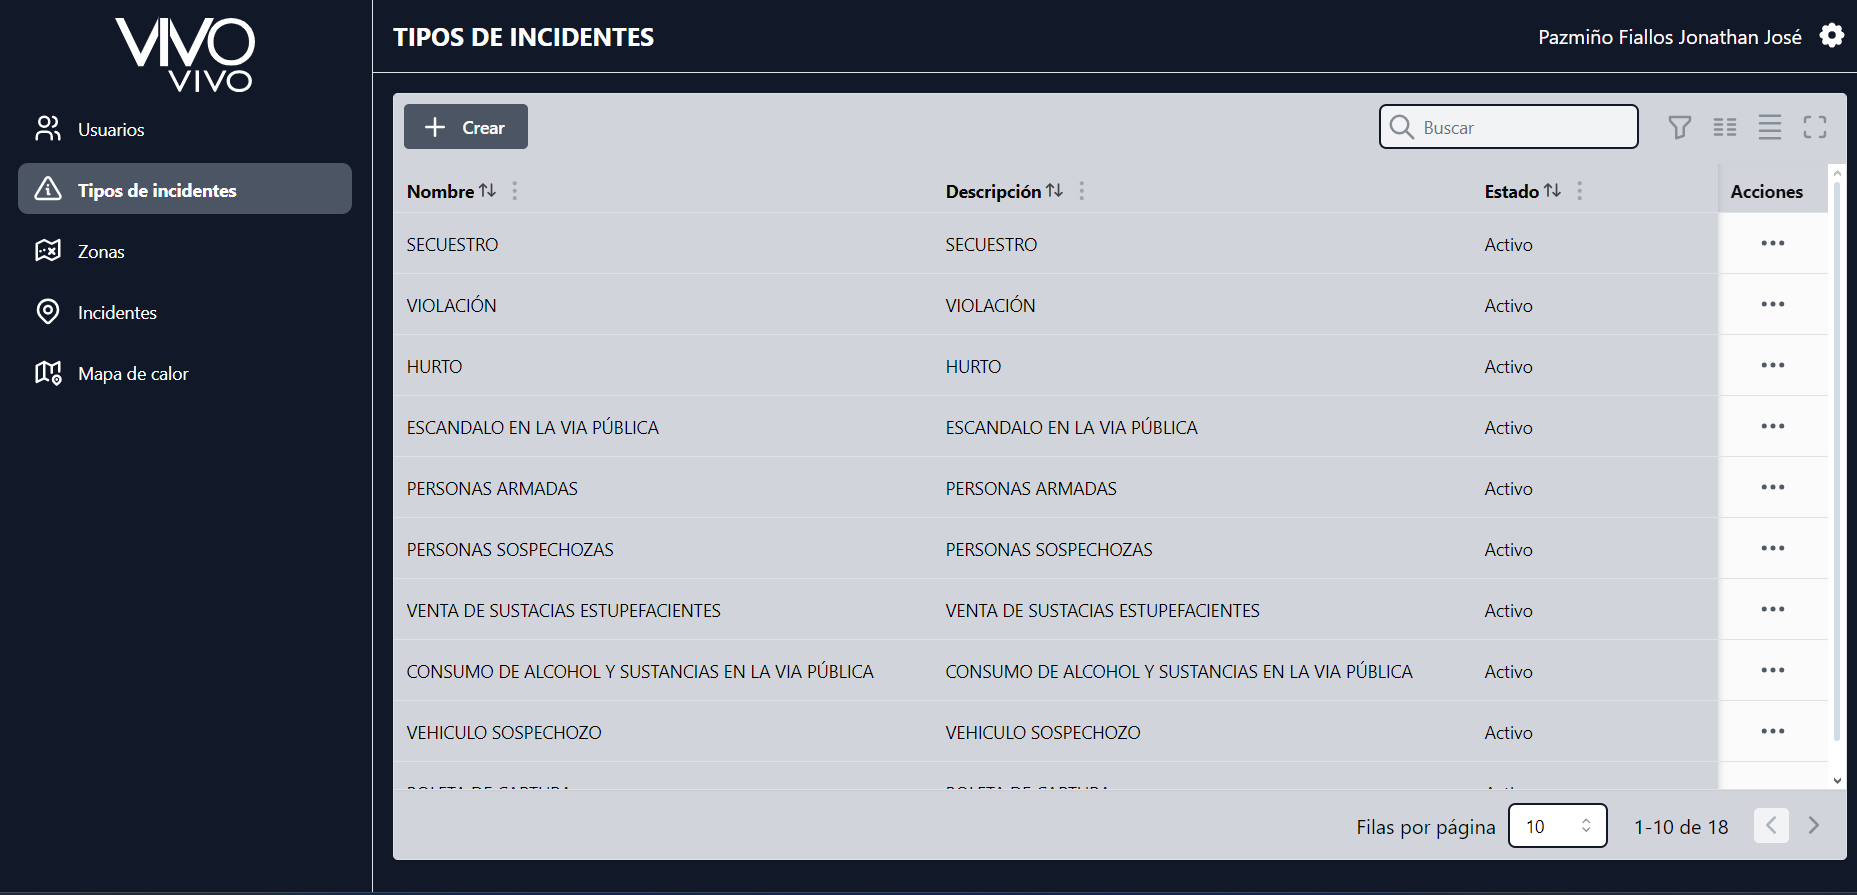
\includegraphics[width=0.8\textwidth]{chapters/III-resultados-y-discusion/resources/images/tabla-tipos-incidentes-web.png}
    \caption{Tabla de tipos de incidentes en el sistema web.}
    \label{fig:tabla-tipos-incidentes-web}
\end{figure}

\begin{figure}[H]
    \centering
    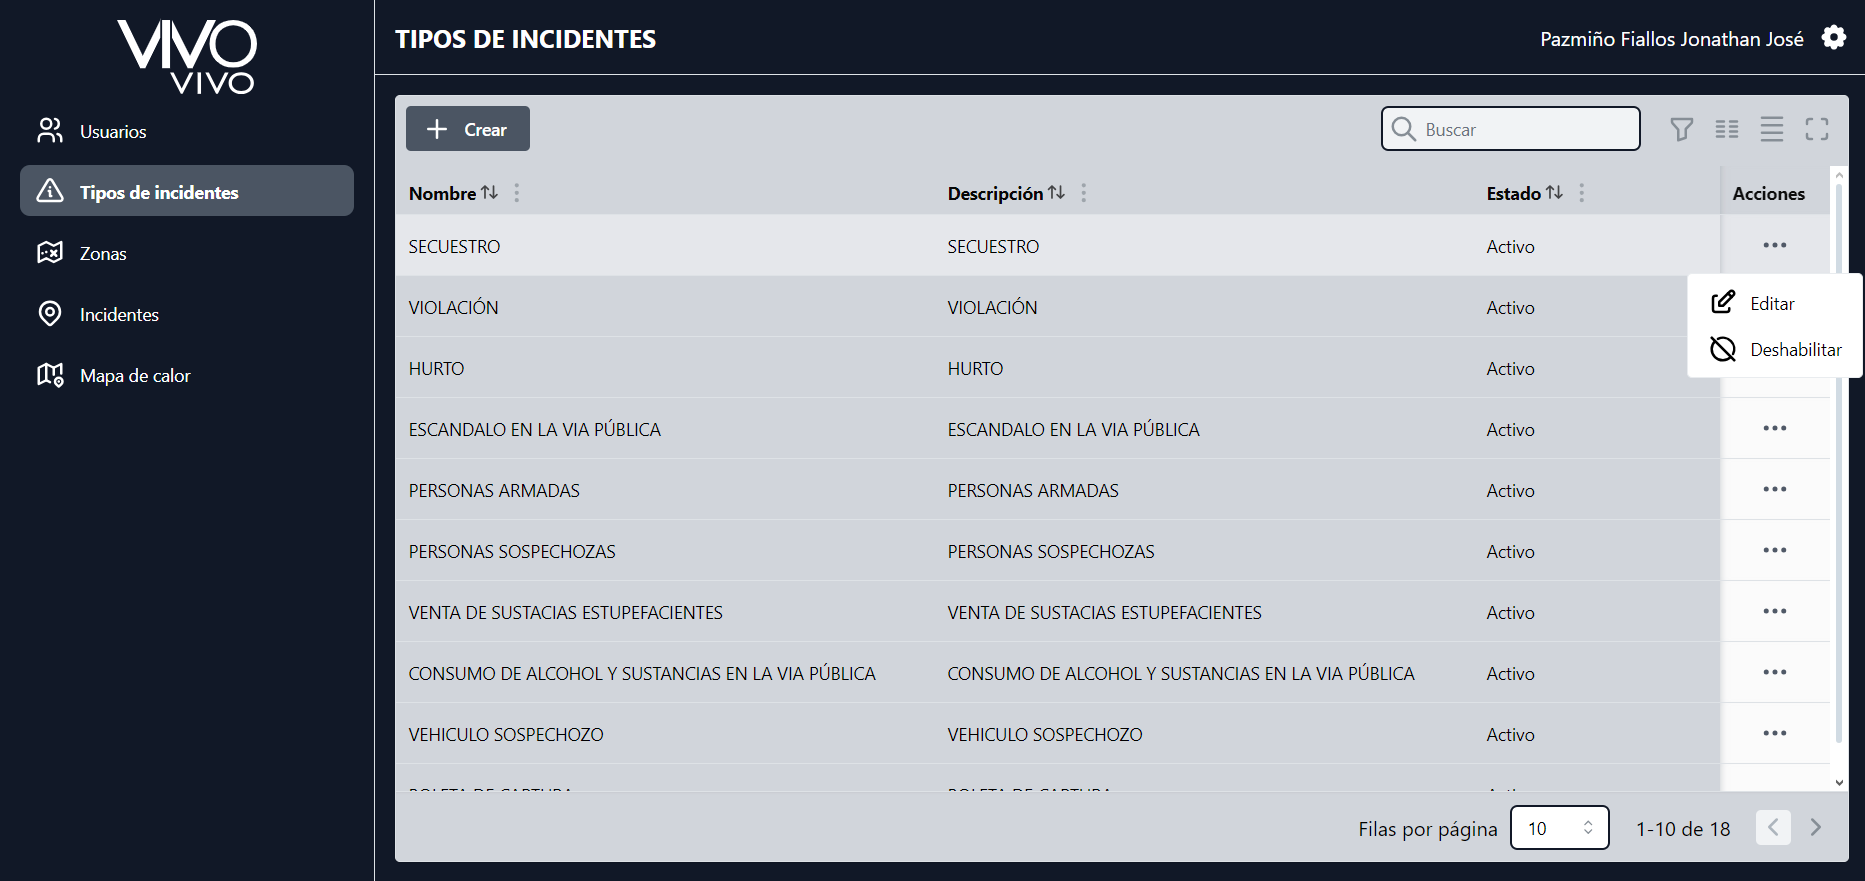
\includegraphics[width=0.8\textwidth]{chapters/III-resultados-y-discusion/resources/images/menu-tabla-tipos-incidentes-web.png}
    \caption{Menú de opciones de la tabla de tipos de incidentes en el sistema web.}
    \label{fig:menu-tabla-tipos-incidentes-web}
\end{figure}

\begin{figure}[H]
    \centering
    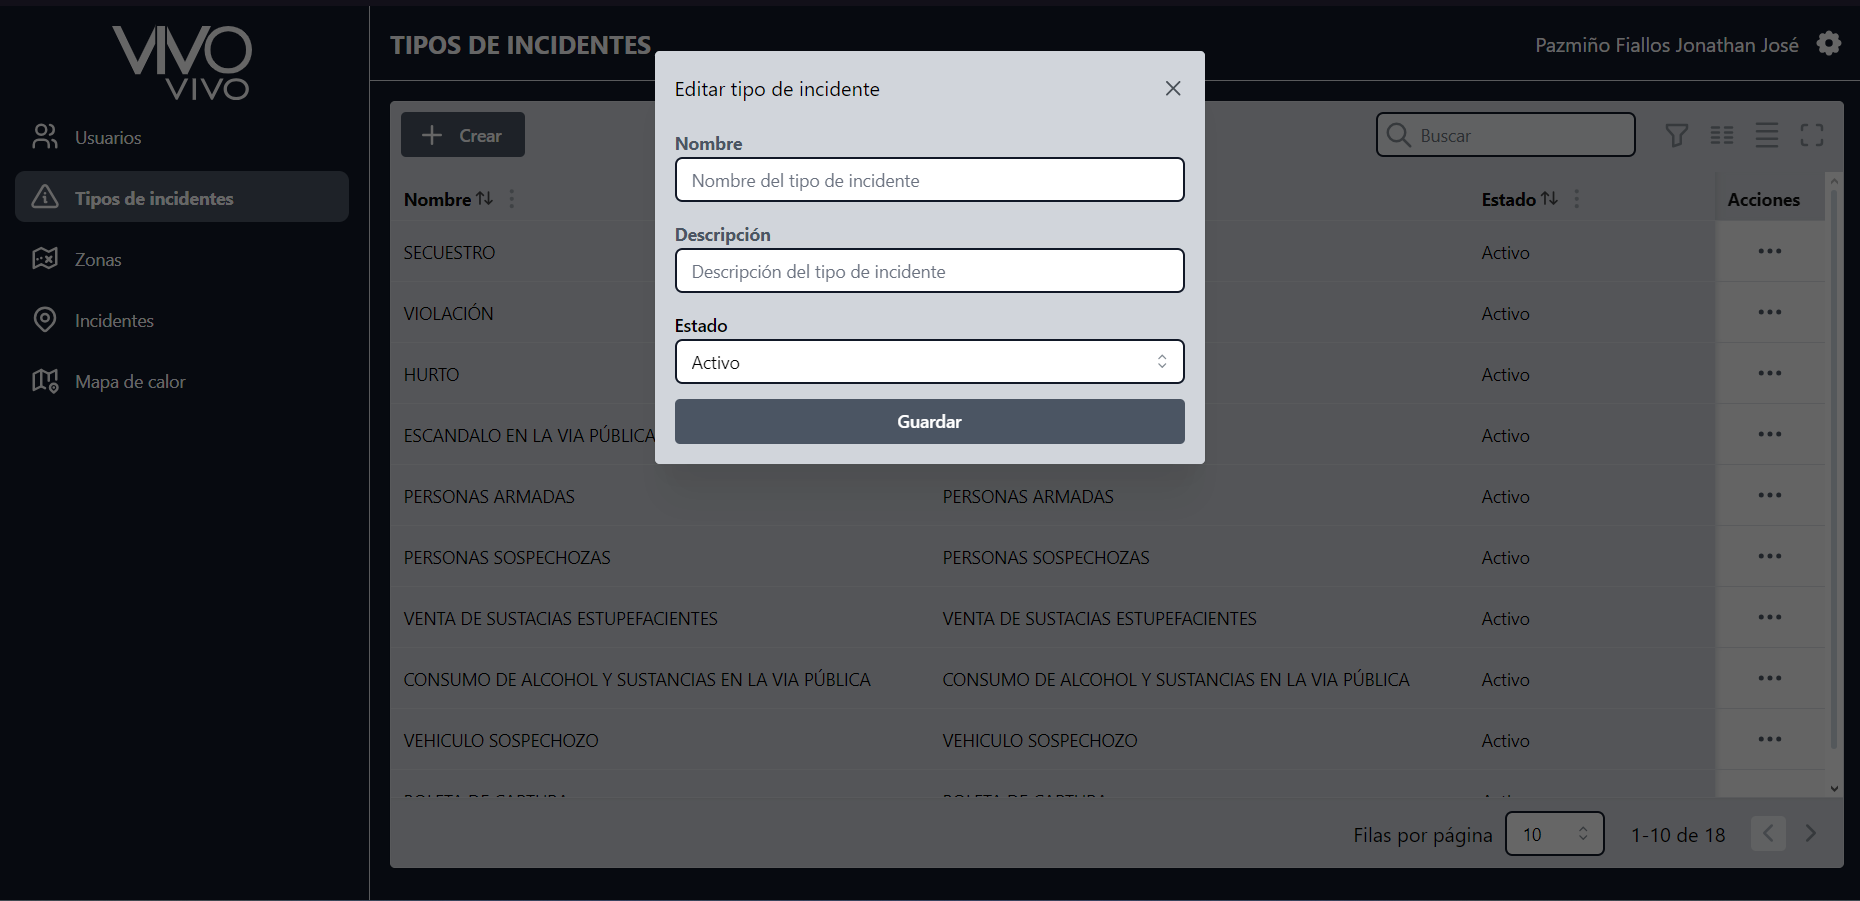
\includegraphics[width=0.8\textwidth]{chapters/III-resultados-y-discusion/resources/images/formulario-tipo-incidente-web.png}
    \caption{Formulario para crear/editar tipos de incidentes en el sistema web.}
    \label{fig:formulario-tipo-incidente-web}
\end{figure}

La tabla de gestión de tipos de incidentes cuenta con varios filtros de búsqueda, los cuales permiten al usuario administrador buscar
tipos de incidentes por columnas especificas o por un filtro general, como se muestra en la Figura \ref{fig:filtros-tabla-tipos-incidentes-web}.

\begin{figure}[H]
    \centering
    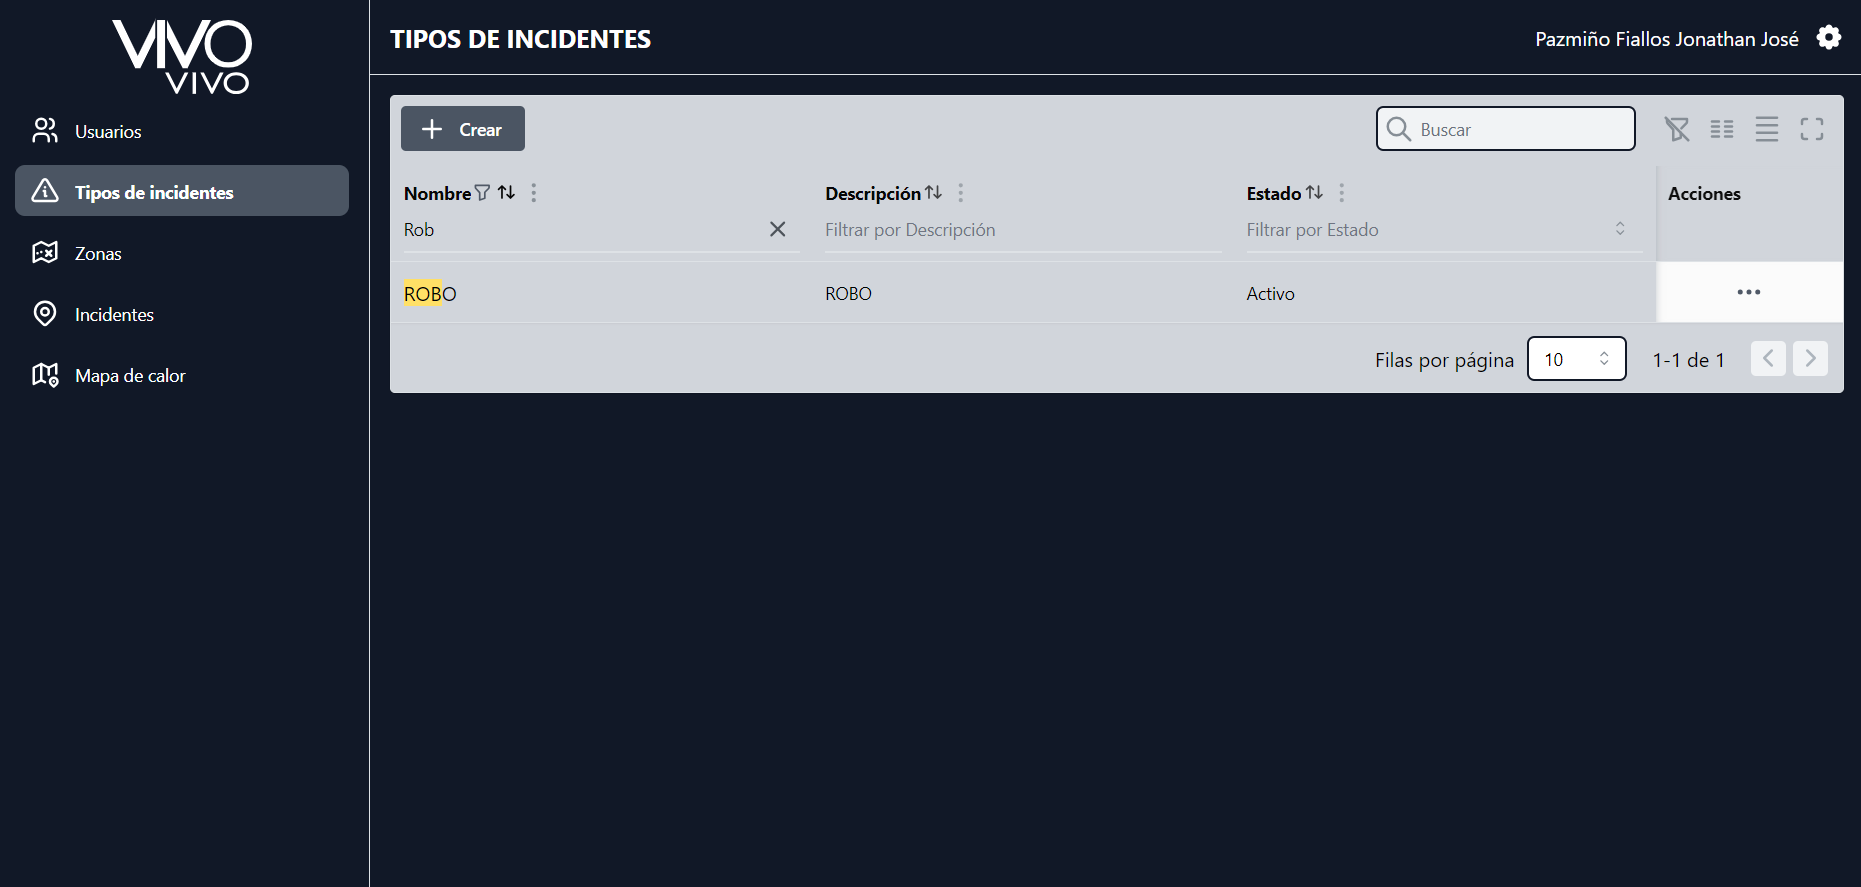
\includegraphics[width=0.8\textwidth]{chapters/III-resultados-y-discusion/resources/images/filtros-tabla-tipos-incidentes-web.png}
    \caption{Filtros de búsqueda en la tabla de tipos de incidentes en el sistema web.}
    \label{fig:filtros-tabla-tipos-incidentes-web}
\end{figure}

\paragraph{Gestión de zonas de vigilancia}

La gestión de zonas de vigilancia en el sistema web se realiza por medio de un mapa interactivo, en el cual el usuario administrador
puede visualizar las zonas de vigilancia mediante polígonos, como se muestra en la Figura \ref{fig:mapa-zonas-vigilancia-web}.
El usuario administrador puede realizar acciones como crear, editar y deshabilitar zonas de vigilancia, como se puede observar en la Figura
\ref{fig:menu-mapa-zonas-vigilancia-web}. El formulario de registro de zonas de vigilancia permite al usuario administrador dibujar
un polígono en el mapa para definir una zona de vigilancia, como se puede visualizar en la Figura \ref{fig:formulario-zona-vigilancia-web}.
Además, el usuario administrador podrá asignar policías a las zonas de vigilancia, como se muestra en la Figura
\ref{fig:asignar-policias-zona-vigilancia-web}.

\begin{figure}[H]
    \centering
    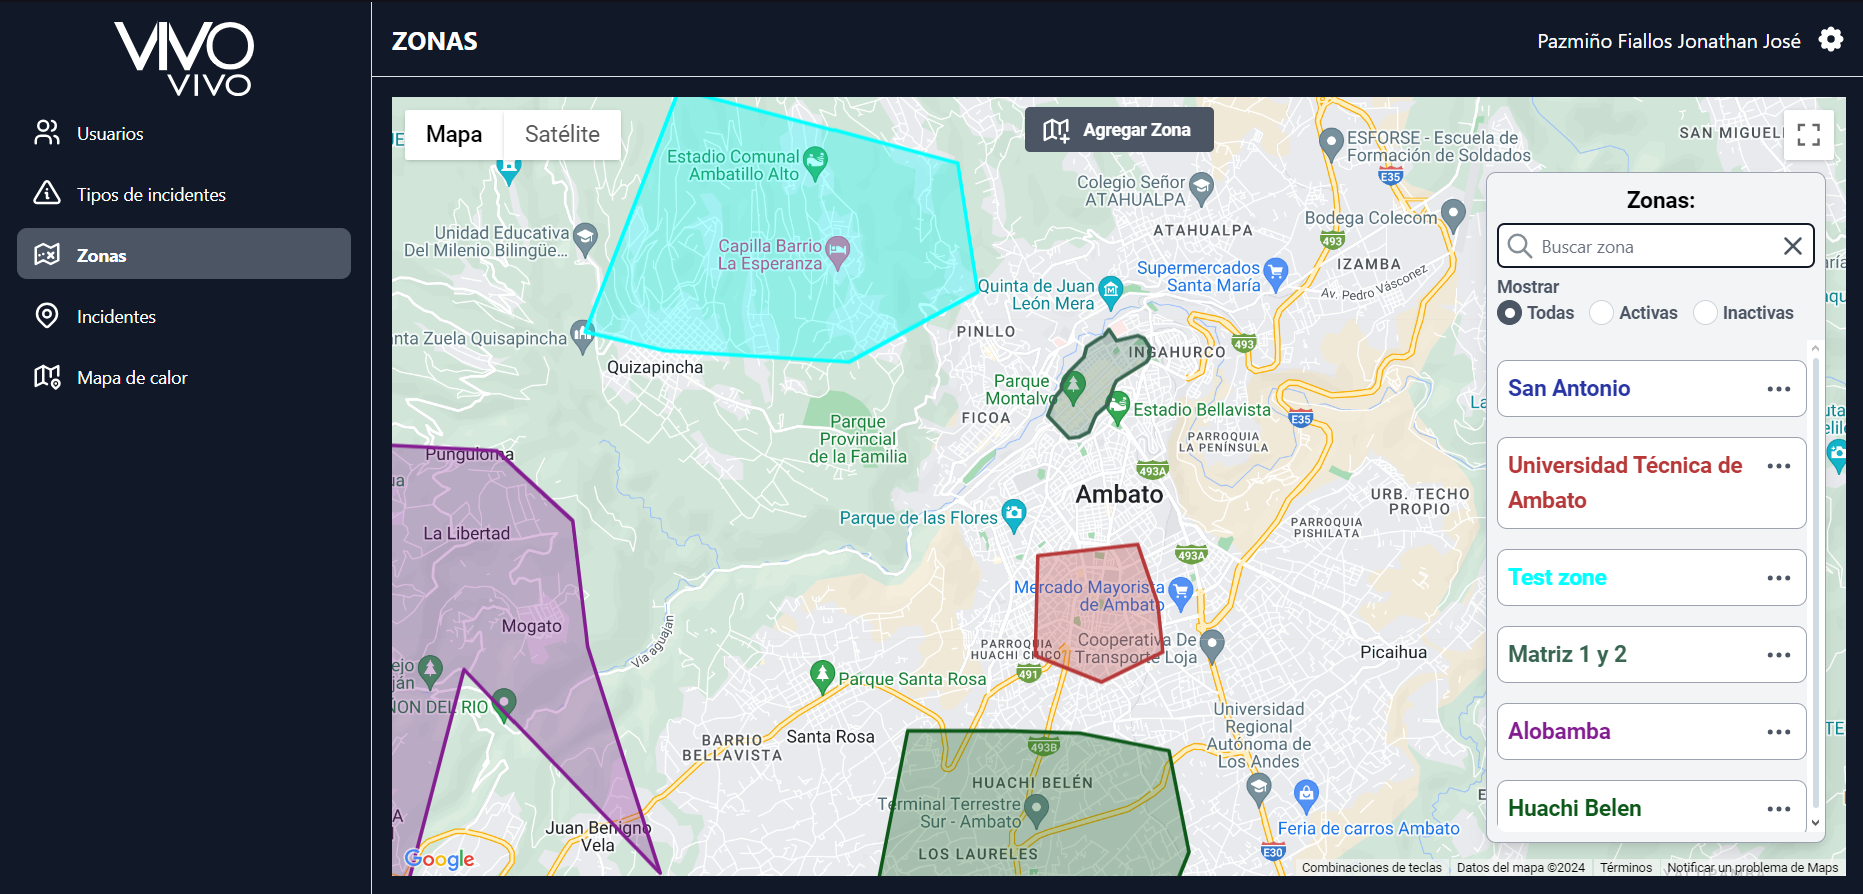
\includegraphics[width=0.8\textwidth]{chapters/III-resultados-y-discusion/resources/images/mapa-zonas-vigilancia-web.png}
    \caption{Mapa de zonas de vigilancia en el sistema web.}
    \label{fig:mapa-zonas-vigilancia-web}
\end{figure}

\begin{figure}[H]
    \centering
    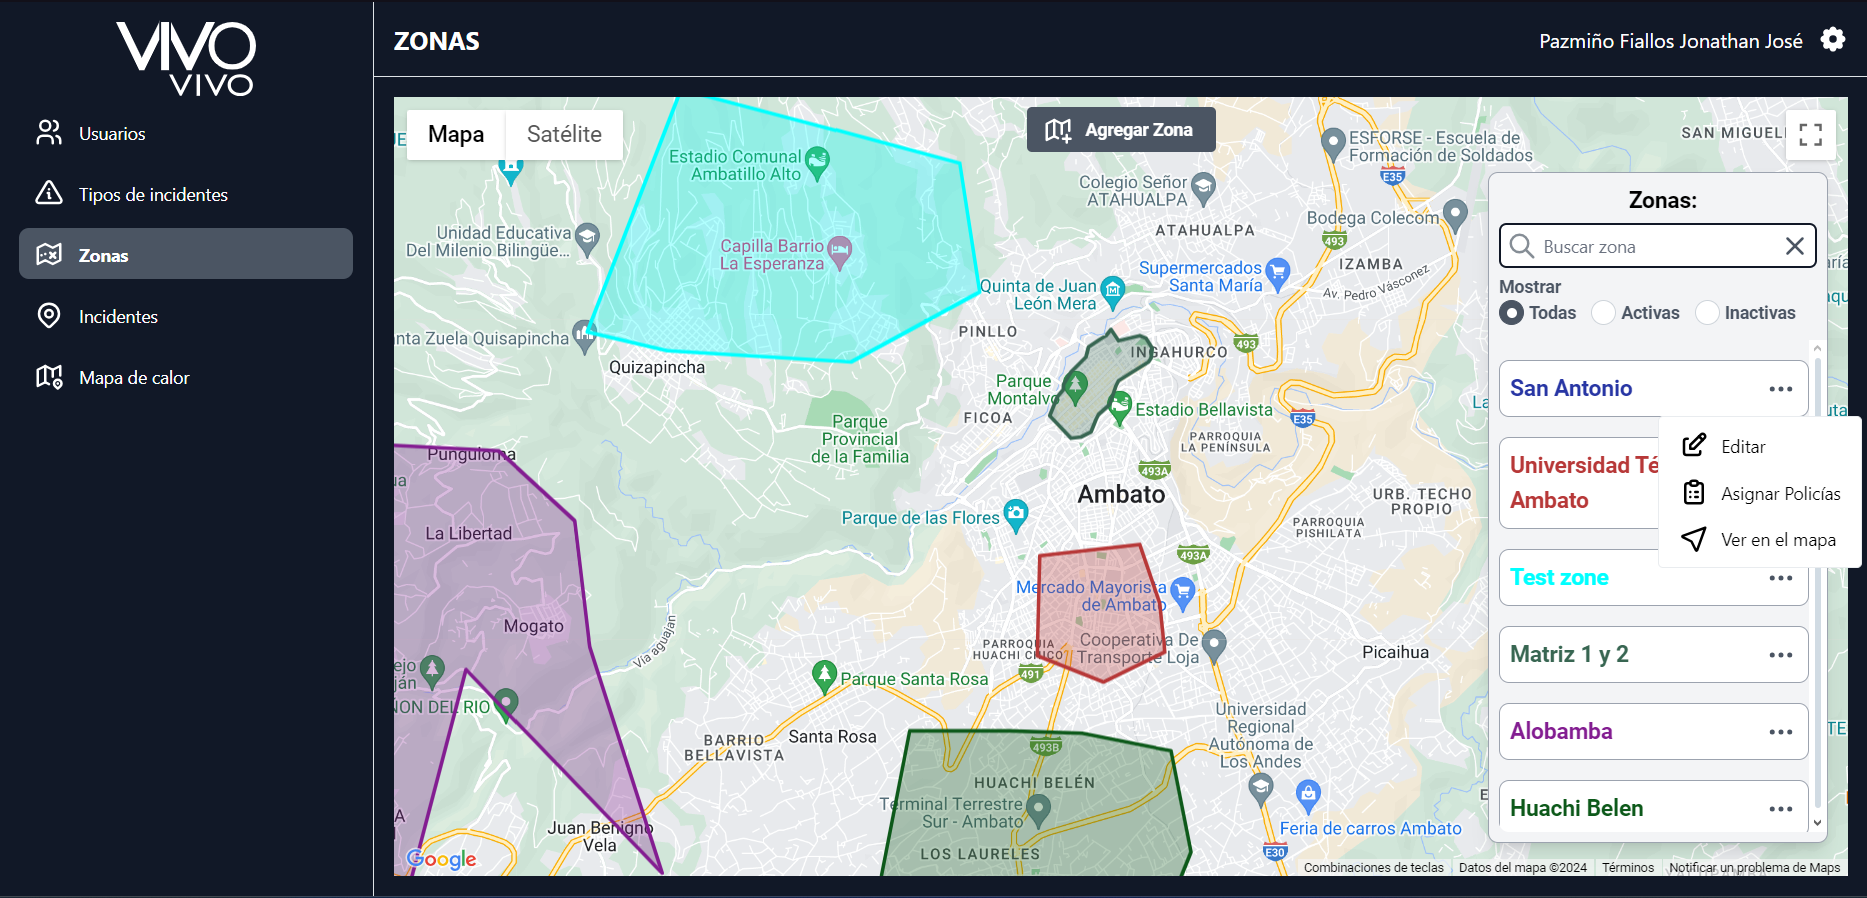
\includegraphics[width=0.8\textwidth]{chapters/III-resultados-y-discusion/resources/images/menu-mapa-zonas-vigilancia-web.png}
    \caption{Menú de opciones del mapa de zonas de vigilancia en el sistema web.}
    \label{fig:menu-mapa-zonas-vigilancia-web}
\end{figure}

\begin{figure}[H]
    \centering
    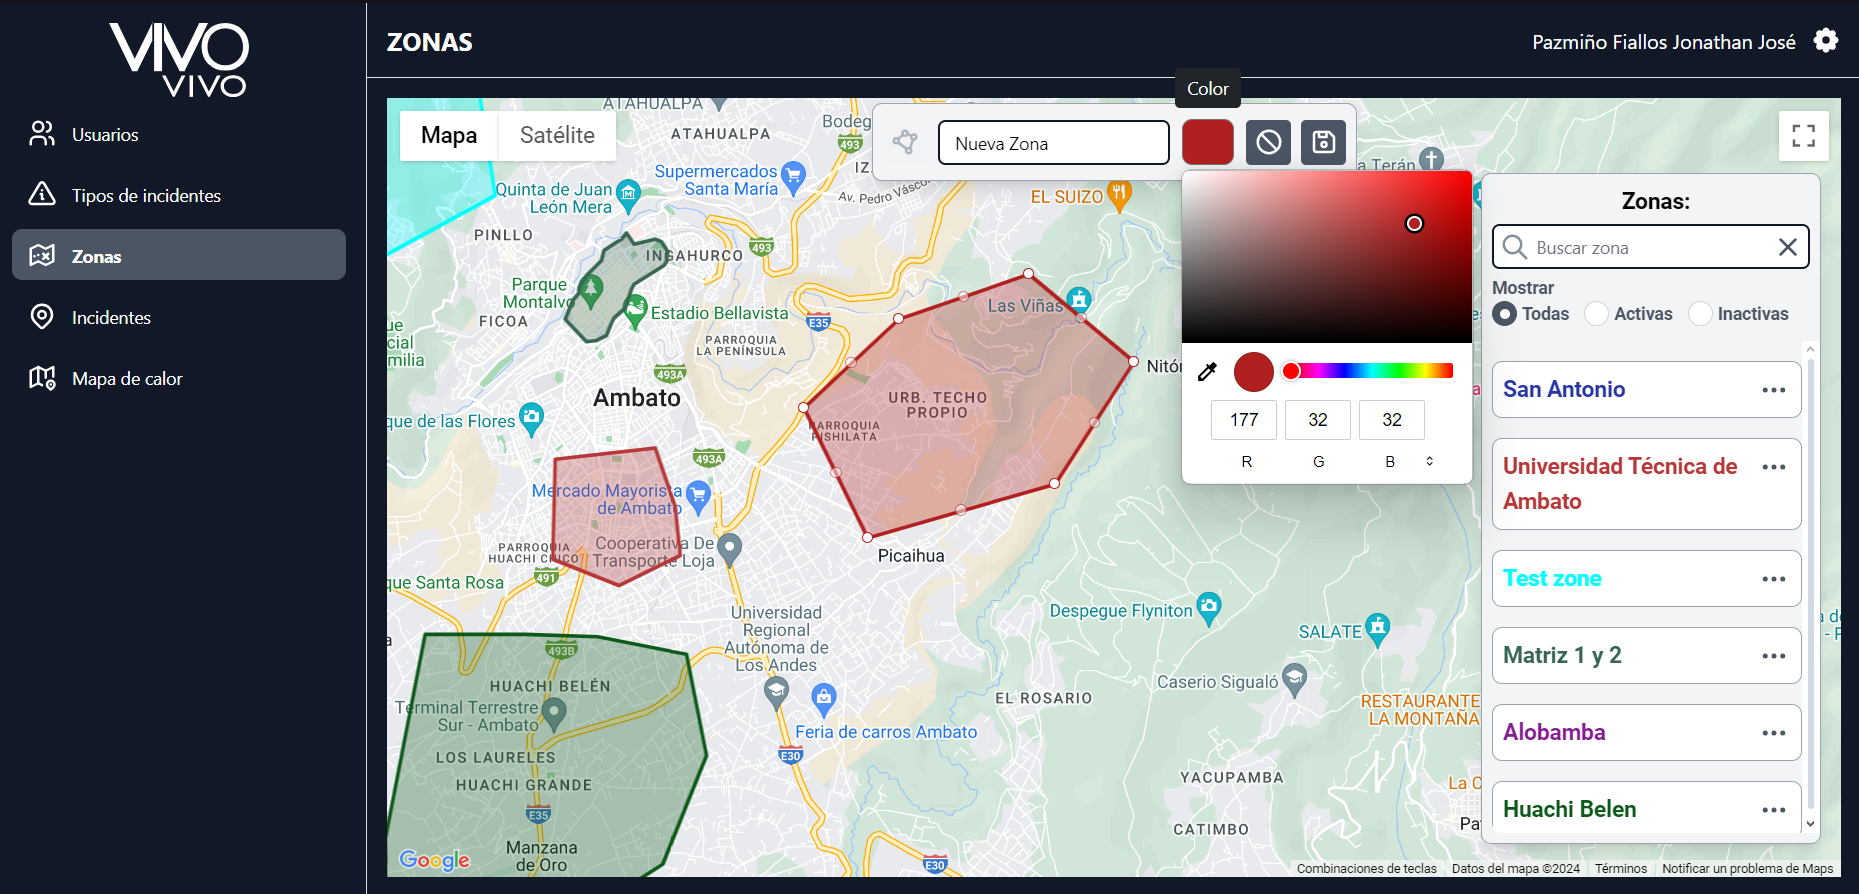
\includegraphics[width=0.8\textwidth]{chapters/III-resultados-y-discusion/resources/images/formulario-zona-vigilancia-web.png}
    \caption{Formulario para crear/editar zonas de vigilancia en el sistema web.}
    \label{fig:formulario-zona-vigilancia-web}
\end{figure}

\begin{figure}[H]
    \centering
    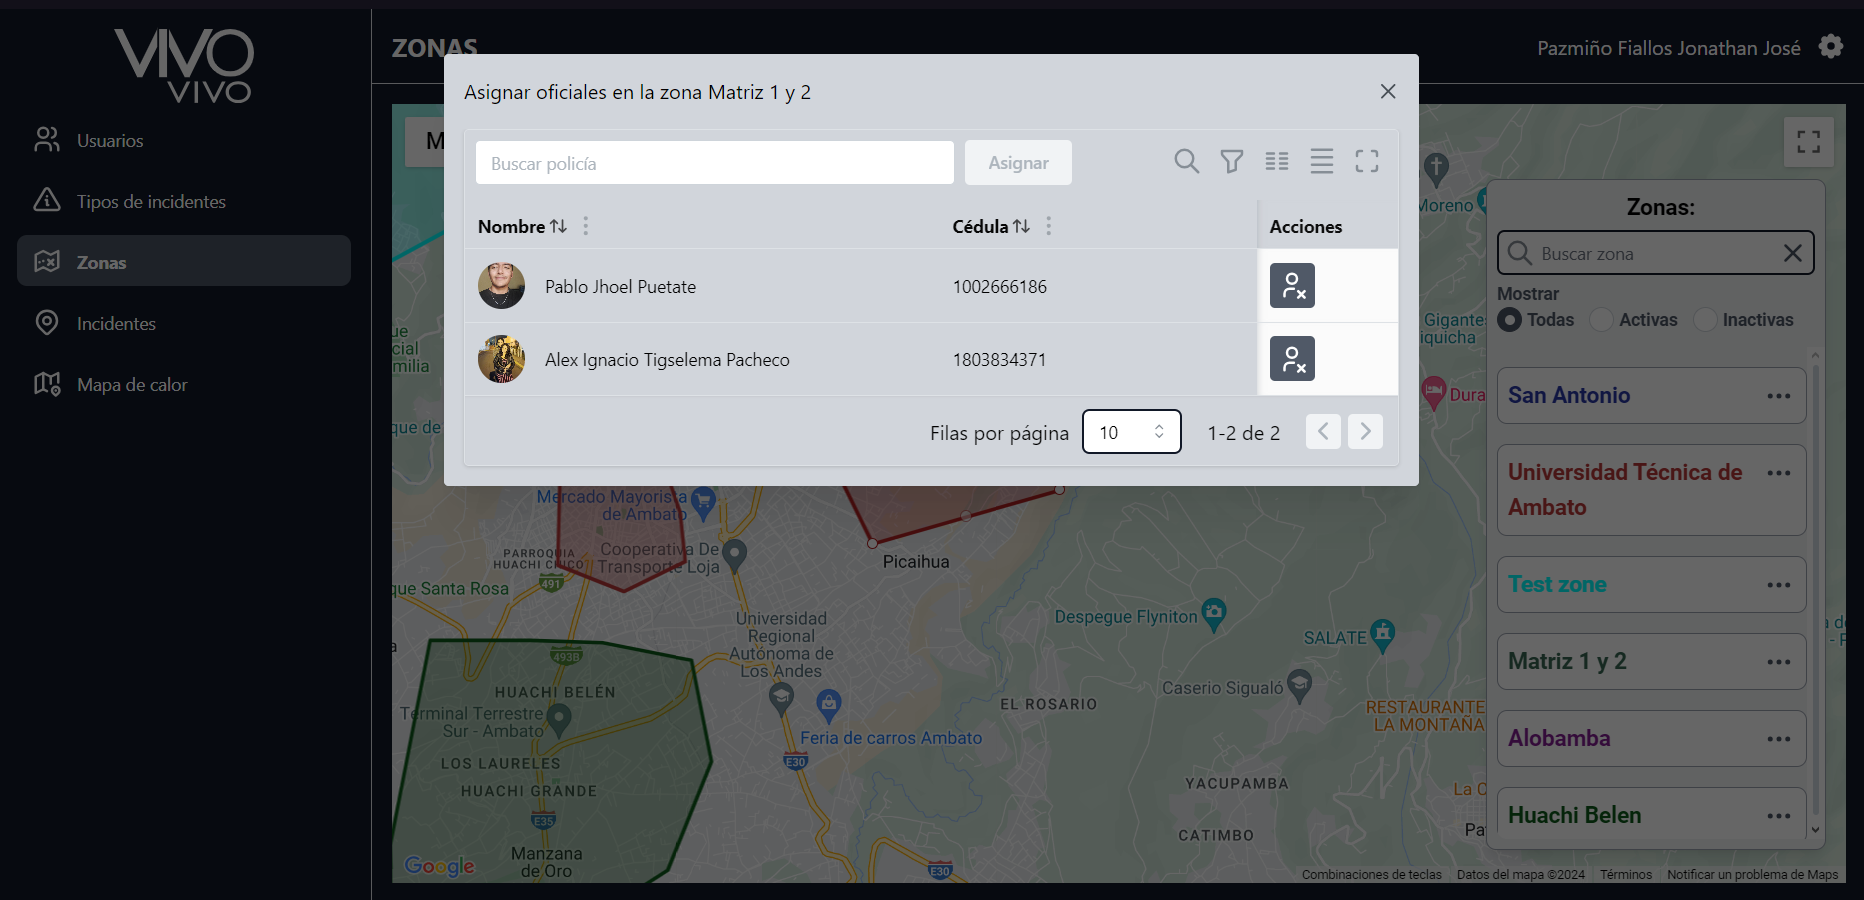
\includegraphics[width=0.8\textwidth]{chapters/III-resultados-y-discusion/resources/images/asignar-policias-zona-vigilancia-web.png}
    \caption{Asignar policías a zonas de vigilancia en el sistema web.}
    \label{fig:asignar-policias-zona-vigilancia-web}
\end{figure}

\paragraph{Gestión de incidentes}
La gestión de incidentes en el sistema web se realiza empleando un mapa interactivo, en el cual el usuario administrador puede visualizar
los incidentes reportados junto con la ubicación en tiempo real de la víctima, así como la ubicación de los policías en la zona de emergencia,
como se muestra en la Figura \ref{fig:mapa-incidentes-web}. El usuario administrador podrá visualizar el tipo de incidente y modificarlo en
caso de ser necesario. Además, podrá visualizar información de la víctima y de los policías asignados, como se puede observar en la Figura
\ref{fig:detalles-incidente-web}.

\begin{figure}[H]
    \centering
    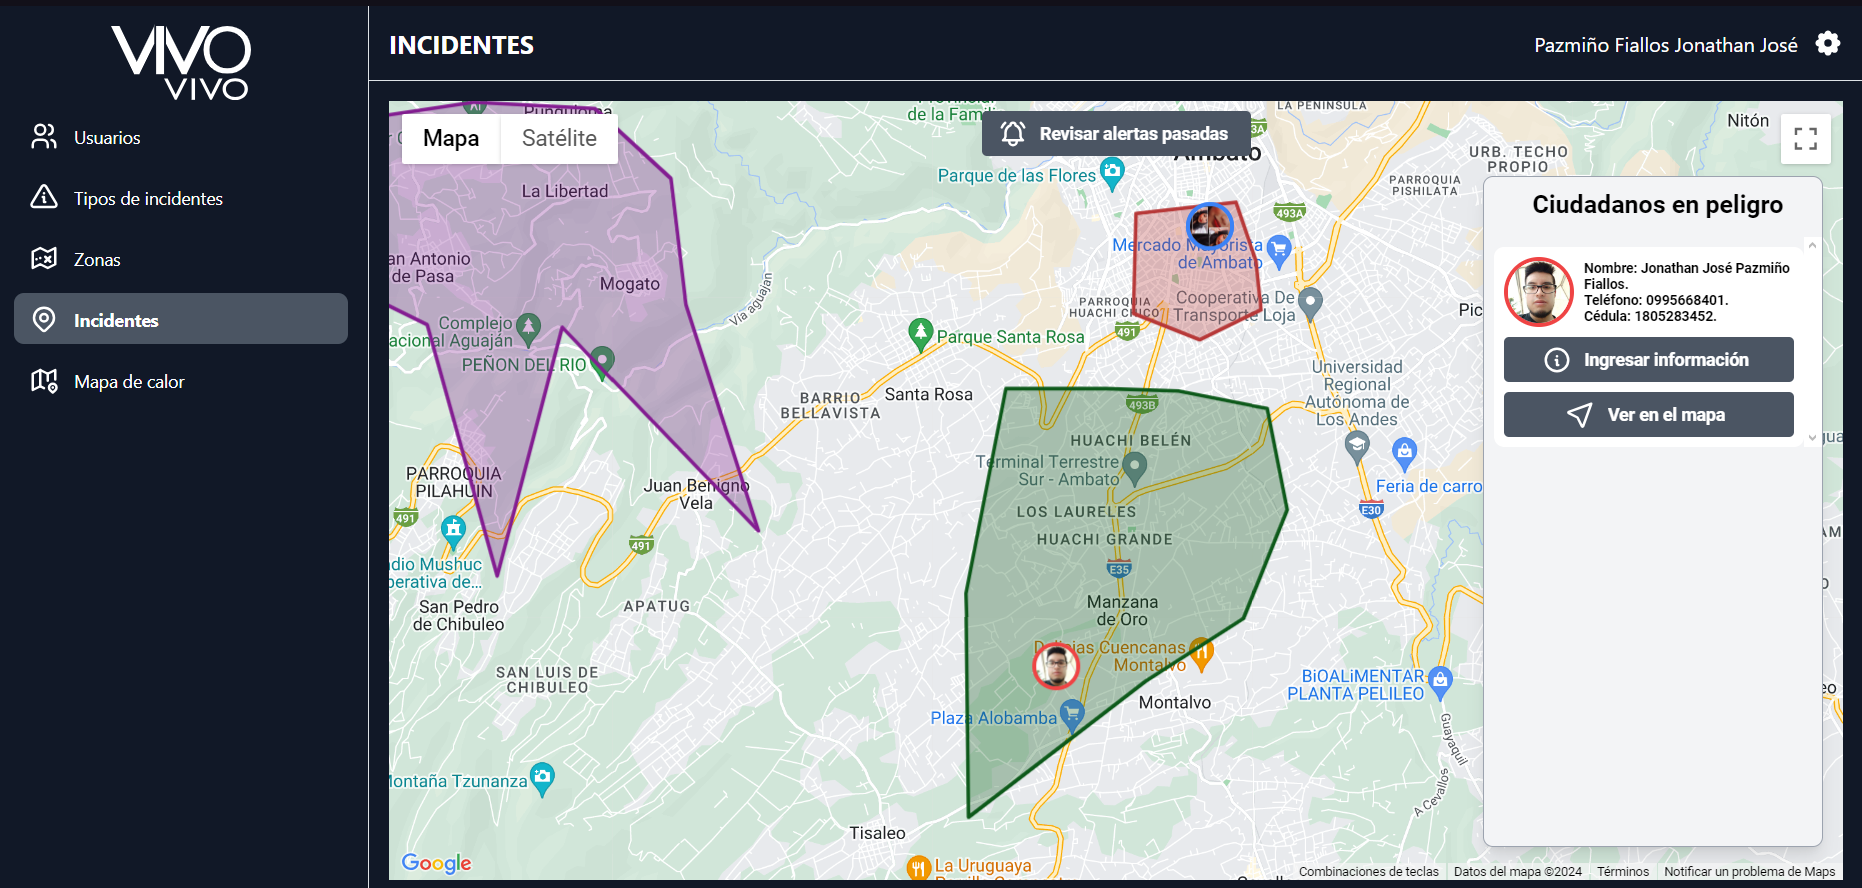
\includegraphics[width=0.8\textwidth]{chapters/III-resultados-y-discusion/resources/images/mapa-incidentes-web.png}
    \caption{Mapa de incidentes en el sistema web.}
    \label{fig:mapa-incidentes-web}
\end{figure}

\begin{figure}[H]
    \centering
    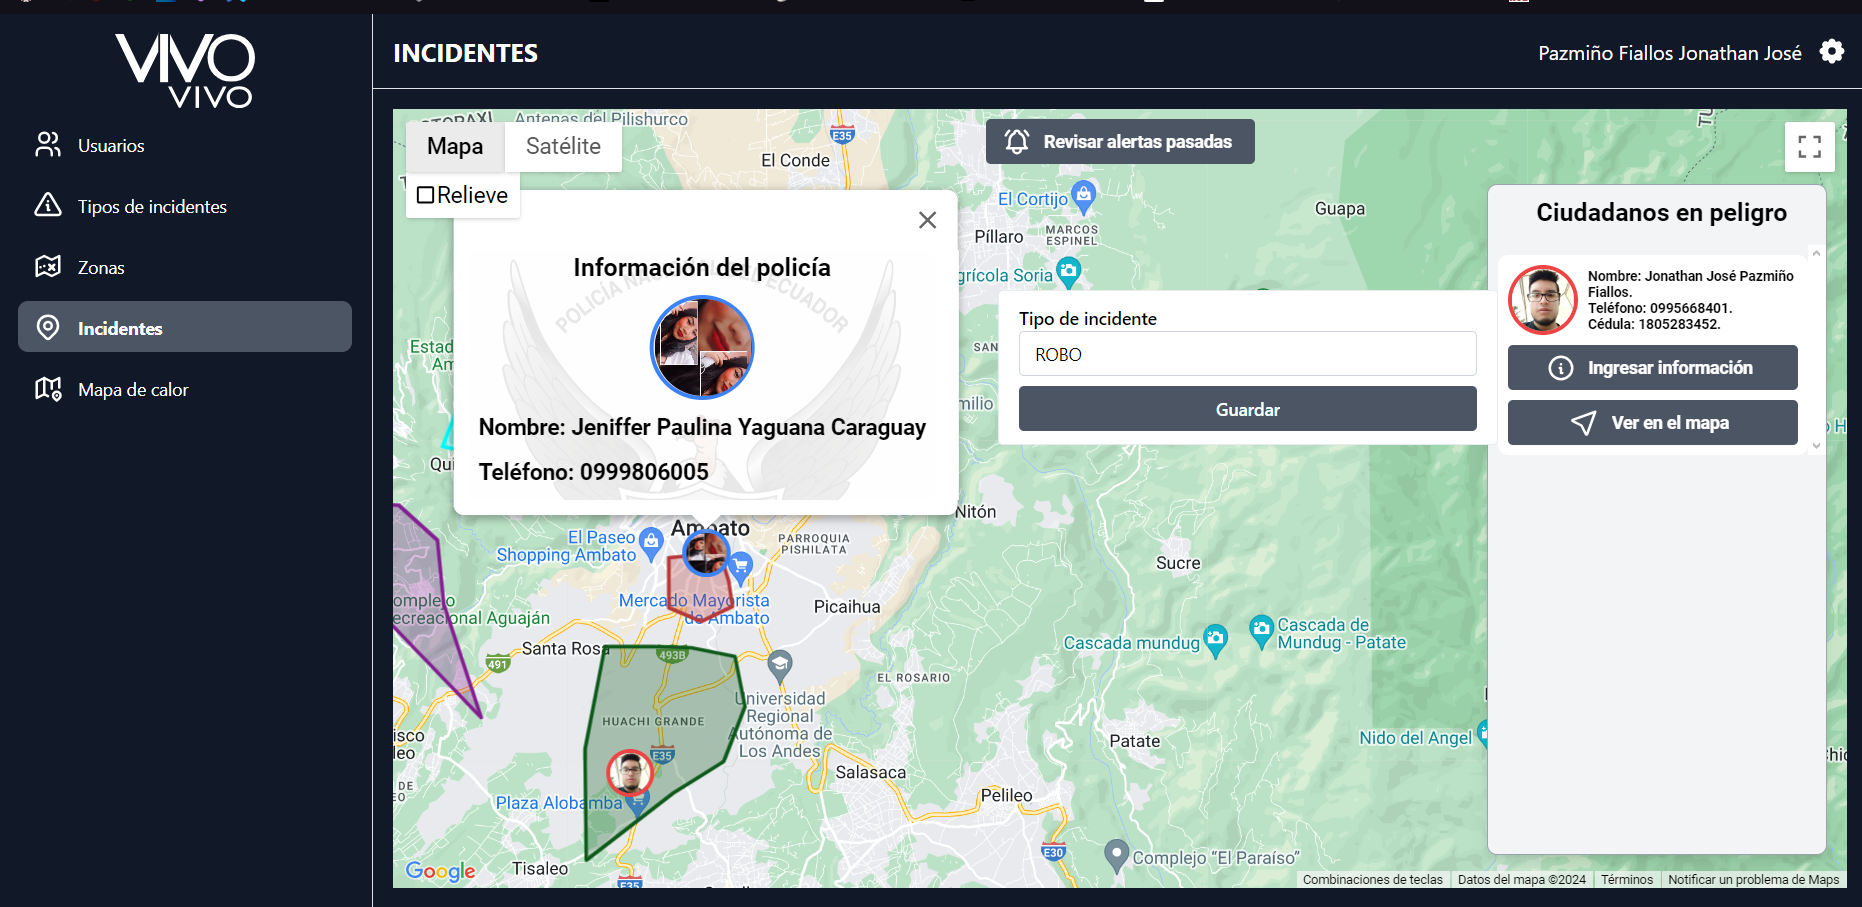
\includegraphics[width=0.8\textwidth]{chapters/III-resultados-y-discusion/resources/images/detalles-incidente-web.png}
    \caption{Detalles de incidente en el sistema web.}
    \label{fig:detalles-incidente-web}
\end{figure}

El usuario administrador podrá revisar las alertas de incidentes pasados mediante una tabla de entradas, en la cual se muestran los
campos de la información de los incidentes, como el tipo de incidente, la fecha y la ubicación, como se muestra en la Figura
\ref{fig:tabla-incidentes-web}.

\begin{figure}[H]
    \centering
    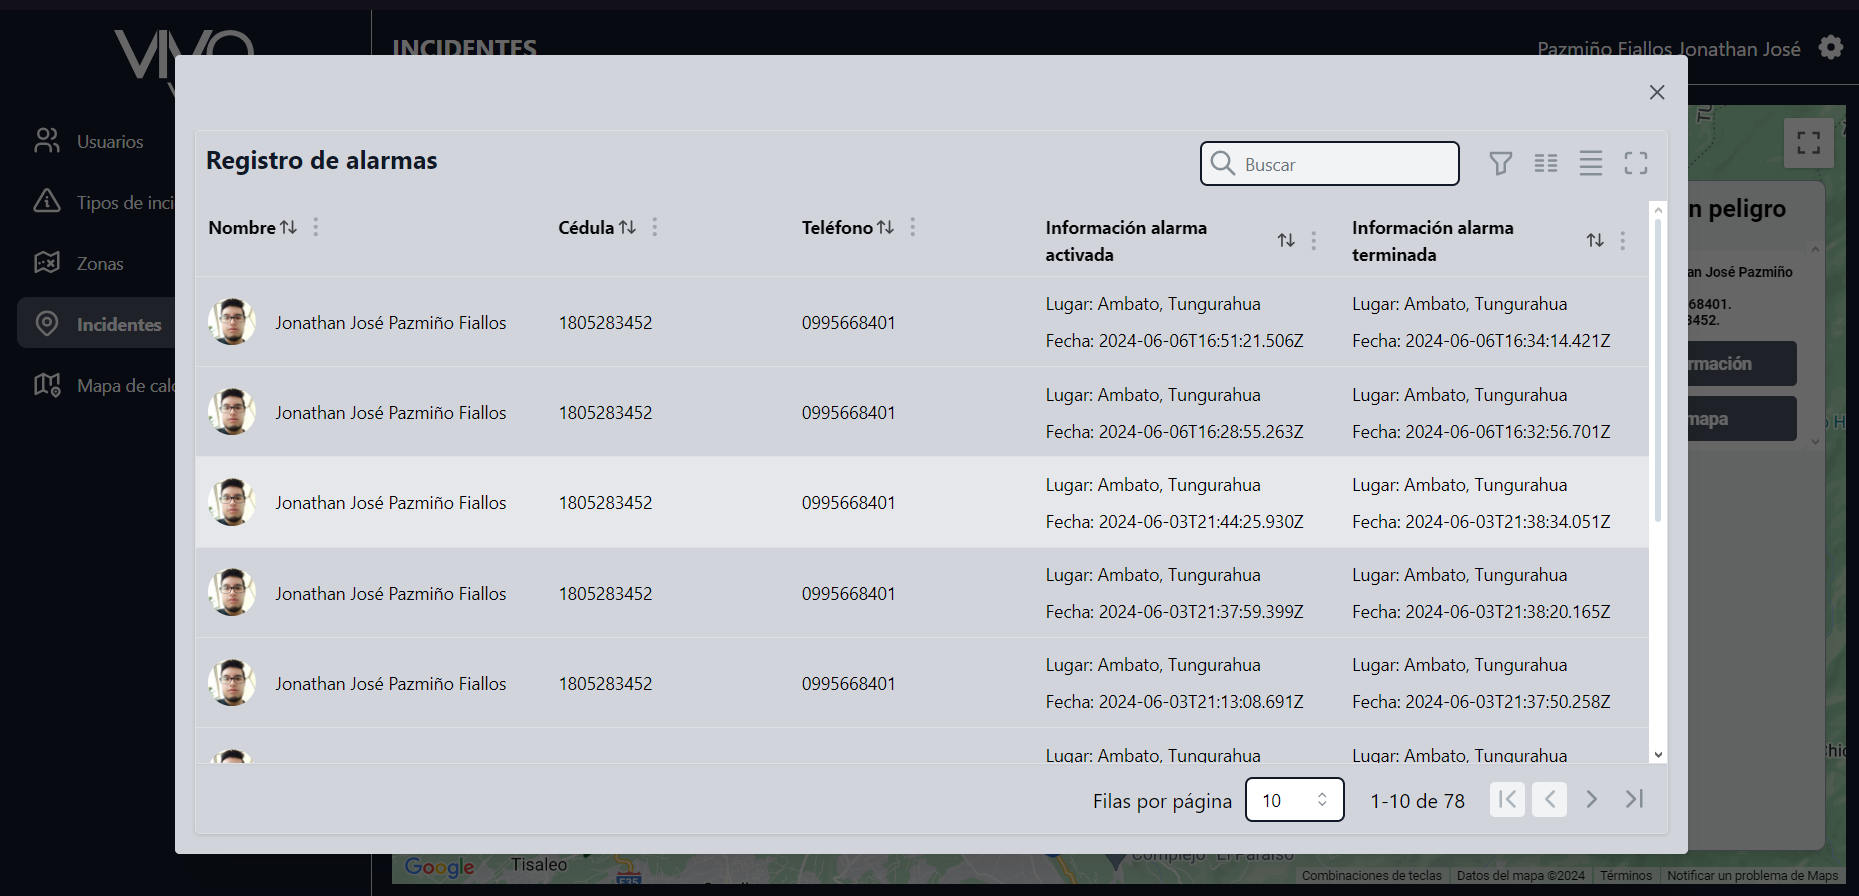
\includegraphics[width=0.8\textwidth]{chapters/III-resultados-y-discusion/resources/images/tabla-incidentes-web.png}
    \caption{Tabla de incidentes en el sistema web.}
    \label{fig:tabla-incidentes-web}
\end{figure}

\paragraph{Mapa de calor}
El mapa de calor en el sistema web permite al usuario administrador visualizar la densidad de incidentes reportados en un mapa
mediante un gradiente de colores, así como filtrar los incidentes por tipo y fecha, como se muestra en la Figura \ref{fig:mapa-de-calor-web}.

\begin{figure}[H]
    \centering
    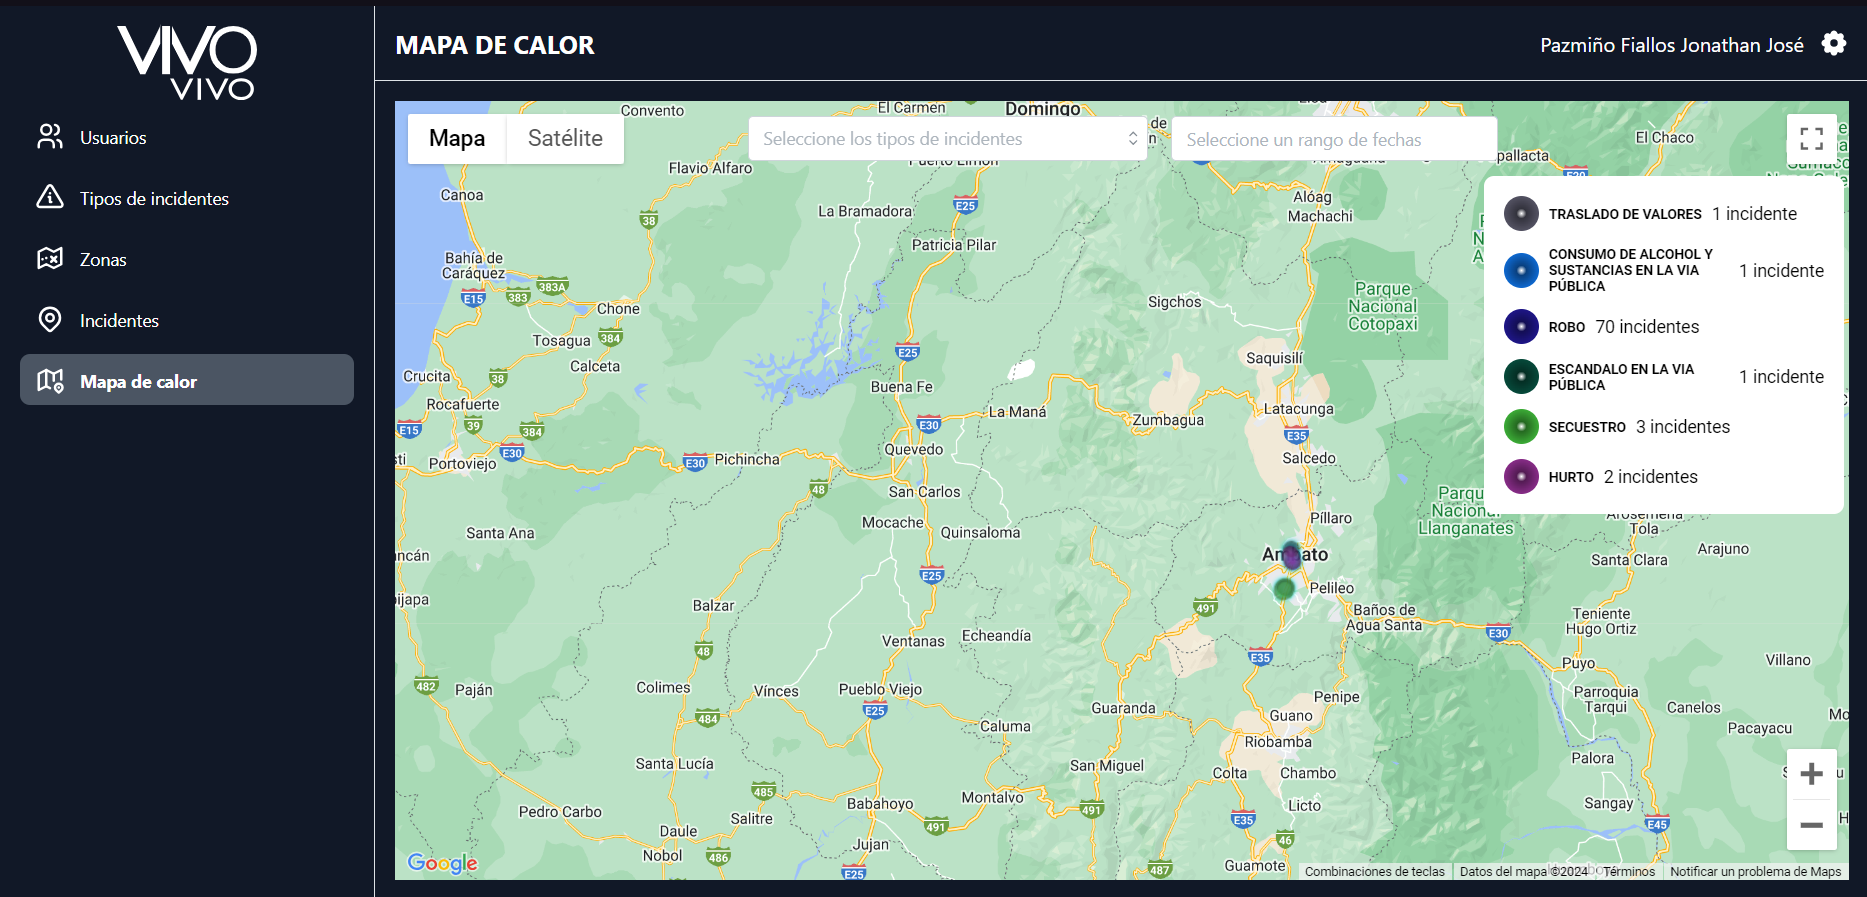
\includegraphics[width=0.8\textwidth]{chapters/III-resultados-y-discusion/resources/images/mapa-de-calor-web.png}
    \caption{Mapa de calor en el sistema web.}
    \label{fig:mapa-de-calor-web}
\end{figure}

\textbf{Aplicación móvil}
\bigbreak

\paragraph{Dependencias de la aplicación móvil}
Para crear el proyecto de Flutter se utilizó el comando "flutter create", el cual crea una aplicación de Flutter con
una estructura de carpetas y archivos predefinida. Las dependencias utilizadas en la aplicación móvil se gestionaron mediante flutter pub
y el archivo de configuración pubspec.yaml. En el Anexo \ref{apendix:dependencias-movil} se muestra las dependencias utilizadas en la
aplicación móvil.

\paragraph{Configuración de variables de entorno de la aplicación móvil}
Para la configuración de las variables de entorno de la aplicación móvil se utilizó un archivo .env, el cual contiene las propiedades de
de la aplicación, como la URL de la API, el api key de Google Maps, el api key de OneSignal y la URL para obtener las imágenes
de Cloudinary. En el Anexo \ref{apendix:configuracion-env-movil} se muestra el archivo .env con las variables de entorno de la aplicación móvil.

\paragraph{Configuración de la aplicación}
En Flutter, la configuración global de la aplicación se realiza mediante Providers y ChangeNotifier, los cuales permiten compartir datos y
funcionalidades entre los widgets. En el Anexo \ref{apendix:configuracion-aplicacion-movil} se muestra la configuración para los
proveedores de sesión, sockets, localización y gestión de datos en la aplicación móvil.

\paragraph{Inicio de sesión}
El inicio de sesión en la aplicación móvil se realiza mediante un formulario en el cual el usuario ingresa su correo electrónico y
contraseña, como se muestra en la Figura \ref{fig:inicio-sesion-movil}. Estas credenciales son enviadas a la API mediante una solicitud
POST para autenticar al usuario y obtener un token JWT, el cual se almacena en el almacenamiento local del dispositivo para mantener
la sesión activa, en el Anexo \ref{apendix:guardar-token-movil} se muestra el código para guardar el token en el almacenamiento local del
dispositivo.

\begin{figure}[H]
    \centering
    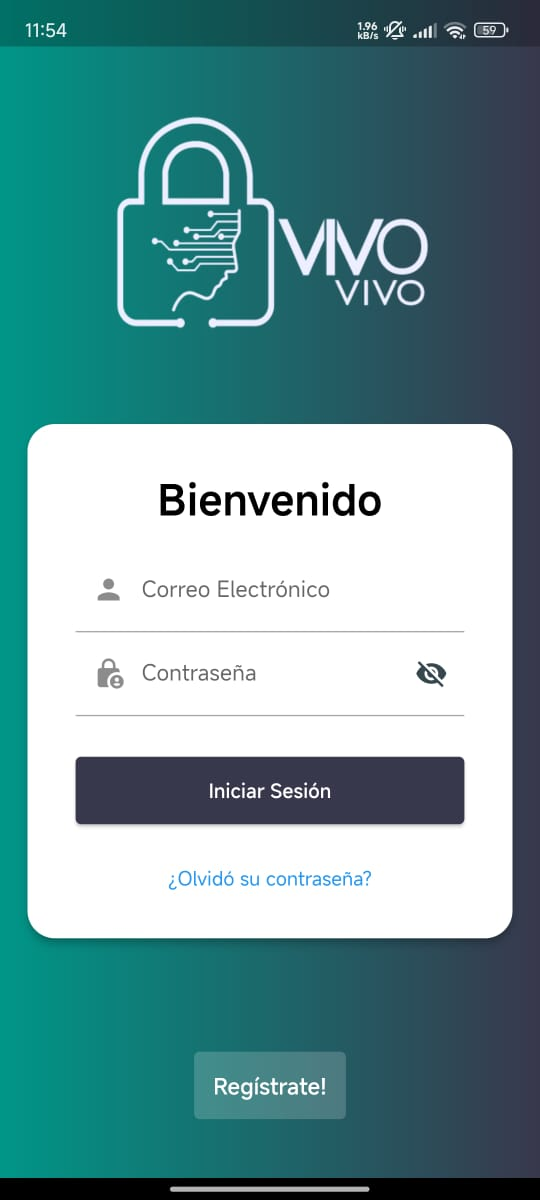
\includegraphics[width=0.3\textwidth]{chapters/III-resultados-y-discusion/resources/images/inicio-sesion-movil.png}
    \caption{Inicio de sesión en la aplicación móvil.}
    \label{fig:inicio-sesion-movil}
\end{figure}

\paragraph{Recuperar contraseña}
La recuperación de contraseña en la aplicación móvil se realiza mediante un formulario en el cual el usuario ingresa su correo electrónico,
como se muestra en la Figura \ref{fig:recuperar-contrasena-movil}. Una vez ingresado el correo electrónico, se envía una contraseña provisional
al correo electrónico del usuario con la cual podrá iniciar sesión y cambiar su contraseña, en la Figura \ref{fig:recuperar-contrasena-email}
se muestra el correo electrónico de recuperación de contraseña.

\begin{figure}[H]
    \centering
    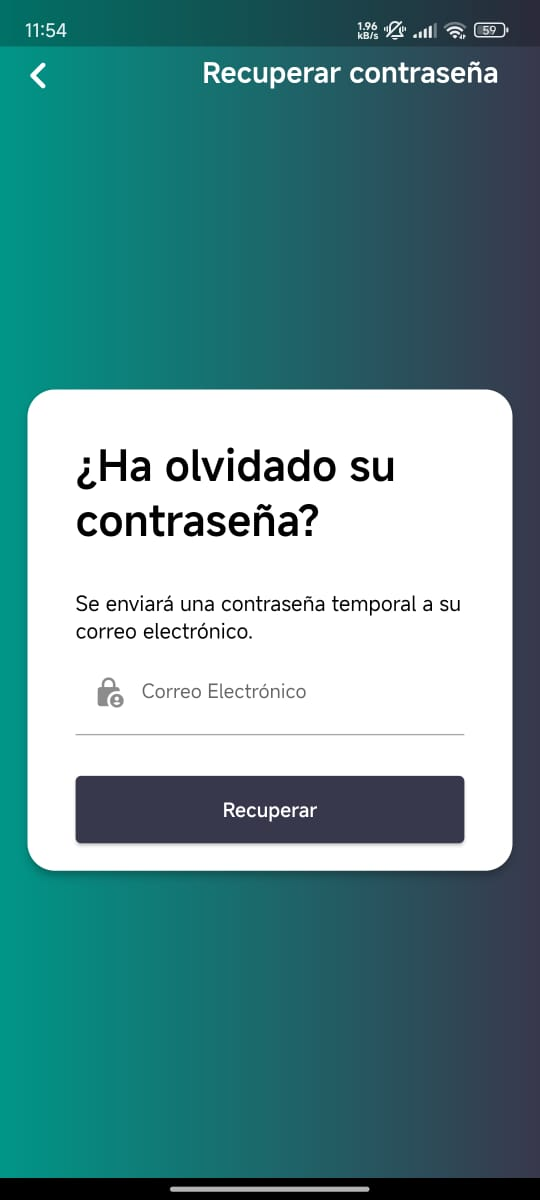
\includegraphics[width=0.3\textwidth]{chapters/III-resultados-y-discusion/resources/images/recuperar-contrasena-movil.png}
    \caption{Recuperar contraseña en la aplicación móvil.}
    \label{fig:recuperar-contrasena-movil}
\end{figure}

\begin{figure}[H]
    \centering
    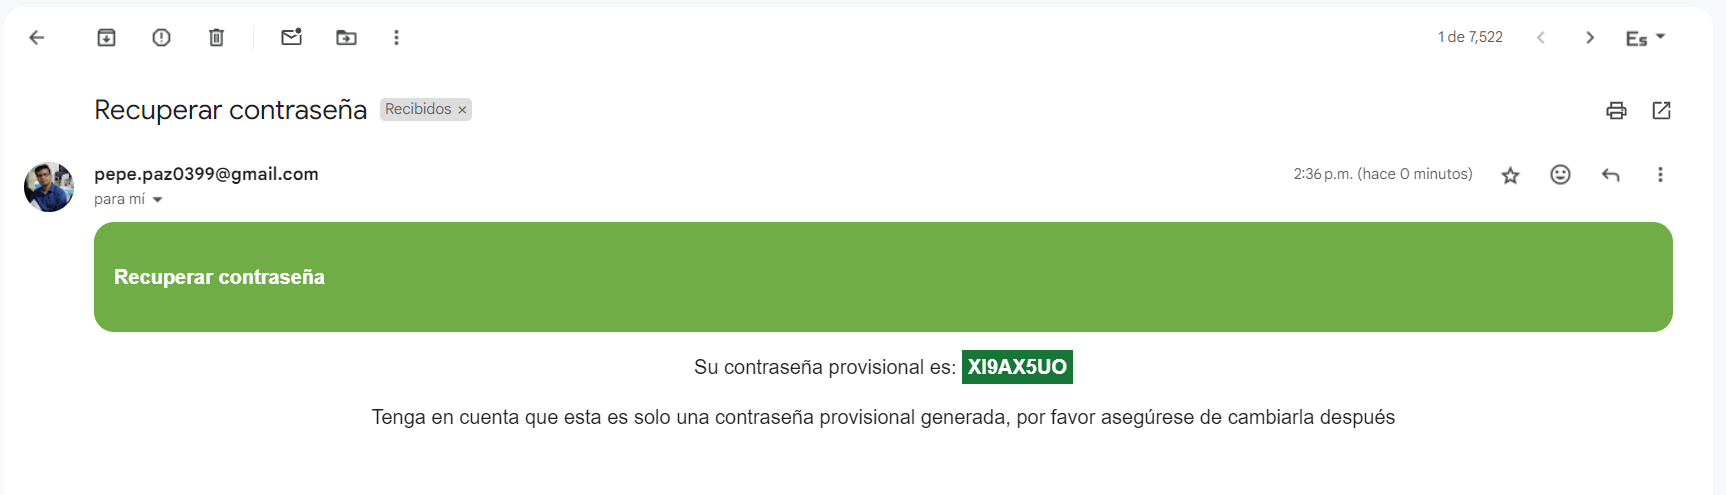
\includegraphics[width=1\textwidth]{chapters/III-resultados-y-discusion/resources/images/recuperar-contrasena-email.png}
    \caption{Correo electrónico de recuperación de contraseña.}
    \label{fig:recuperar-contrasena-email}
\end{figure}

\paragraph{Registro de usuario}
El registro de usuario en la aplicación móvil se realiza mediante un formulario en el cual el usuario ingresa su información personal,
como nombres, apellidos, correo electrónico, contraseña, género, etnia, entre otros, como se muestra en las Figuras \ref{fig:registro-usuario-movil-1}
y \ref{fig:registro-usuario-movil-2}. Para ingresar la dirección del usuario, se utilizó un campo de búsqueda de direcciones que permite
al usuario buscar su dirección en un mapa interactivo y seleccionarla, como se muestra en la Figura \ref{fig:registro-usuario-movil-3}.

\begin{figure}[H]
    \centering
    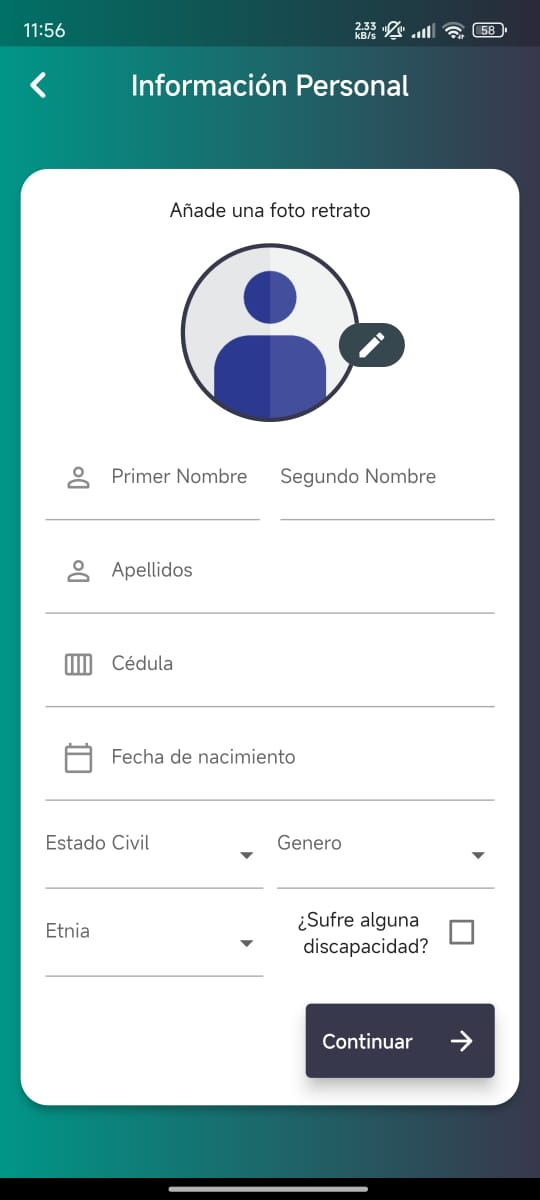
\includegraphics[width=0.3\textwidth]{chapters/III-resultados-y-discusion/resources/images/registro-usuario-movil-1.png}
    \caption{Registro de usuario en la aplicación móvil (Parte 1).}
    \label{fig:registro-usuario-movil-1}
\end{figure}

\begin{figure}[H]
    \centering
    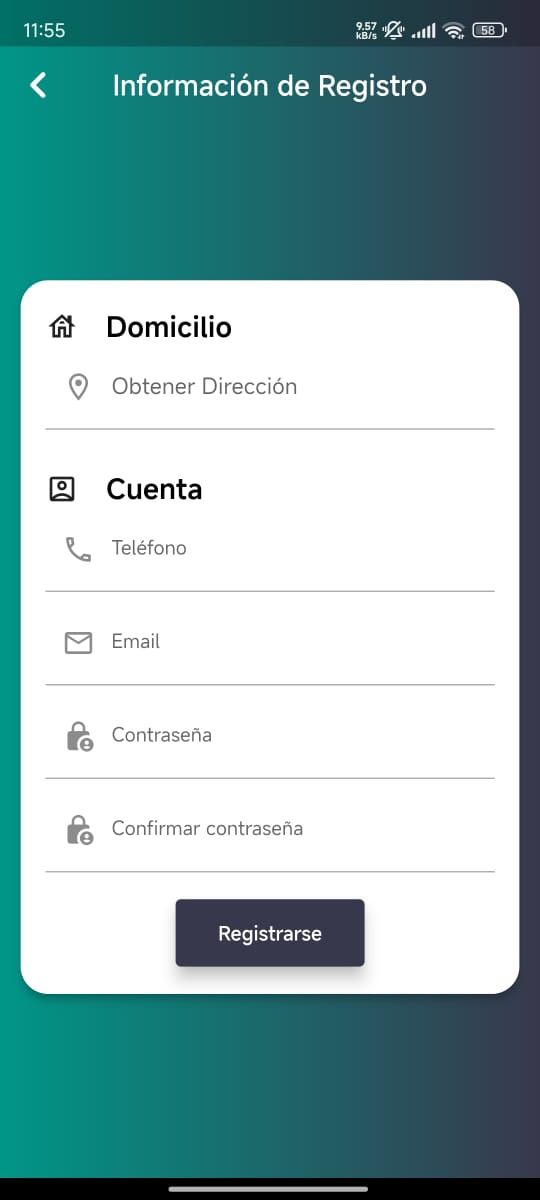
\includegraphics[width=0.3\textwidth]{chapters/III-resultados-y-discusion/resources/images/registro-usuario-movil-2.png}
    \caption{Registro de usuario en la aplicación móvil (Parte 2).}
    \label{fig:registro-usuario-movil-2}
\end{figure}

\begin{figure}[H]
    \centering
    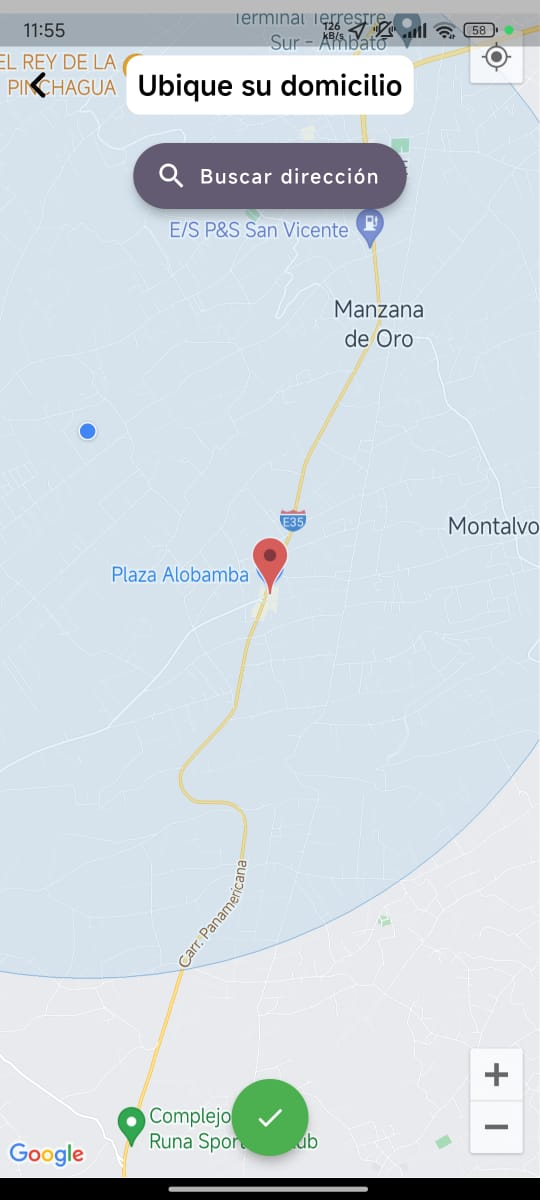
\includegraphics[width=0.3\textwidth]{chapters/III-resultados-y-discusion/resources/images/registro-usuario-movil-3.png}
    \caption{Registro de usuario en la aplicación móvil (Parte 3).}
    \label{fig:registro-usuario-movil-3}
\end{figure}

\paragraph{Pantalla principal}
La pantalla principal de la aplicación móvil muestra el botón de pánico en la parte central de la pantalla, el cual permite al usuario
enviar una alerta de emergencia a los miembros de su grupo familiar y a los policías en la zona de emergencia presionando el botón
durante 3 segundos, también el usuario puede seleccionar el tipo de incidente mediante un check, como se muestra en la Figura
\ref{fig:pantalla-principal-movil}.

\begin{figure}[H]
    \centering
    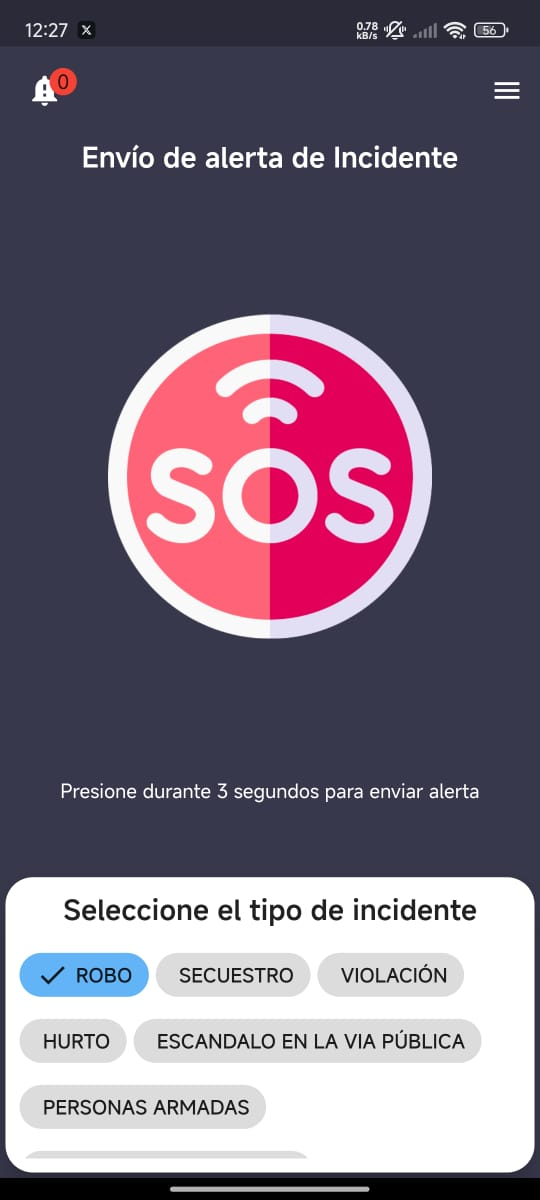
\includegraphics[width=0.3\textwidth]{chapters/III-resultados-y-discusion/resources/images/pantalla-principal-movil.png}
    \caption{Pantalla principal de la aplicación móvil.}
    \label{fig:pantalla-principal-movil}
\end{figure}

\paragraph{Menú de usuario}
El menú de usuario en la aplicación móvil permite al usuario acceder a las opciones tales como cambiar contraseña, cerrar sesión y
gestionar el grupo familiar, como se muestra en la Figura \ref{fig:menu-usuario-movil}.

\begin{figure}[H]
    \centering
    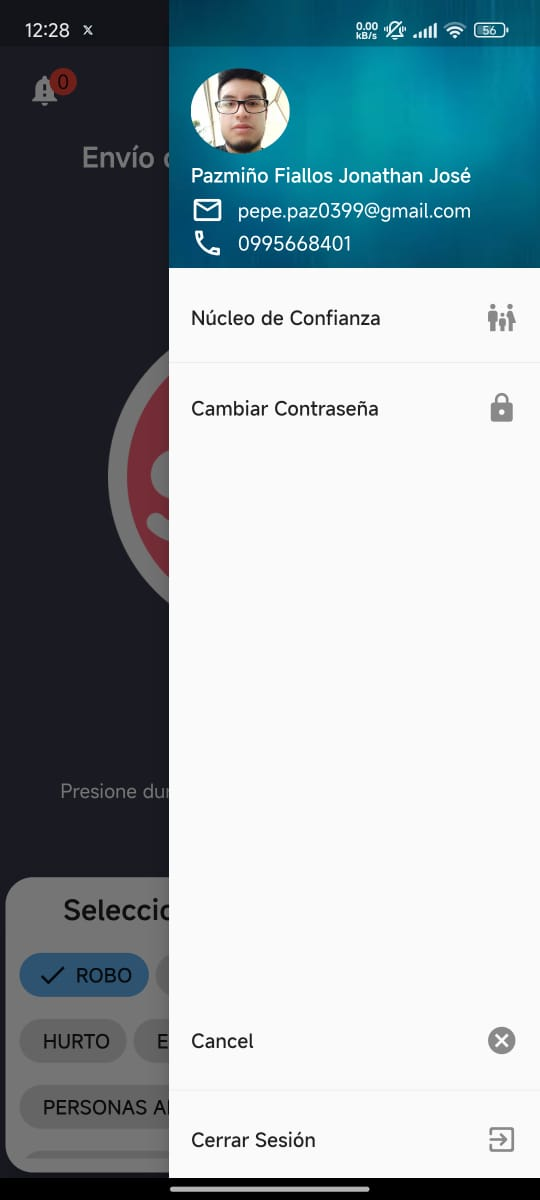
\includegraphics[width=0.3\textwidth]{chapters/III-resultados-y-discusion/resources/images/menu-usuario-movil.png}
    \caption{Menú de usuario en la aplicación móvil.}
    \label{fig:menu-usuario-movil}
\end{figure}

\paragraph{Gestión de grupo familiar}
La gestión del grupo familiar en la aplicación móvil se realiza mediante una lista en la cual el usuario podrá visualizar a
los miembros de su grupo familiar, como se muestra en la Figura \ref{fig:grupo-familiar-movil}. El usuario podrá agregar
miembros a su grupo familiar mediante un formulario en el cual ingresará la cédula de identidad del usuario que desee
agregar, como se muestra en la Figura \ref{fig:agregar-miembro-movil}.

\begin{figure}[H]
    \centering
    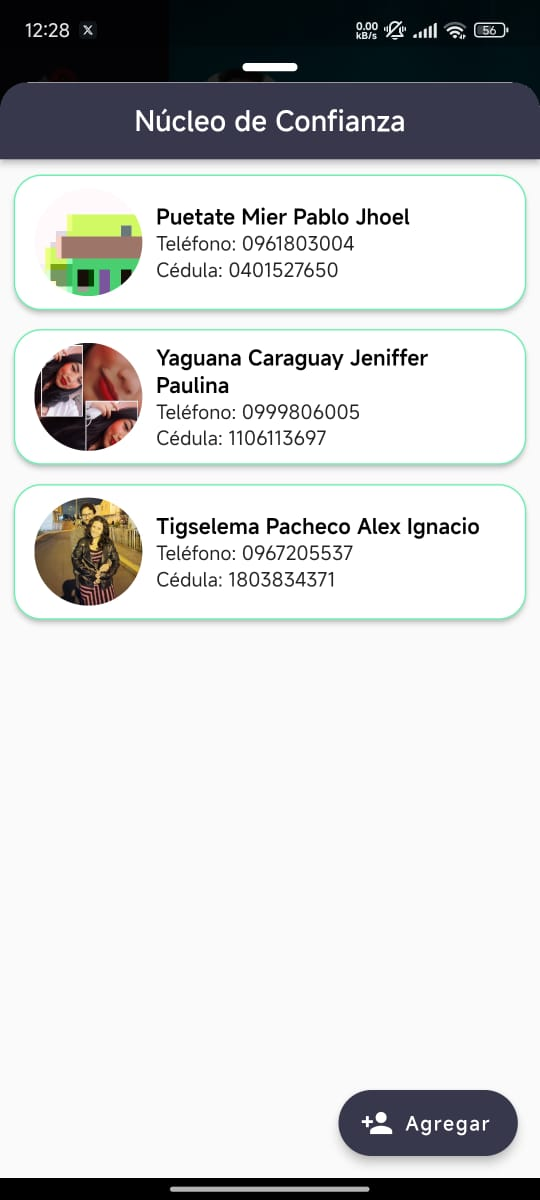
\includegraphics[width=0.3\textwidth]{chapters/III-resultados-y-discusion/resources/images/grupo-familiar-movil.png}
    \caption{Gestión de grupo familiar en la aplicación móvil.}
    \label{fig:grupo-familiar-movil}
\end{figure}

\begin{figure}[H]
    \centering
    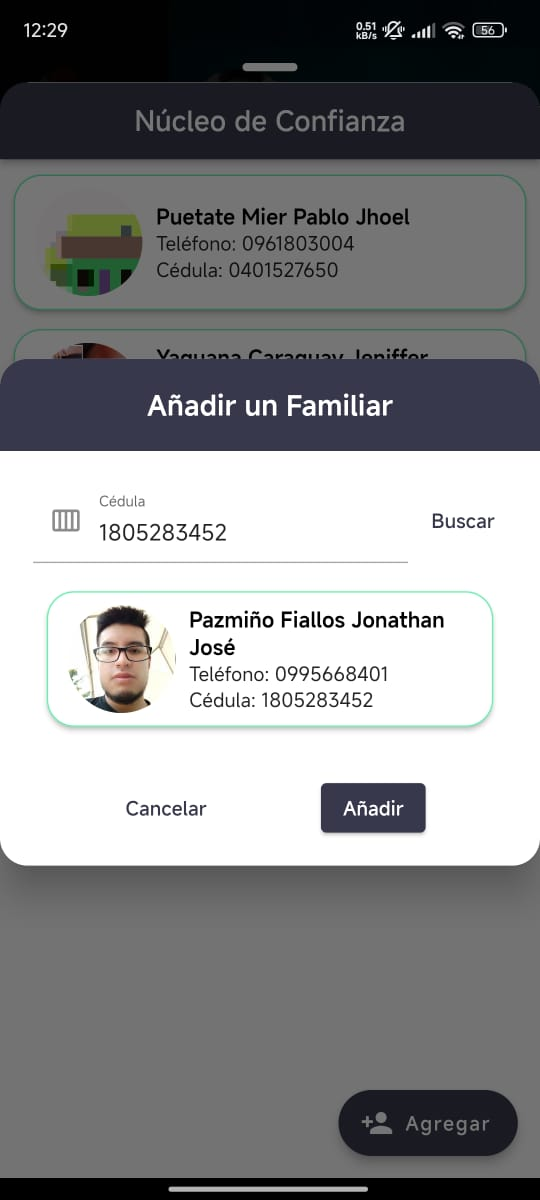
\includegraphics[width=0.3\textwidth]{chapters/III-resultados-y-discusion/resources/images/agregar-miembro-movil.png}
    \caption{Agregar miembro al grupo familiar en la aplicación móvil.}
    \label{fig:agregar-miembro-movil}
\end{figure}

\paragraph{Cambiar contraseña}
La opción de cambiar contraseña en la aplicación móvil permite al usuario modificar su contraseña ingresando la contraseña actual,
la nueva contraseña y la confirmación de la nueva contraseña, como se muestra en la Figura \ref{fig:cambiar-contrasena-movil}.

\begin{figure}[H]
    \centering
    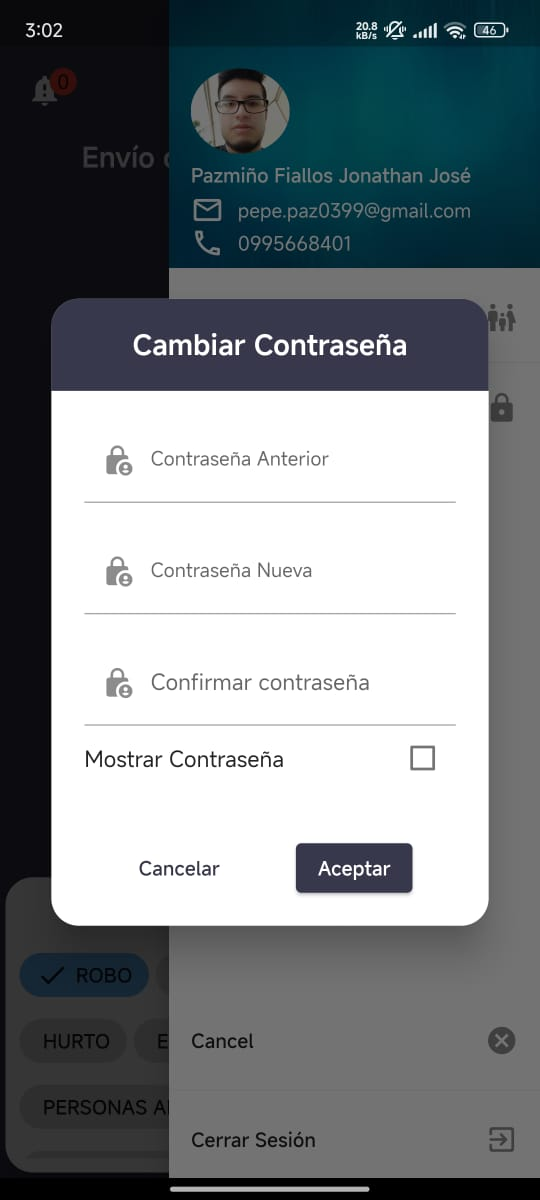
\includegraphics[width=0.3\textwidth]{chapters/III-resultados-y-discusion/resources/images/cambiar-contrasena-movil.png}
    \caption{Cambiar contraseña en la aplicación móvil.}
    \label{fig:cambiar-contrasena-movil}
\end{figure}

\paragraph{Alertas recibidas}
Las alertas recibidas en la aplicación móvil se visualizan mediante una lista en la cual se muestra el estado de cada miembro del
grupo familiar. Cuando un miembro del grupo familiar envía una alerta de emergencia, se muestra una notificación en el dispositivo
del usuario, como se puede observar en la Figura \ref{fig:notificacion-recibida-movil} y el estado del miembro cambia a "En peligro", como se
puede observar en la Figura \ref{fig:alerta-recibida-movil}. El usuario podrá visualizar la ubicación en tiempo real del miembro en
peligro seleccionando el botón "Seguir ubicación", lo cual mostrará la en un mapa la ubicación del miembro en peligro y la ubicación
del usuario, como se muestra en la Figura \ref{fig:seguir-ubicacion-movil}.

\begin{figure}[H]
    \centering
    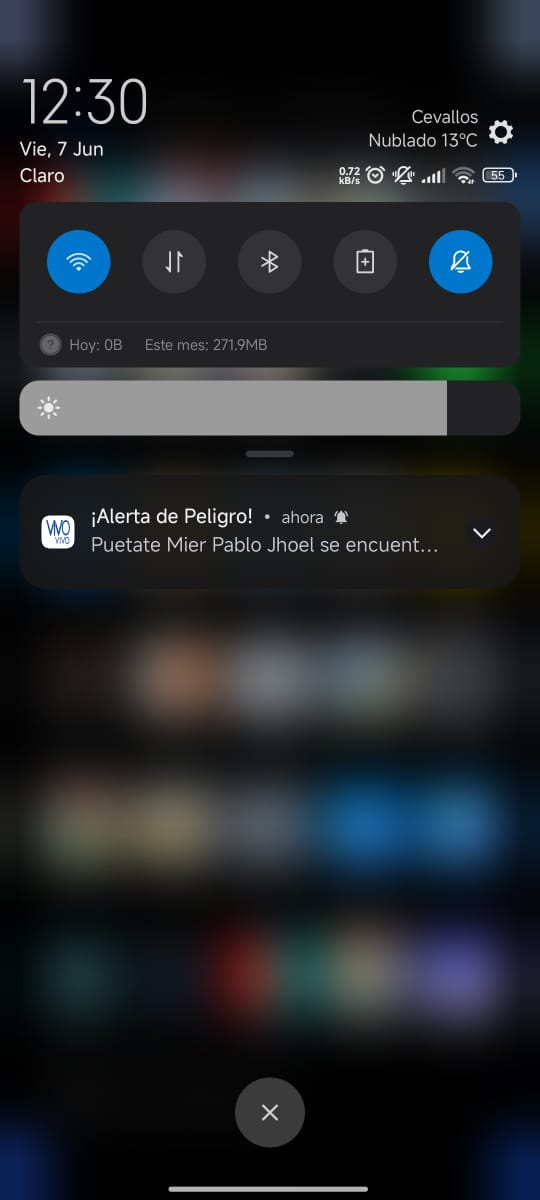
\includegraphics[width=0.3\textwidth]{chapters/III-resultados-y-discusion/resources/images/notificacion-recibida-movil.png}
    \caption{Notificación de alerta recibida en la aplicación móvil.}
    \label{fig:notificacion-recibida-movil}
\end{figure}

\begin{figure}[H]
    \centering
    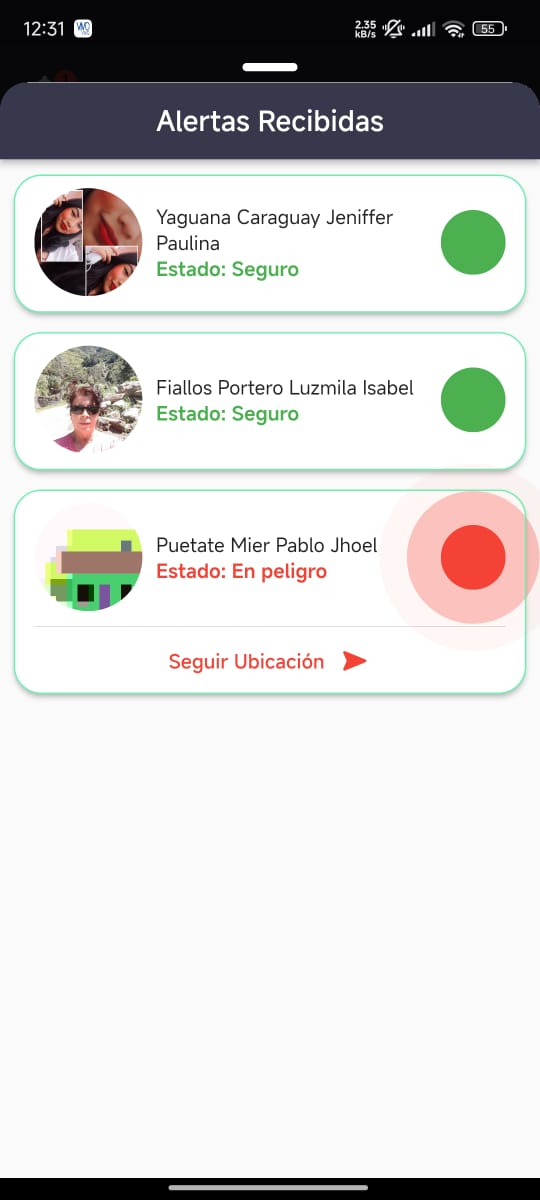
\includegraphics[width=0.3\textwidth]{chapters/III-resultados-y-discusion/resources/images/alerta-recibida-movil.png}
    \caption{Alerta recibida en la aplicación móvil.}
    \label{fig:alerta-recibida-movil}
\end{figure}

\begin{figure}[H]
    \centering
    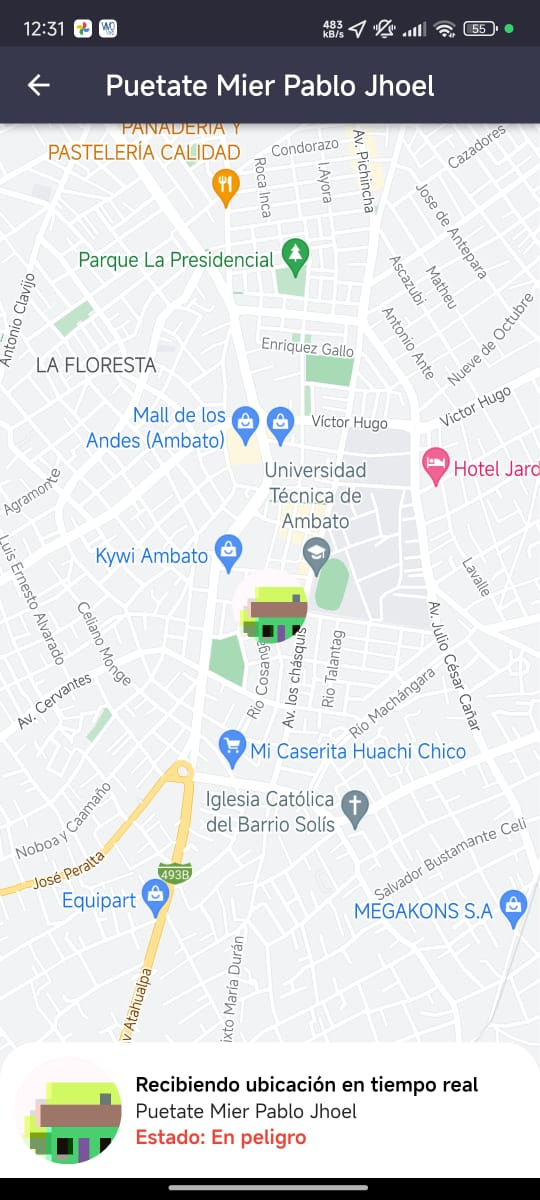
\includegraphics[width=0.3\textwidth]{chapters/III-resultados-y-discusion/resources/images/seguir-ubicacion-movil.png}
    \caption{Seguir ubicación en la aplicación móvil.}
    \label{fig:seguir-ubicacion-movil}
\end{figure}

\textbf{Modelo analítico de BI}
\bigbreak

Para el diseño del modelo analítico de BI se utilizó la metodología Hefesto, ya que esta facilita la construcción de un
Data Warehouse y aporta información útil para mejorar el rendimiento \cite{darioDATAWAREHOUSINGMarco2018}.

% \paragraph{Carta de diseño para el modelo dimensional}

La carta de diseño para el modelo dimensional se utiliza para describir el proceso de diseño de un modelo dimensional
siguiendo los pasos de la metodología Hefesto. Estos pasos incluyen la selección del proceso de negocio, la declaración
del grano, la identificación de las dimensiones y sus atributos, la identificación de las tablas de hechos y sus métricas,
y el diseño del esquema dimensional. A continuación, se presenta cada uno de estos pasos.

\begin{itemize}
    \item Seleccionar el proceso de negocio:
          \begin{itemize}
              \item Identificar las pregustas del negocio.
              \item Identificar indicadores y perspectivas.
              \item Diseñar el modelo conceptual.
          \end{itemize}
    \item Declarar el grano.
    \item Identificar las dimensiones y sus atributos.
    \item Identificar las tablas de hechos y sus métricas.
    \item Diseñar el esquema dimensional
\end{itemize}

\paragraph{Seleccionar el proceso de negocio}

\paragraph{Preguntas del negocio}

El objetivo principal del sistema de reportería de incidentes delictivos es recolectar y analizar información
sobre los incidentes delictivos reportados a través de un sistema de alarma, así como detalles de los usuarios
y datos geográficos relevantes para apoyar la toma de decisiones de las autoridades policiales.

\paragraph{Identificar indicadores y perspectivas}

\begin{itemize}
    \item Determinar el número de incidentes por tipo de incidente y zona de vigilancia.
    \item Analizar la distribución de incidentes por género, discapacidad, etnia y edad de los usuarios.
    \item Identificar las zonas con mayor número de incidentes para optimizar la vigilancia policial.
\end{itemize}

\begin{longtable}{|p{5cm}|p{5cm}|}
    \caption{Indicadores y perspectivas en base las pregustas de negocio} \label{tab:indicadores-perspectivas} \\

    \hline \multicolumn{1}{|c|}{\textbf{Indicadores}} & \multicolumn{1}{|c|}{\textbf{Perspectivas}}            \\ \hline
    \endfirsthead

    \multicolumn{2}{c}%
    {{\normalfont \tablename\ \thetable{} -- continuación de la página anterior}}                              \\
    \hline \multicolumn{1}{|c|}{\textbf{Indicadores}} & \multicolumn{1}{|c|}{\textbf{Perspectivas}}            \\ \hline
    \endhead

    \hline \multicolumn{2}{|r|}{{Continua en la siguiente página}}                                             \\ \hline
    \endfoot

    \hline \hline
    \endlastfoot
    Número de incidentes                              & Tipo de Alarma                                         \\\hline
    Número de incidentes                              & Tipo de Incidente                                      \\\hline
    Número de incidentes                              & Zona de Vigilancia                                     \\\hline
    Número de incidentes                              & Género, Discapacidad, Etnia, Estado Civil              \\
\end{longtable}

En base a los indicadores y perspectivas identificados, se estableció como KPI principal el número de incidentes
delictivos reportados, ya que este indicador permite medir la frecuencia de los delitos reportados en una determinada
área o periodo de tiempo.

\paragraph{Declarar el grano}

El grano del modelo dimensional es un único incidente delictivo reportado. Esto implica que cada registro en la
tabla de hechos representa un incidente específico.

\paragraph{Identificar las dimensiones y sus atributos}

En las Tablas \ref{tab:dimension-tiempo}, \ref{tab:dimension-usuarios}, \ref{tab:dimension-tipo-de-alarma},
\ref{tab:dimension-tipo-de-incidente} y \ref{tab:dimension-zona-de-vigilancia} se presentan las dimensiones y
sus atributos identificados para el modelo dimensional.

\begin{longtable}{|p{6cm}|p{6cm}|}
    \caption{Dimensión de tiempo con sus atributos} \label{tab:dimension-tiempo}             \\

    \hline \multicolumn{1}{|c|}{\textbf{Campo}} & \multicolumn{1}{|c|}{\textbf{Descripción}} \\ \hline
    \endfirsthead

    \multicolumn{2}{c}%
    {{\normalfont \tablename\ \thetable{} -- continuación de la página anterior}}            \\
    \hline \multicolumn{1}{|c|}{\textbf{Campo}} & \multicolumn{1}{|c|}{\textbf{Descripción}} \\ \hline
    \endhead

    \hline \multicolumn{2}{|r|}{{Continua en la siguiente página}}                           \\ \hline
    \endfoot

    \hline \hline
    \endlastfoot
    fechaID                                     & Identificador único para cada fecha        \\\hline
    fecha                                       & Fecha completa del incidente (YYYY-MM-DD)  \\\hline
    anio                                        & Año en que ocurrió el incidente            \\\hline
    mes                                         & Mes en que ocurrió el incidente            \\\hline
    día                                         & Día en que ocurrió el incidente            \\\hline
    trimestre                                   & Trimestre en que ocurrió el incidente      \\\hline
    semestre                                    & Semestre en que ocurrió el incidente       \\\hline
    hora                                        & Hora en que ocurrió el incidente           \\
\end{longtable}

\begin{longtable}{|p{6cm}|p{6cm}|}
    \caption{Dimensión de usuarios con sus atributos} \label{tab:dimension-usuarios}         \\

    \hline \multicolumn{1}{|c|}{\textbf{Campo}} & \multicolumn{1}{|c|}{\textbf{Descripción}} \\ \hline
    \endfirsthead

    \multicolumn{2}{c}%
    {{\normalfont \tablename\ \thetable{} -- continuación de la página anterior}}            \\
    \hline \multicolumn{1}{|c|}{\textbf{Campo}} & \multicolumn{1}{|c|}{\textbf{Descripción}} \\ \hline
    \endhead

    \hline \multicolumn{2}{|r|}{{Continua en la siguiente página}}                           \\ \hline
    \endfoot

    \hline \hline
    \endlastfoot
    usuarioID                                   & Identificador único del usuario            \\\hline
    género                                      & Género del usuario                         \\\hline
    discapacidad                                & Estado de discapacidad del usuario         \\\hline
    etnia                                       & Etnia del usuario                          \\\hline
    estadoCivil                                 & Estado civil del usuario                   \\\hline
    edad                                        & Edad del usuario                           \\
\end{longtable}

\begin{longtable}{|p{6cm}|p{6cm}|}
    \caption{Dimensión de tipo de alarma con sus atributos} \label{tab:dimension-tipo-de-alarma} \\

    \hline \multicolumn{1}{|c|}{\textbf{Campo}} & \multicolumn{1}{|c|}{\textbf{Descripción}}     \\ \hline
    \endfirsthead

    \multicolumn{2}{c}%
    {{\normalfont \tablename\ \thetable{} -- continuación de la página anterior}}                \\
    \hline \multicolumn{1}{|c|}{\textbf{Campo}} & \multicolumn{1}{|c|}{\textbf{Descripción}}     \\ \hline
    \endhead

    \hline \multicolumn{2}{|r|}{{Continua en la siguiente página}}                               \\ \hline
    \endfoot

    \hline \hline
    \endlastfoot
    tipoAlarmaID                                & Identificador único del tipo de alarma         \\\hline
    nombreTipoAlarma                            & Nombre del tipo de alarma                      \\
\end{longtable}

\begin{longtable}{|p{6cm}|p{6cm}|}
    \caption{Dimensión de tipo de incidente con sus atributos} \label{tab:dimension-tipo-de-incidente} \\

    \hline \multicolumn{1}{|c|}{\textbf{Campo}} & \multicolumn{1}{|c|}{\textbf{Descripción}}           \\ \hline
    \endfirsthead

    \multicolumn{2}{c}%
    {{\normalfont \tablename\ \thetable{} -- continuación de la página anterior}}                      \\
    \hline \multicolumn{1}{|c|}{\textbf{Campo}} & \multicolumn{1}{|c|}{\textbf{Descripción}}           \\ \hline
    \endhead

    \hline \multicolumn{2}{|r|}{{Continua en la siguiente página}}                                     \\ \hline
    \endfoot

    \hline \hline
    \endlastfoot
    tipoIncidenteID                             & Identificador único del tipo de incidente            \\\hline
    nombreTipoIncidente                         & Nombre del tipo de incidente                         \\
\end{longtable}

\begin{longtable}{|p{6cm}|p{6cm}|}
    \caption{Dimensión de zonas de vigilancia con sus atributos} \label{tab:dimension-zonas-vigilancia} \\

    \hline \multicolumn{1}{|c|}{\textbf{Campo}} & \multicolumn{1}{|c|}{\textbf{Descripción}}            \\ \hline
    \endfirsthead

    \multicolumn{2}{c}%
    {{\normalfont \tablename\ \thetable{} -- continuación de la página anterior}}                       \\
    \hline \multicolumn{1}{|c|}{\textbf{Campo}} & \multicolumn{1}{|c|}{\textbf{Descripción}}            \\ \hline
    \endhead

    \hline \multicolumn{2}{|r|}{{Continua en la siguiente página}}                                      \\ \hline
    \endfoot

    \hline \hline
    \endlastfoot
    zonaVigilanciaID                            & Identificador único de la zona de vigilancia          \\\hline
    polígono                                    & Representación geográfica de la zona de vigilancia    \\\hline
    nombreZonaVigilancia                        & Nombre de la zona de vigilancia                       \\
\end{longtable}

\begin{longtable}{|p{6cm}|p{6cm}|}
    \caption{Dimensión de ubicación con sus atributos} \label{tab:dimension-zonas-vigilancia} \\

    \hline \multicolumn{1}{|c|}{\textbf{Campo}} & \multicolumn{1}{|c|}{\textbf{Descripción}}  \\ \hline
    \endfirsthead

    \multicolumn{2}{c}%
    {{\normalfont \tablename\ \thetable{} -- continuación de la página anterior}}             \\
    \hline \multicolumn{1}{|c|}{\textbf{Campo}} & \multicolumn{1}{|c|}{\textbf{Descripción}}  \\ \hline
    \endhead

    \hline \multicolumn{2}{|r|}{{Continua en la siguiente página}}                            \\ \hline
    \endfoot

    \hline \hline
    \endlastfoot
    ubicacionID                                 & Identificador único de la ubicación         \\\hline
    canton                                      & Cantón del lugar del incidente              \\\hline
    ciudad                                      & Ciudad del lugar del incidente              \\
\end{longtable}

\paragraph{Identificar las tablas de hechos y sus métricas}

En la Tabla \ref{tab:hechos-incidentes-delictivos} se presentan los hechos de incidentes delictivos y sus atributos.

\begin{longtable}{|p{6cm}|p{6cm}|}
    \caption{Hechos de incidentes delictivos con sus atributos} \label{tab:hechos-incidentes-delictivos}     \\

    \hline \multicolumn{1}{|c|}{\textbf{Campo}} & \multicolumn{1}{|c|}{\textbf{Descripción}}                 \\ \hline
    \endfirsthead

    \multicolumn{2}{c}%
    {{\normalfont \tablename\ \thetable{} -- continuación de la página anterior}}                            \\
    \hline \multicolumn{1}{|c|}{\textbf{Campo}} & \multicolumn{1}{|c|}{\textbf{Descripción}}                 \\ \hline
    \endhead

    \hline \multicolumn{2}{|r|}{{Continua en la siguiente página}}                                           \\ \hline
    \endfoot

    \hline \hline
    \endlastfoot
    incidenteID                                 & Clave primaria de la tabla de hechos incidentes delictivos \\\hline
    fechaID                                     & Clave foránea a la dimensión de tiempo                     \\\hline
    usuarioID                                   & Clave foránea a la dimensión de usuarios                   \\\hline
    tipoAlarmaID                                & Clave foránea a la dimensión de tipo de alarma             \\\hline
    tipoIncidenteID                             & Clave foránea a la dimensión de tipo de incidente          \\\hline
    zonaVigilanciaID                            & Clave foránea a la dimensión de zonas de vigilancia        \\\hline
    ubicacionID                                 & Clave foránea a la dimensión de ubicación geográfica       \\\hline
    numeroIncidentes                            & Número de incidentes reportados                            \\\hline
\end{longtable}

\paragraph{Esquema dimensional}

En la Figura \ref{fig:esquema-modelo-dimensional} se muestra el esquema del modelo dimensional propuesto para el sistema de reportería de incidentes delictivos.

\begin{figure}[H]
    \centering
    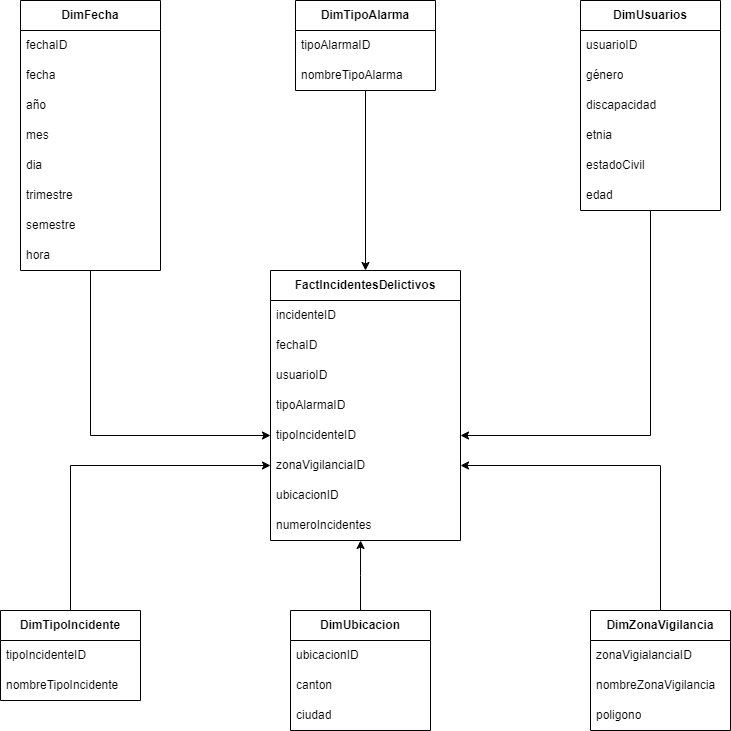
\includegraphics[width=1\textwidth]{chapters/III-resultados-y-discusion/resources/images/esquema-modelo-dimensional.png}
    \caption{Esquema del modelo dimensional para el sistema de reportería de incidentes delictivos}
    \label{fig:esquema-modelo-dimensional}
\end{figure}

\paragraph{Proceso ETL}

Una vez definido el modelo dimensional, se procedió a diseñar el proceso de extracción, transformación y carga (ETL) de los datos.
Para ello, se utilizó la herramienta de ETL de visual studio, la cual permite extraer datos de diferentes fuentes, transformarlos
y cargarlos en el modelo dimensional. En la Figura \ref{fig:etl-bi} se muestra el diseño del proceso ETL para el modelo dimensional.

\begin{figure}[H]
    \centering
    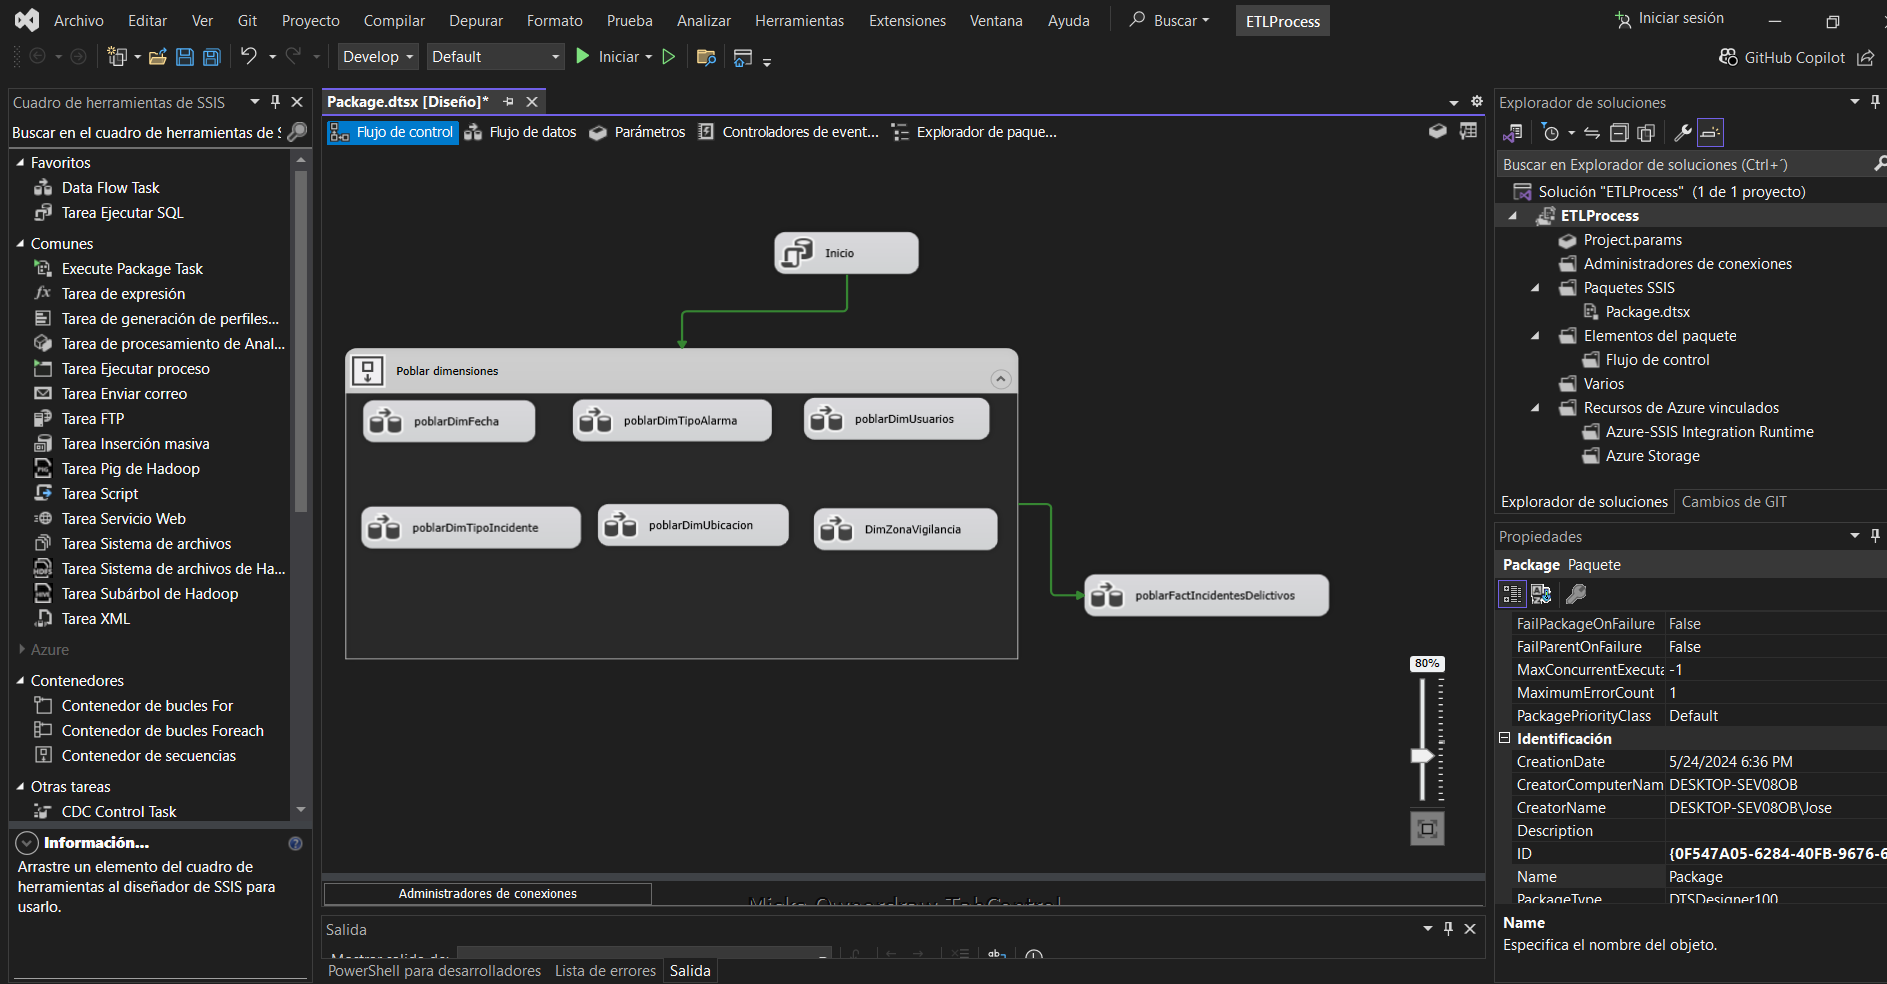
\includegraphics[width=0.8\textwidth]{chapters/III-resultados-y-discusion/resources/images/etl-bi.png}
    \caption{Diseño del proceso ETL para el modelo dimensional.}
    \label{fig:etl-bi}
\end{figure}

El proceso ETL inicia con la limpieza de las tablas que componen el modelo dimensional. Esto se realiza mediante la ejecución de un
script SQL que elimina los registros de las tablas de hechos y dimensiones, como se puede observar en la Figura\ref{fig:limpieza-bi}.
Una vez limpias las tablas, se procede a extraer los datos de las fuentes de datos. En este caso, se utilizó un origen de datos de
ADO.NET para extraer los datos desde PostgreSQL. Además, se utilizó el componente de Data Conversion para convertir los datos a un
formato compatible con el destino en una base de datos de SQL Server. Finalmente, se cargan los datos mediante el componente de OLE
DB Destination, como se puede observar en la Figura \ref{fig:extraccion-bi}.

\begin{figure}[H]
    \centering
    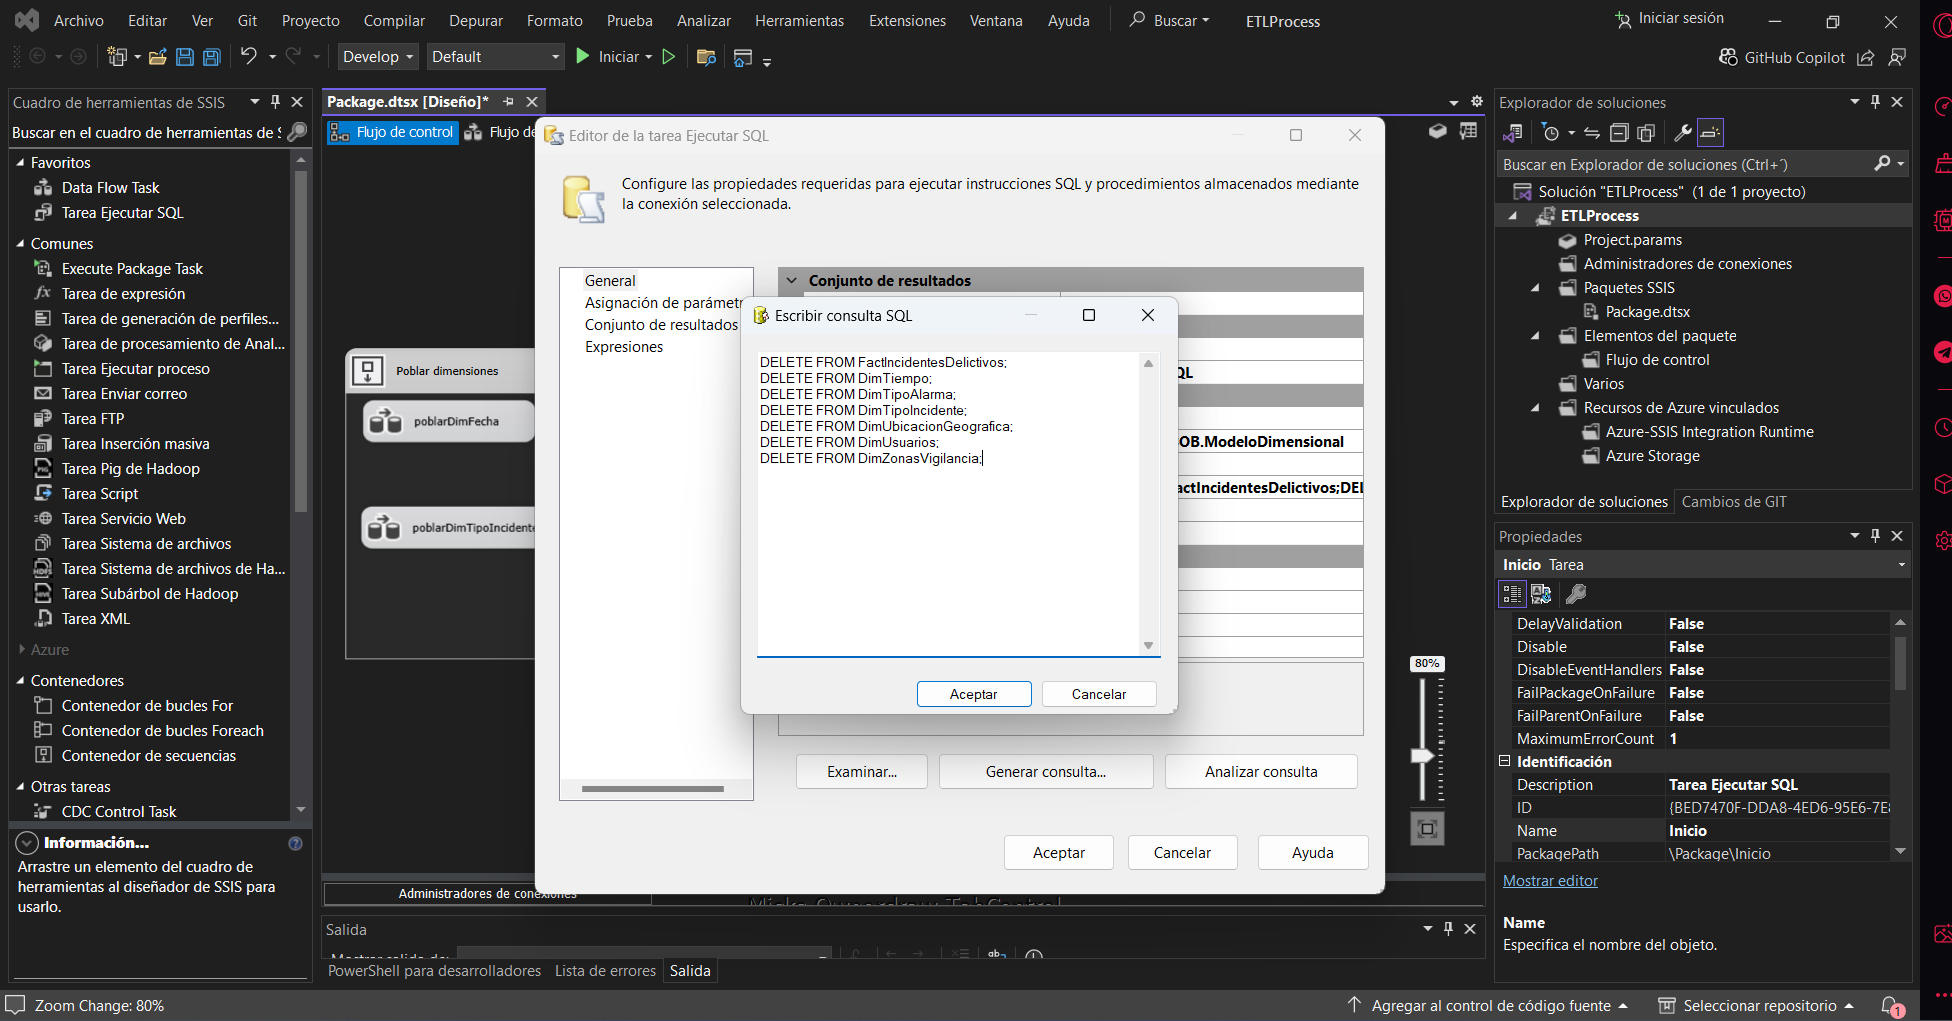
\includegraphics[width=0.8\textwidth]{chapters/III-resultados-y-discusion/resources/images/limpieza-bi.png}
    \caption{Limpieza de las tablas del modelo dimensional.}
    \label{fig:limpieza-bi}
\end{figure}

\begin{figure}[H]
    \centering
    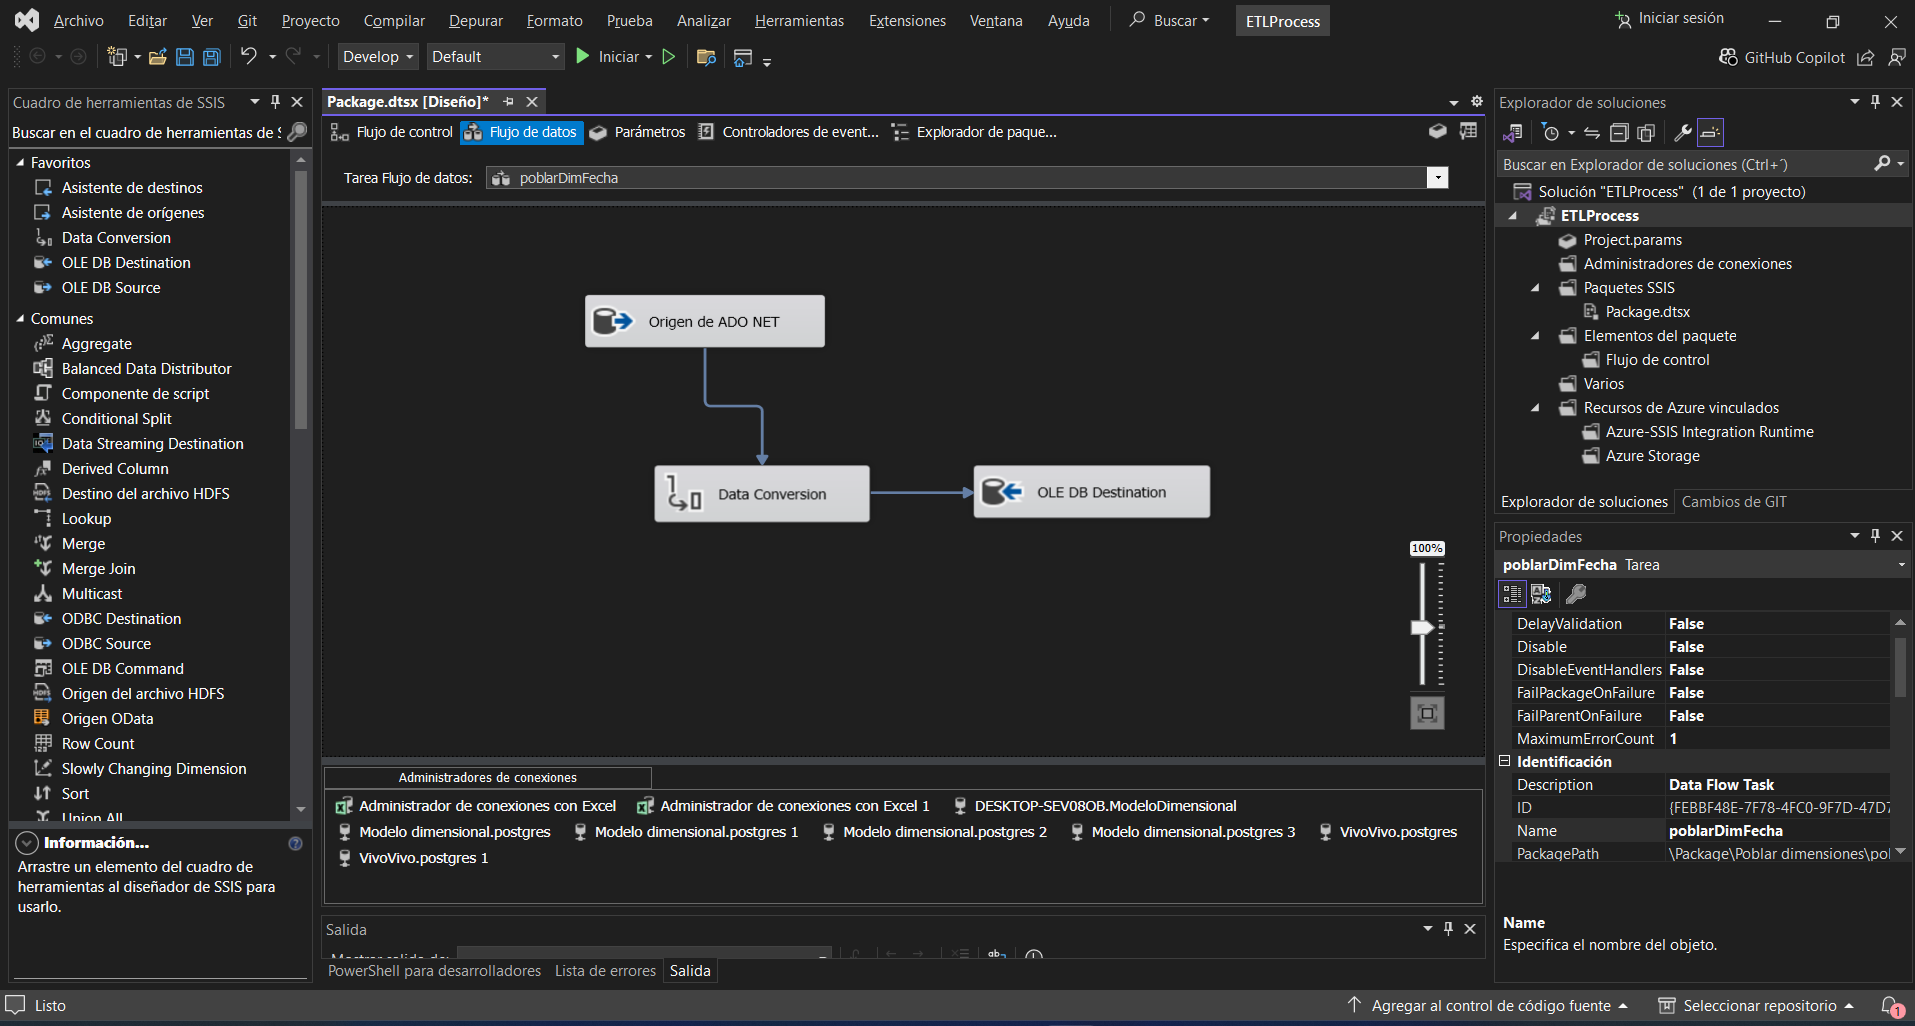
\includegraphics[width=0.8\textwidth]{chapters/III-resultados-y-discusion/resources/images/extraccion-bi.png}
    \caption{Extracción de datos para el modelo dimensional.}
    \label{fig:extraccion-bi}
\end{figure}

Al ejecutar el proceso ETL, se comienza con la extracción siguiendo el flujo de datos definido en el proceso ETL. En caso de no
existir ningún error, el sistema mostrará un mensaje de éxito, como se puede observar en la Figura \ref{fig:exito-bi}.

\begin{figure}[H]
    \centering
    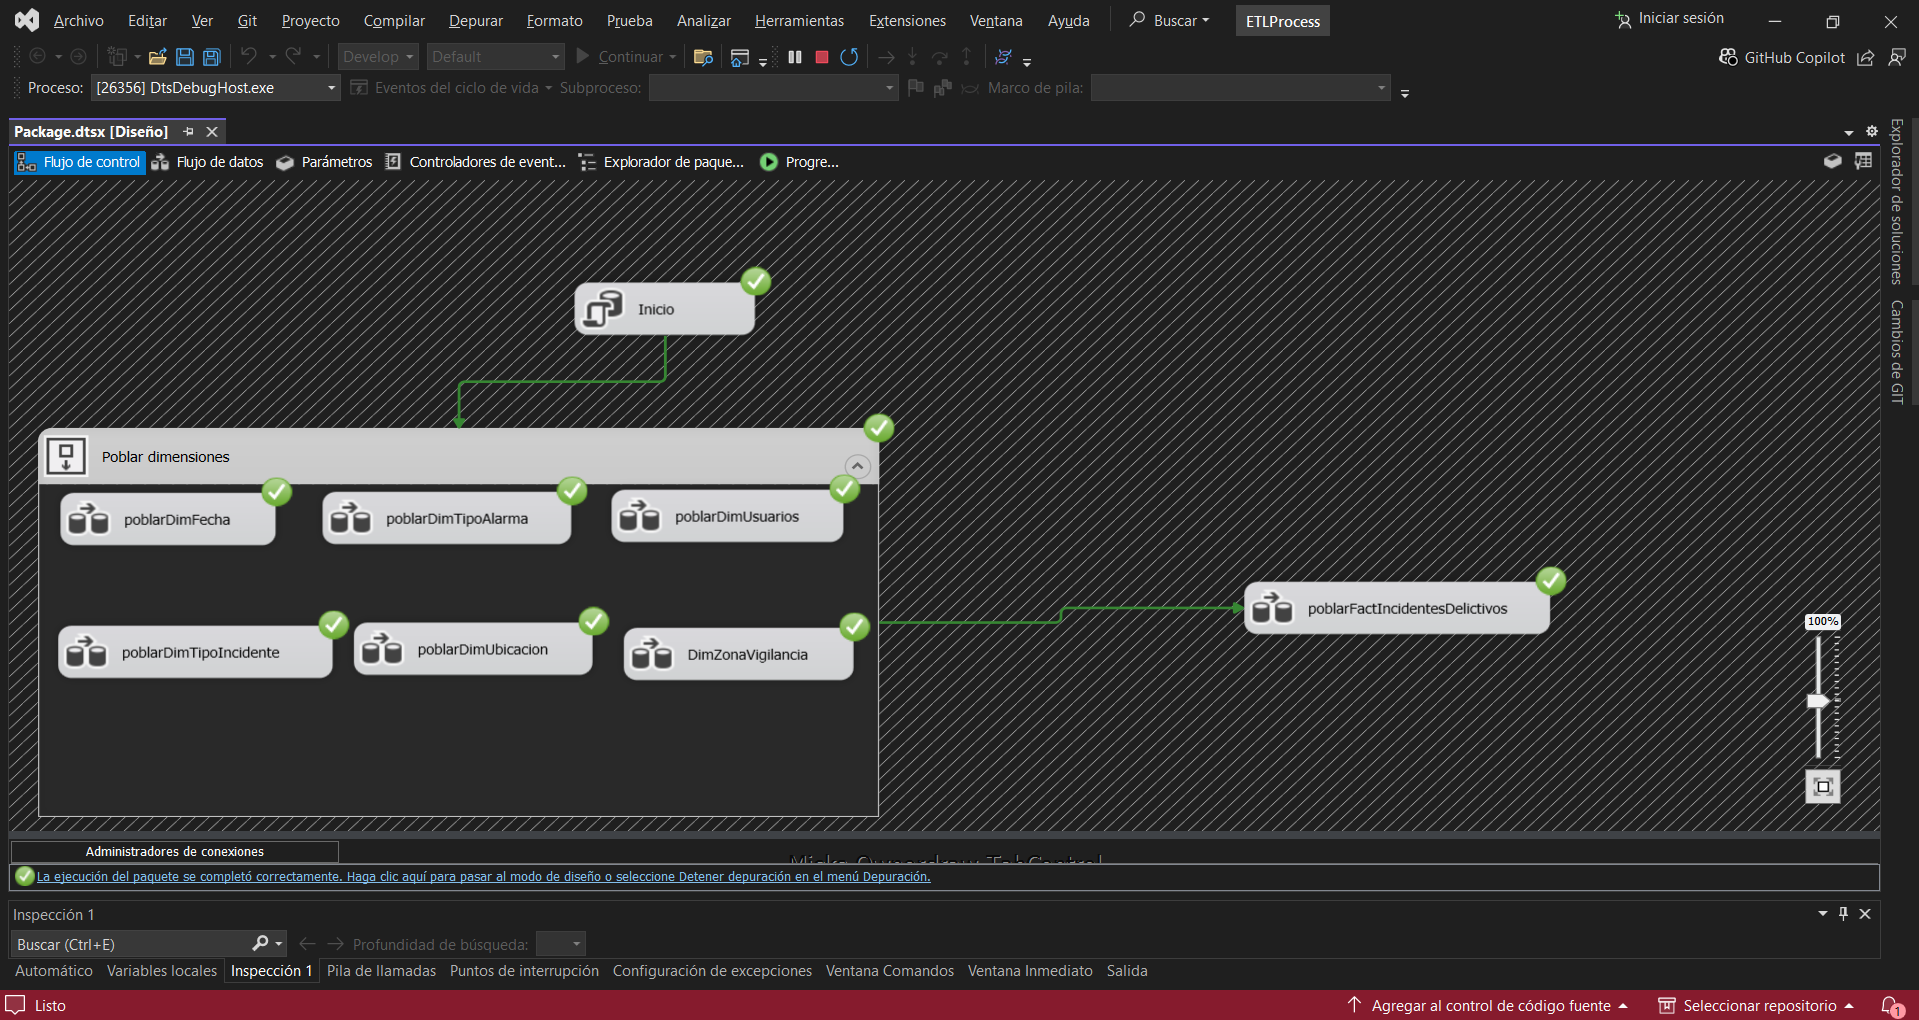
\includegraphics[width=0.8\textwidth]{chapters/III-resultados-y-discusion/resources/images/exito-bi.png}
    \caption{Mensaje de éxito al ejecutar el proceso ETL.}
    \label{fig:exito-bi}
\end{figure}

\paragraph{Cubo OLAP}
Para la construcción del cubo OLAP se empleó Visual Studio Community 2022, creando un proyecto de Analysis Services. En este
proyecto, se definió la conexión a la base de datos de SQL Server, como se muestra en la Figura \ref{fig:conexion-olap},
se creó un origen de datos, como se puede observar en la Figura \ref{fig:origen-datos-olap}, y se diseñó el cubo OLAP, como se
puede visualizar en la Figura \ref{fig:cubo-olap}.

\begin{figure}[H]
    \centering
    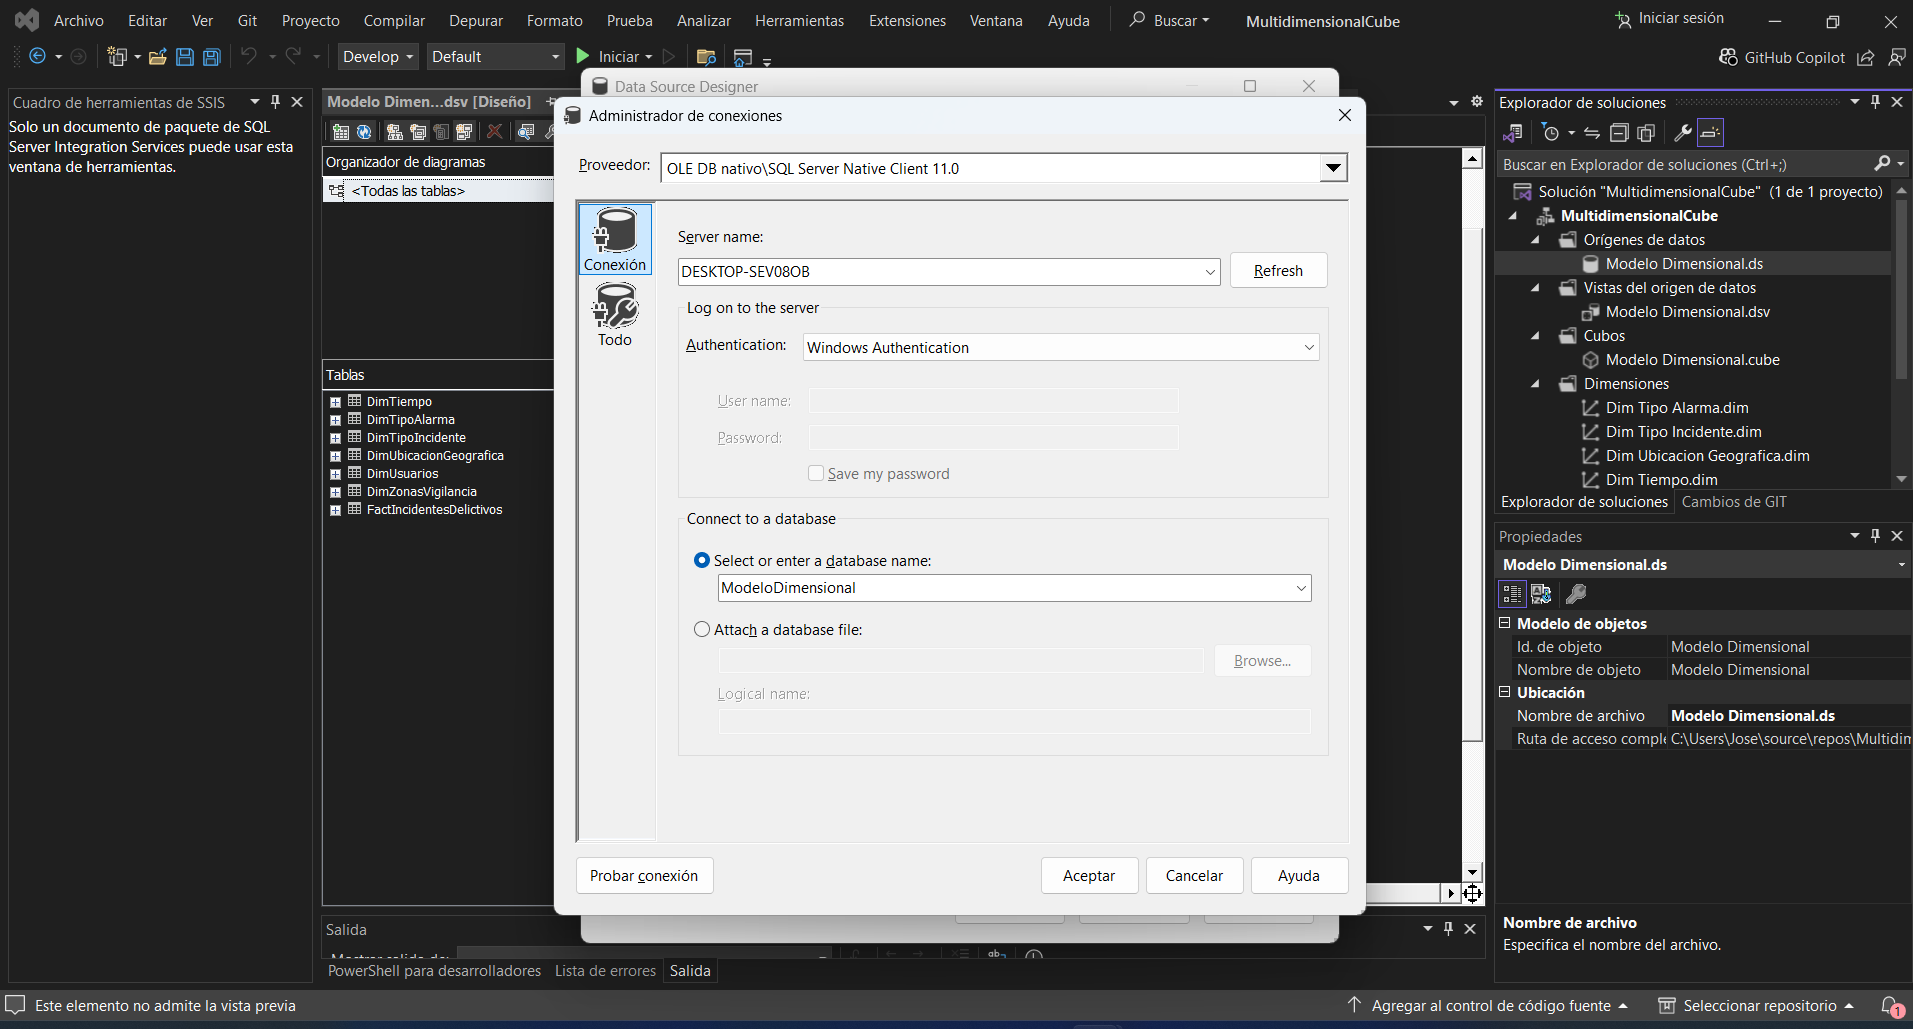
\includegraphics[width=0.8\textwidth]{chapters/III-resultados-y-discusion/resources/images/conexion-olap.png}
    \caption{Conexión a la base de datos de SQL Server en el proyecto de Analysis Services.}
    \label{fig:conexion-olap}
\end{figure}

\begin{figure}[H]
    \centering
    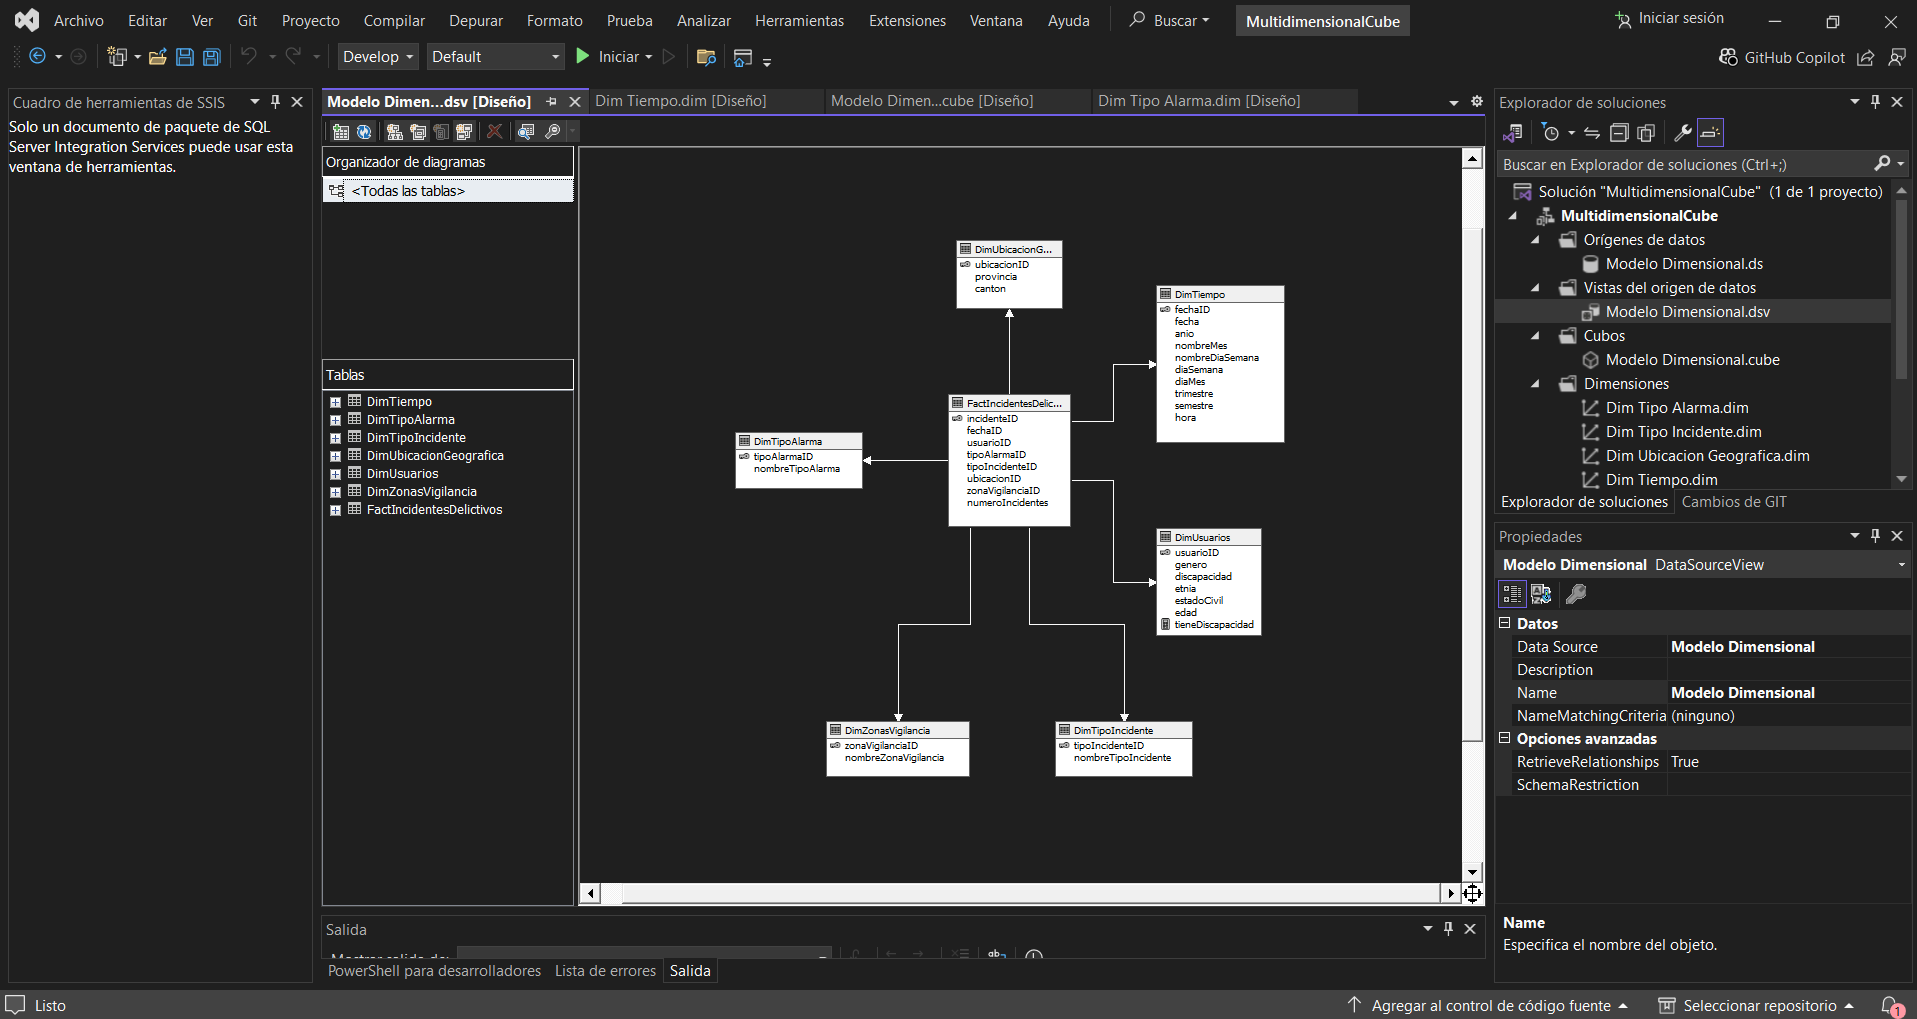
\includegraphics[width=0.8\textwidth]{chapters/III-resultados-y-discusion/resources/images/origen-datos-olap.png}
    \caption{Origen de datos en el proyecto de Analysis Services.}
    \label{fig:origen-datos-olap}
\end{figure}

\begin{figure}[H]
    \centering
    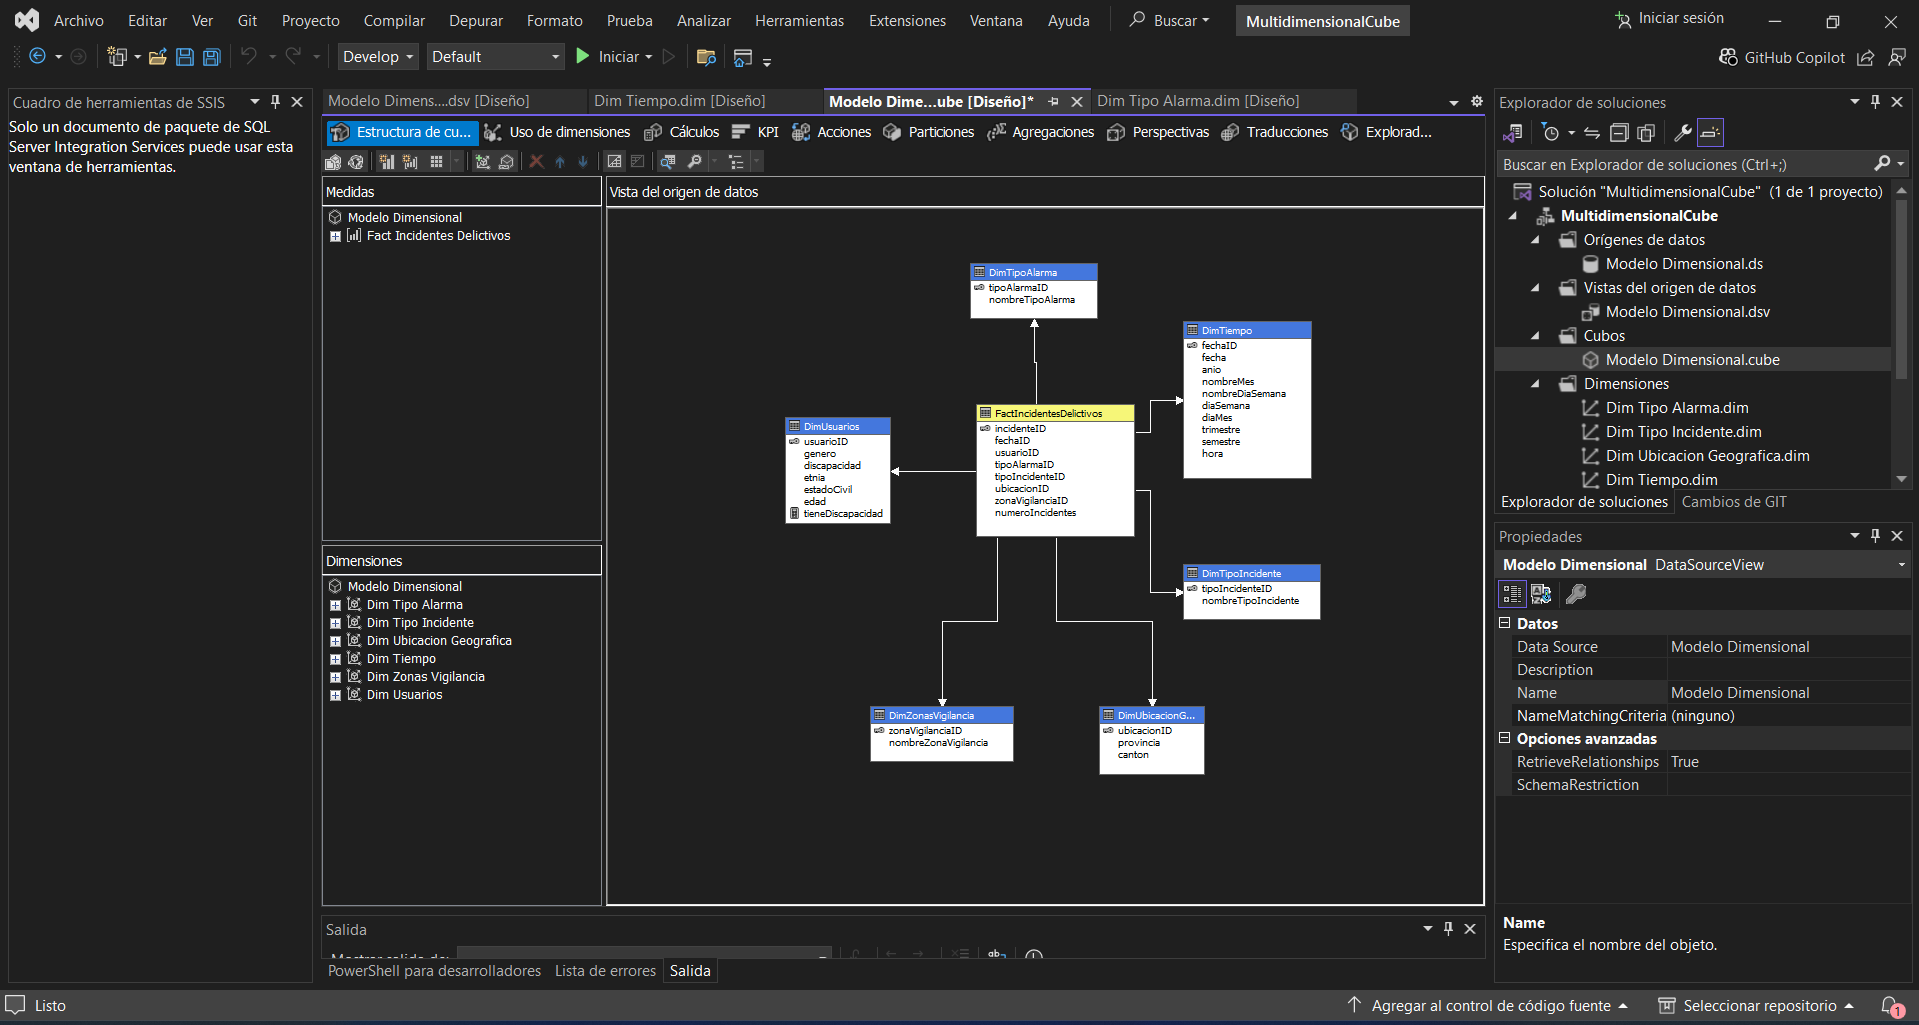
\includegraphics[width=0.8\textwidth]{chapters/III-resultados-y-discusion/resources/images/cubo-olap.png}
    \caption{Diseño del cubo OLAP en el proyecto de Analysis Services.}
    \label{fig:cubo-olap}
\end{figure}

En el origen de datos se definieron campos creados mediante cálculos con nombre que permiten agregar medidas e información
adicional al cubo OLAP, como se puede observar en la Figura \ref{fig:campos-origen-datos-olap}.

\begin{figure}[H]
    \centering
    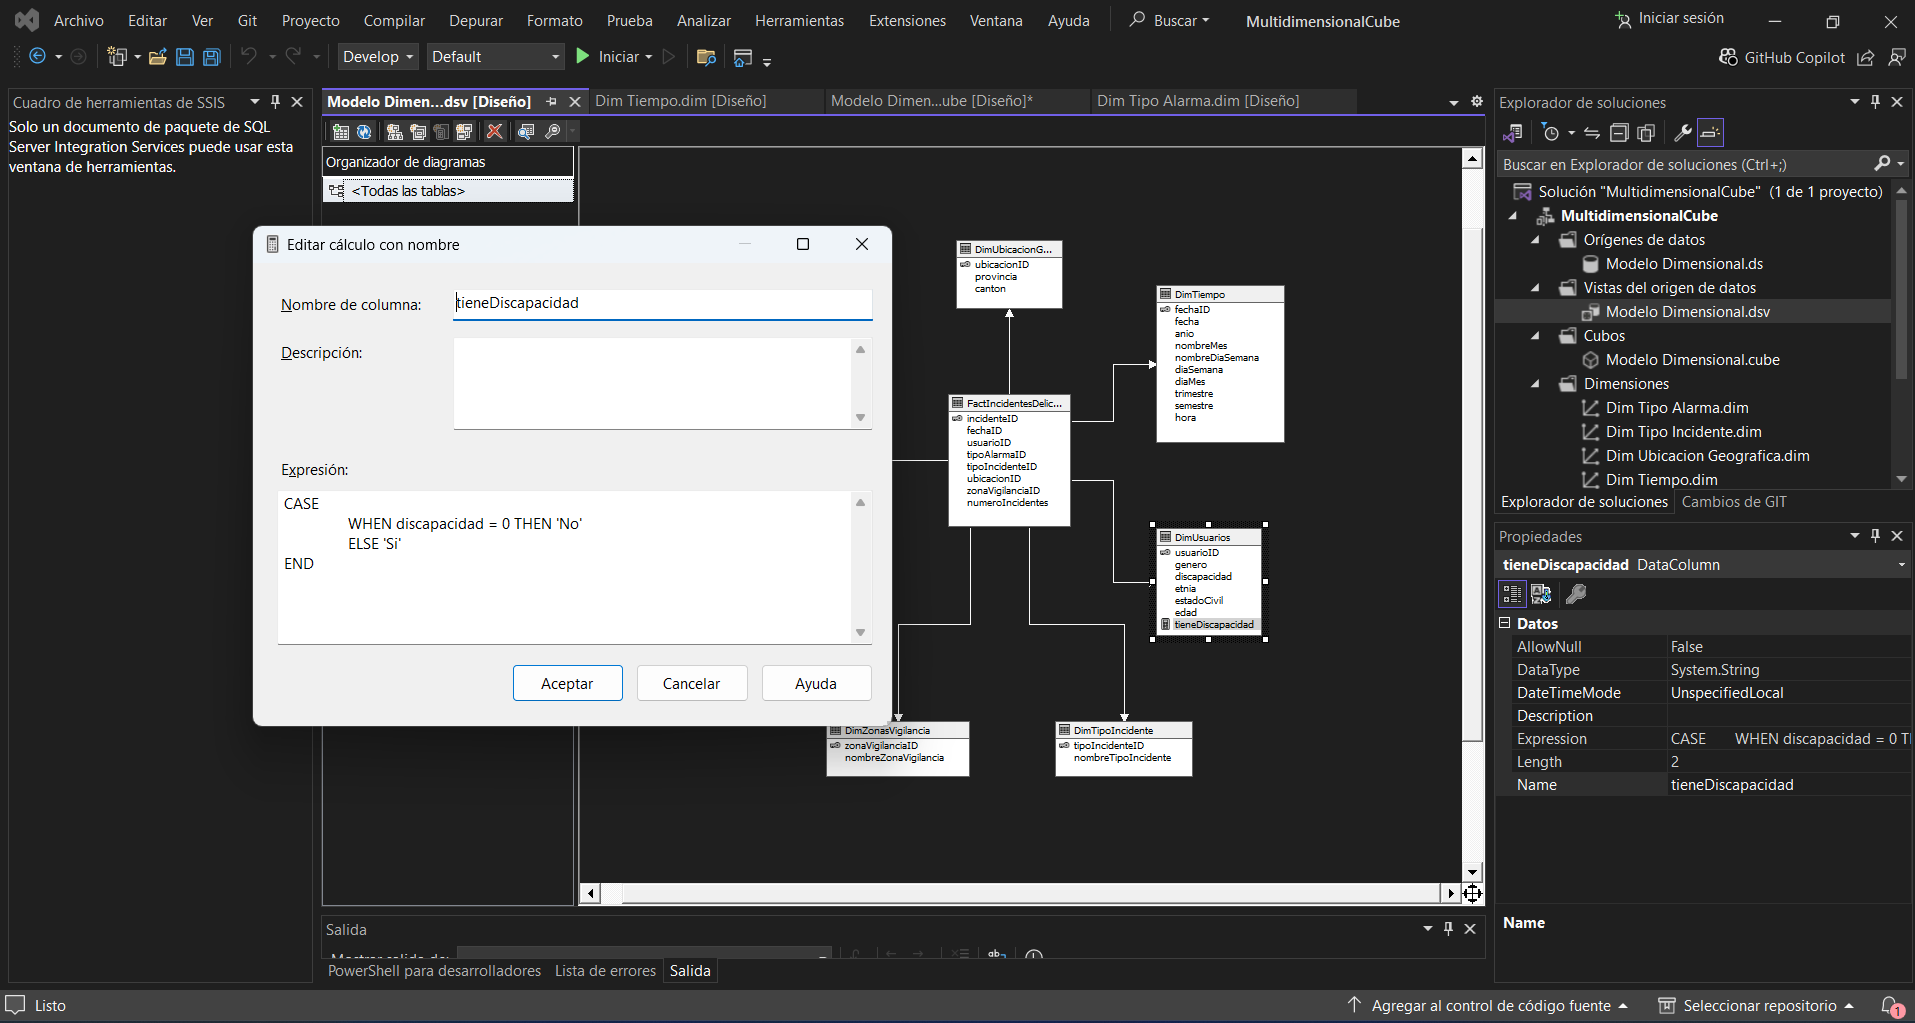
\includegraphics[width=0.8\textwidth]{chapters/III-resultados-y-discusion/resources/images/campos-origen-datos-olap.png}
    \caption{Campos en el origen de datos del proyecto de Analysis Services.}
    \label{fig:campos-origen-datos-olap}
\end{figure}

En la dimensión de tiempo se definieron jerarquías de tiempo que permiten visualizar los datos de forma secuencial en años, meses,
días y horas, como se puede observar en la Figura \ref{fig:dimension-tiempo-olap}.

\begin{figure}[H]
    \centering
    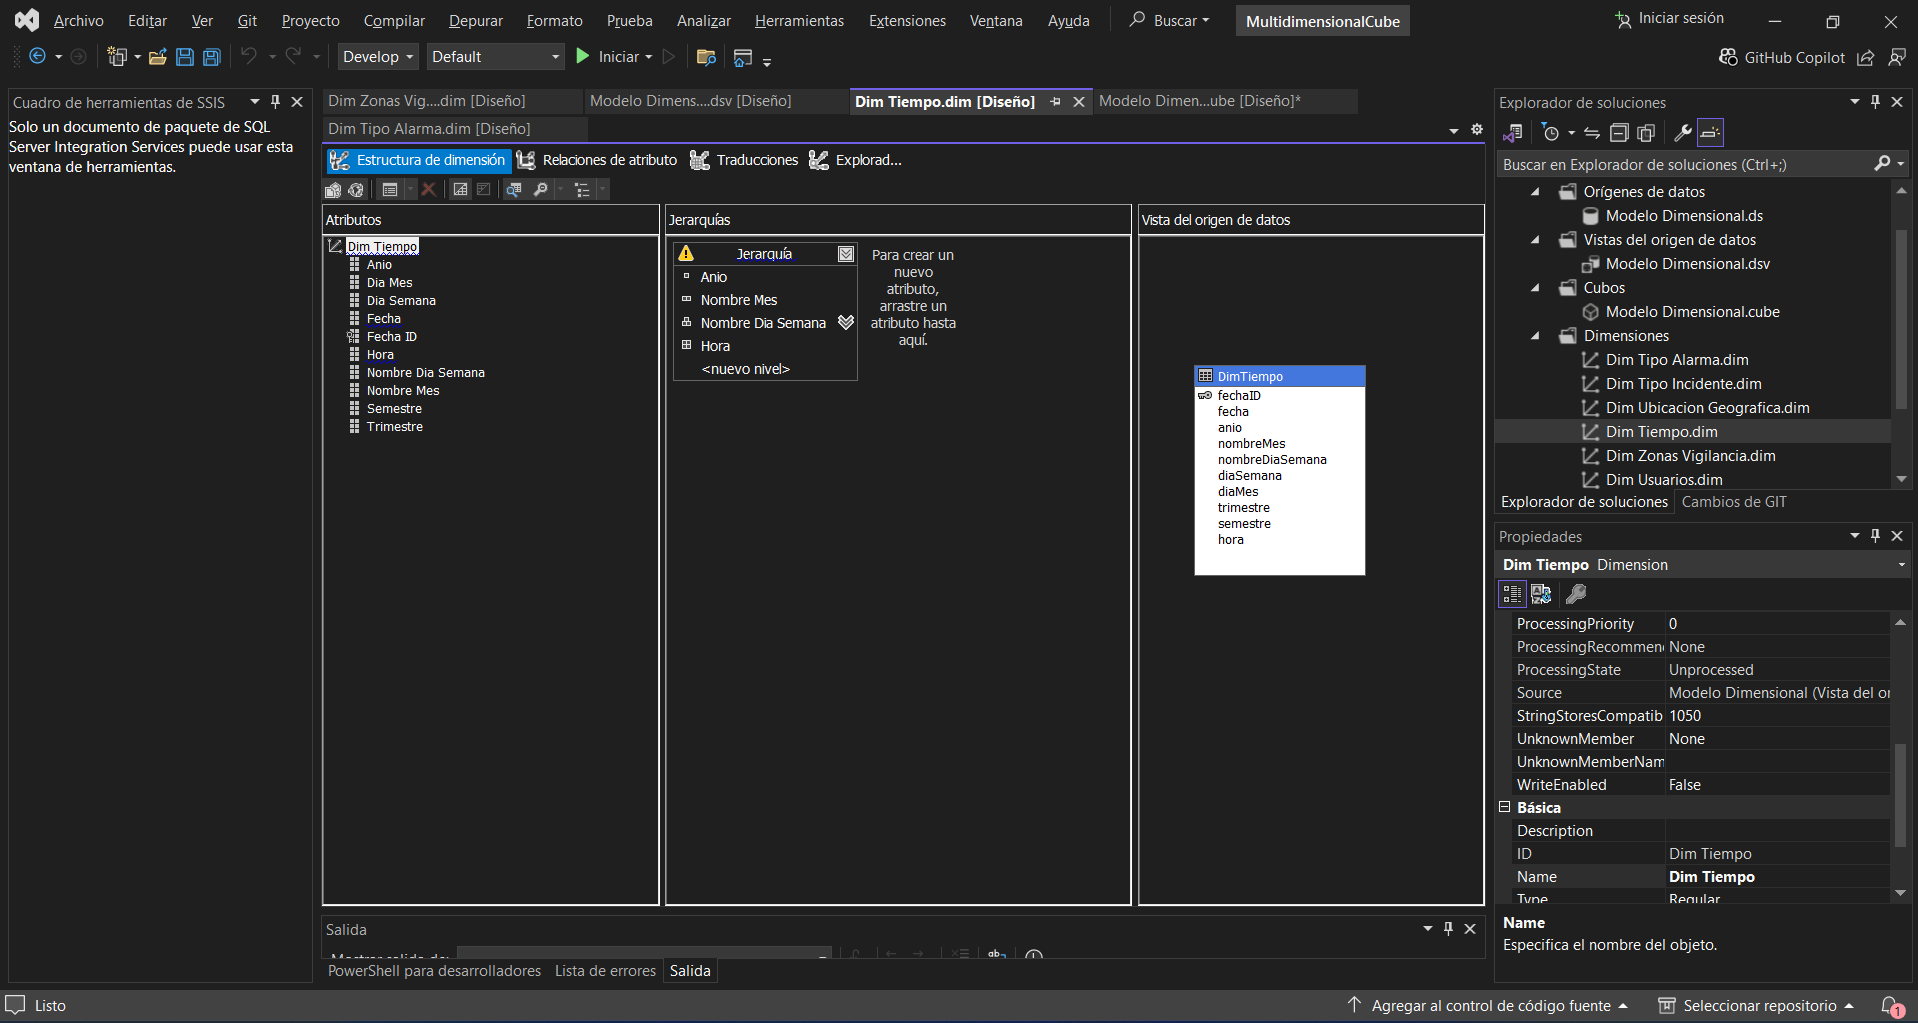
\includegraphics[width=0.8\textwidth]{chapters/III-resultados-y-discusion/resources/images/dimension-tiempo-olap.png}
    \caption{Jerarquías de tiempo en la dimensión de tiempo del proyecto de Analysis Services.}
    \label{fig:dimension-tiempo-olap}
\end{figure}

Una vez definido el cubo OLAP, se procedió a procesarlo para generar las medidas e indicadores definidos en el modelo dimensional, terminado
el proceso de procesamiento se muestra un mensaje de éxito y se muestra el examinador de cubos en el cual se pueden realizar consultas a los
datos del cubo OLAP, como se puede observar en la Figura \ref{fig:exito-olap}.

\begin{figure}[H]
    \centering
    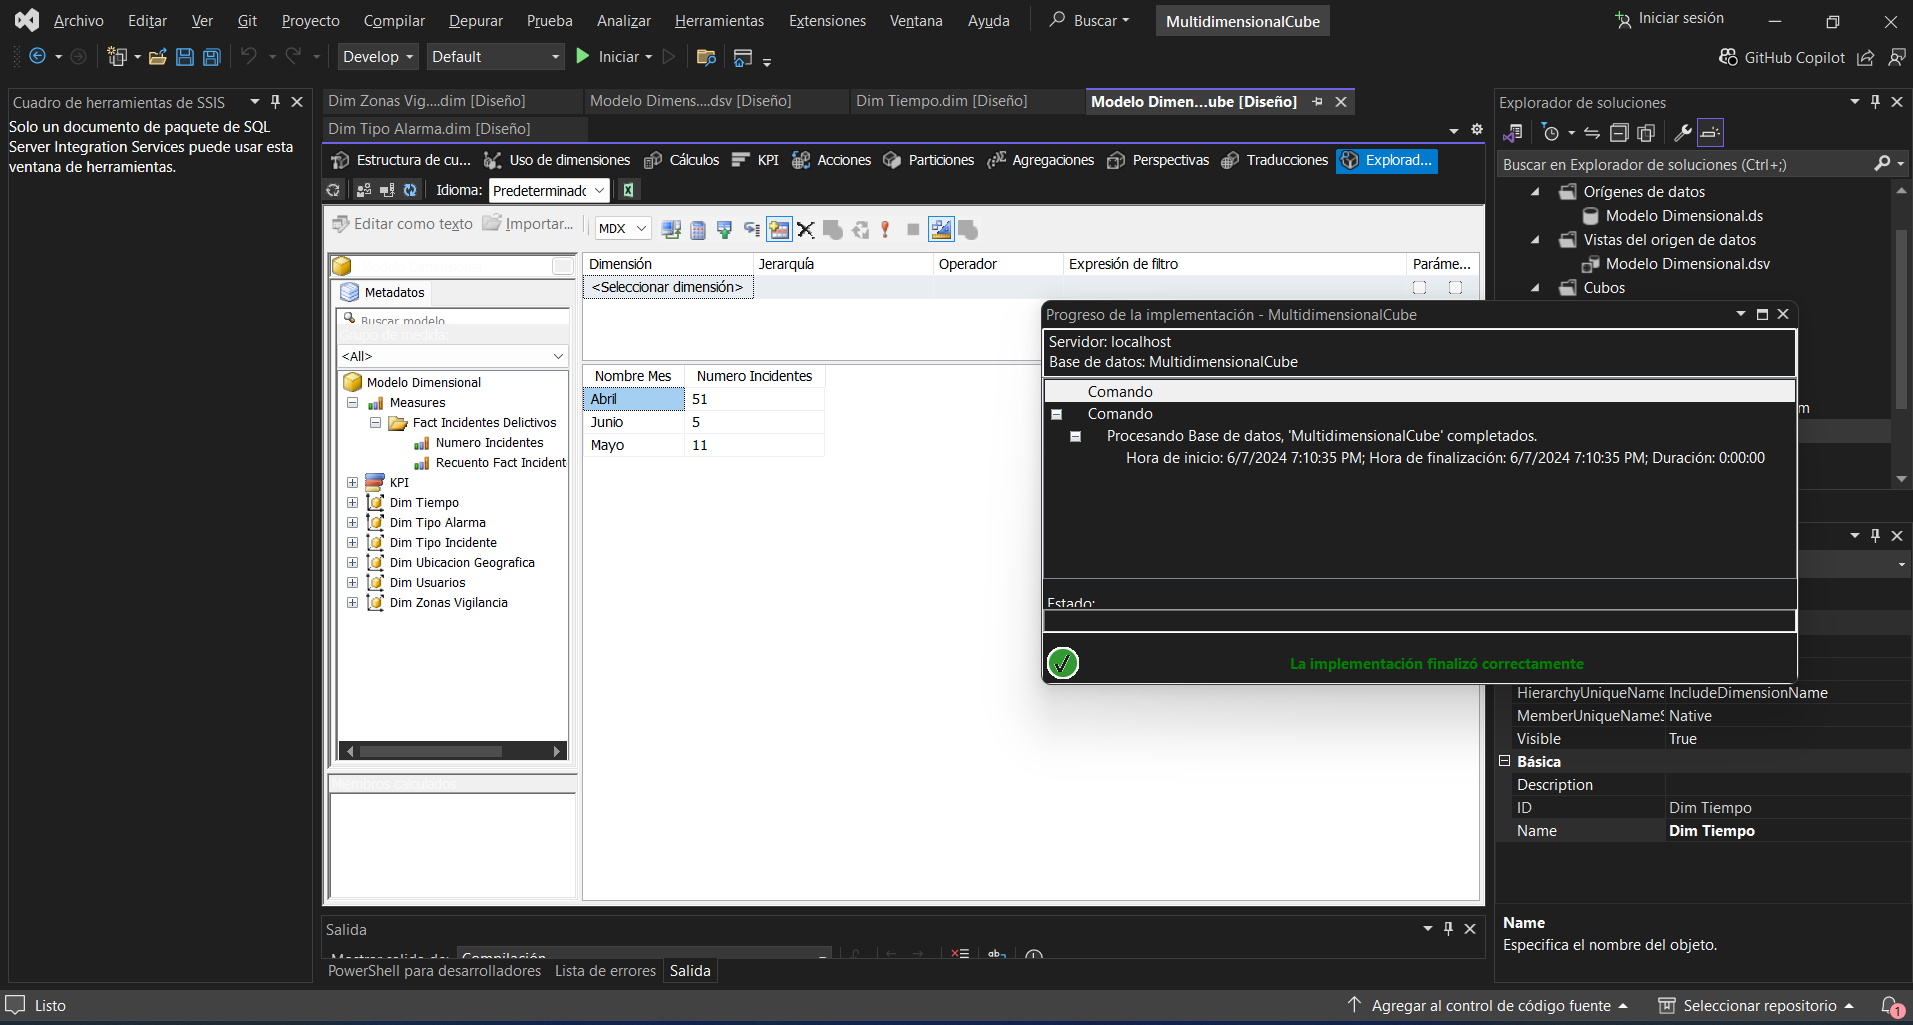
\includegraphics[width=0.8\textwidth]{chapters/III-resultados-y-discusion/resources/images/exito-olap.png}
    \caption{Mensaje de éxito al procesar el cubo OLAP.}
    \label{fig:exito-olap}
\end{figure}

\paragraph{Visualización de datos}
Para la visualización de datos se utilizó Power BI, el cual permite conectar a diferentes fuentes de datos, como SQL Server, Analysis Services,
Excel, entre otros. En este caso se lo conecto al cubo OLAP de Analysis Services, como se muestra en la Figura \ref{fig:conexion-bi}. Una vez
realizada la conexión En Power BI se creó un informe en el cual se visualizan los datos del cubo  mediante gráficos, tablas y mapas de calor
que permiten al usuario analizar la información de forma interactiva, como se muestra en la Figura \ref{fig:informe-bi}.

\begin{figure}[H]
    \centering
    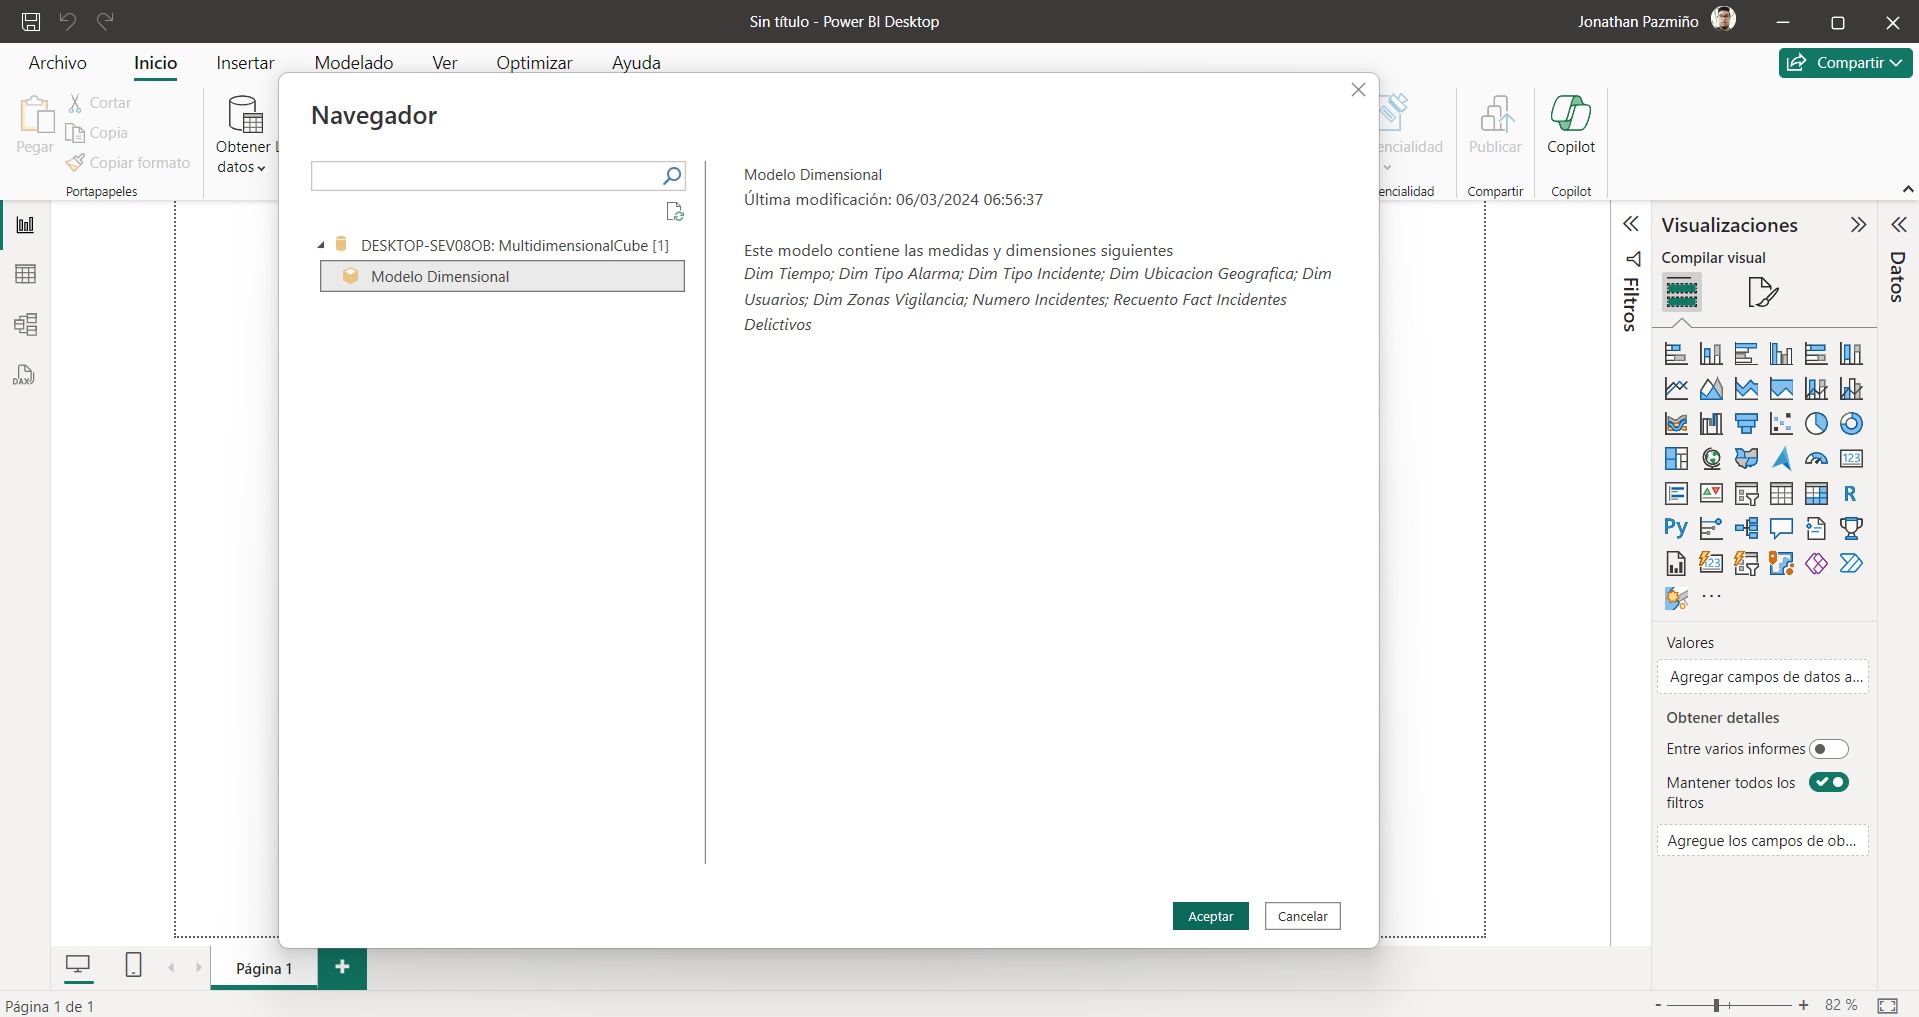
\includegraphics[width=0.8\textwidth]{chapters/III-resultados-y-discusion/resources/images/conexion-bi.png}
    \caption{Conexión al cubo OLAP de Analysis Services en Power BI.}
    \label{fig:conexion-bi}
\end{figure}

\begin{figure}[H]
    \centering
    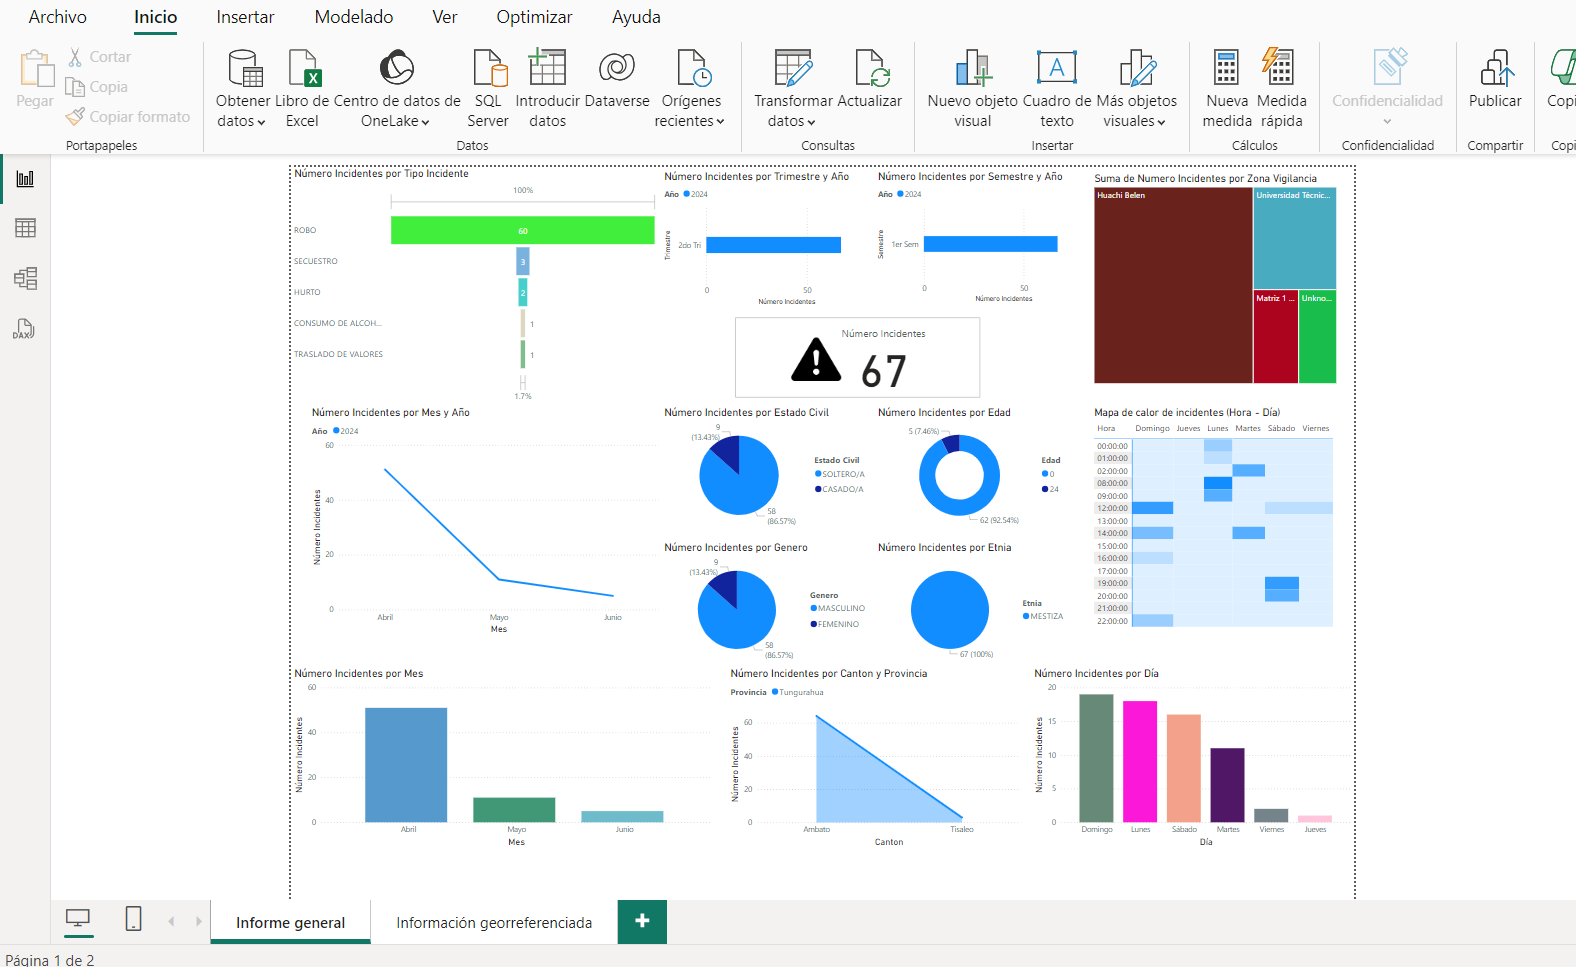
\includegraphics[width=0.8\textwidth]{chapters/III-resultados-y-discusion/resources/images/informe-bi.png}
    \caption{Informe en Power BI con los datos del cubo OLAP.}
    \label{fig:informe-bi}
\end{figure}

El informe en Power BI cuenta con filtros interactivos que permiten al usuario filtrar los datos por tiempo (Año, Mes, Día, Hora), tipo de
incidente, genero, etnia, estado civil, zona de vigilancia y edad de la víctima, como se puede observar en la Figura \ref{fig:filtros-bi}.

\begin{figure}[H]
    \centering
    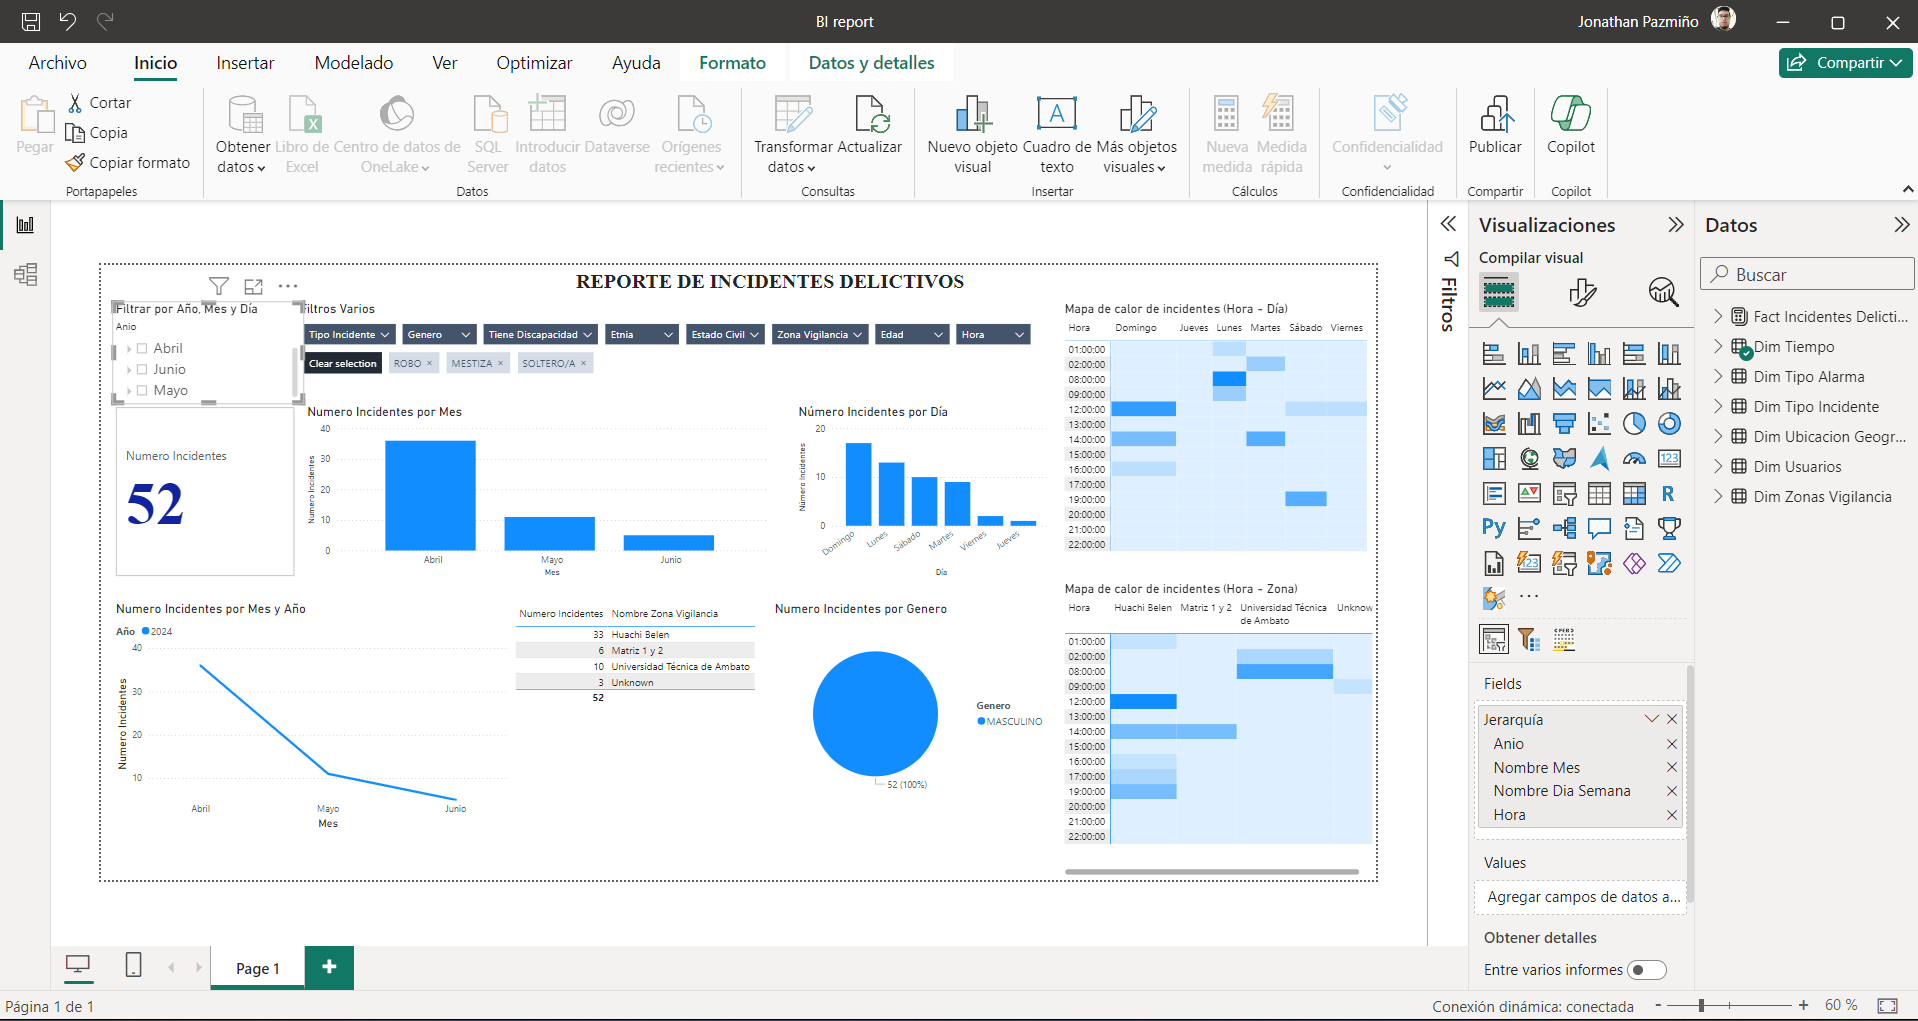
\includegraphics[width=0.8\textwidth]{chapters/III-resultados-y-discusion/resources/images/filtros-bi.png}
    \caption{Filtros interactivos en el informe de Power BI.}
    \label{fig:filtros-bi}
\end{figure}
